\chapter{Pump linearization and PI controller}
\label{cha:linear_pump}

The control structure chosen in \chapref{control_problem} and \figref{fig:control_structure} includes a PI controller, which is to designed. The PI controllers purpose is to use the optimized control output from the MPC as a control reference. 

The control focus of this project has been on the model predictive control, see \secref{sec:MPC}. Therefore a simple PI controller has been design, where the control structure can be seen on \figref{fig:simple_PI}.

\begin{figure}[H]
\centering
\begin{tikzpicture} [scale=0.8,transform shape]

\draw  (2.5,1) rectangle (4.5,0);
\node at (3.5,0.5) {G(s)};

\draw  (-1,1) rectangle (1,0);
\node at (0,0.5) {D(s)};

\draw[-triangle 60] (-3,0.5) -- (-1,0.5);
\draw[-triangle 60] (4.5,0.5) -- (6,0.5);
\draw[-triangle 60] (1,0.5) -- (2.5,0.5);
\draw[-triangle 60] (-5,0.5) -- (-3.5,0.5);
%\draw[-triangle 60] (-5.5,0.5) -- (-4.5,0.5);

\draw[-triangle 60] (5.25,0.5) -- (5.25,-1) -- (-3.25,-1) -- (-3.25,0.25);

%\node at (-5.5,1) {$CP_{ref}$};
\node at (-5,0.75) {$\Delta P_{ref}$};
\node at (-2.1,0.75) {$\Delta P_{error}$};
\node at (-3.75,0.8) {\large{$+$}};
\node at (-3.6,-0.08) {\large{$-$}};
\node at (5.25,0.75) {$\Delta p$};
\node at (1.75,0.75) {\large{$\omega$}};

\draw  (-3.25,0.5) ellipse (0.25 and 0.25);
\end{tikzpicture}%
  
\caption{The structure of the PI controller.}
\label{fig:simple_PI}
\end{figure}

The output from the MPC is a differential pressure, which is to be controlled through the rotational speed of the pumps. The model for the pumps is explained in \secref{PumpModel} and defined as

\begin{equation*}
\Delta p = -a_{h2}{q_i}^2 + a_{h1} \omega_r q_i + a_{h0}{\omega_r}^2
\end{equation*}

which is a nonlinear model. By the assumption that the flow is constant, the expression can through a Taylor expansion be linearized, with respect to $\omega$, to a small signal model.


For simplification the pump model is separated into smaller chunks, see \eqref{eq:tay_1}, then Taylor approximated, see \eqref{eq:tay_2}, where $\omega = \hat{\omega}+\bar{\omega}$.

\begin{equation}
\begin{split}
f_1(\bar{\omega}) &= a_{h1}\bar{q}\bar{\omega} \\
f_2(\bar{\omega}) &= a_{h0}\bar{\omega}^2
\end{split}
\label{eq:tay_1}
\end{equation}


\begin{equation}
\begin{split}
f_{t1}(\omega) &= f_1(\bar{\omega}) + f_1'(\bar{\omega})\cdot(\omega - \hat{\omega}) \\
f_{t2}(\omega) &= f_2(\bar{\omega}) + f_2'(\bar{\omega})\cdot(\omega - \hat{\omega})
\end{split}
\label{eq:tay_2}
\end{equation}

From \eqref{eq:tay_1} an expression for the workspace of, $\bar{\Delta P}$, can be made.

\begin{equation}
\begin{split}
\bar{\Delta P} = f_{1}(\bar{\omega}) + f_{2}(\bar{\omega}) + c
\end{split}
\label{eq:tay_3}
\end{equation}

The linear pump model can then be expressed as seen in \eqref{eq:tay_4}

\begin{equation}
\begin{split}
0 &= -(\bar{\Delta P} + \hat{\Delta P}) + f_{t1}(\bar{\omega}) + f_{t2}(\bar{\omega}) + c\\
  &= -(f_{1}(\bar{\omega}) + f_{2}(\bar{\omega}) + c + \hat{\Delta P}) + f_{t1}(\bar{\omega}) + f_{t2}(\bar{\omega}) + c \\ 
  &= -\hat{\Delta P} + f_1'(\bar{\omega})\cdot\hat{\omega} + f_2'(\bar{\omega})\cdot\hat{\omega}
\end{split}
\label{eq:tay_4}
\end{equation}

\eqref{eq:tay_4} is then Laplace transformed and solved for the input output relationship as seen on \figref{fig:simple_PI}

\begin{equation}
G(s) = \frac{\Delta P}{\omega} = f'_1(\bar{\omega}) + f'_2(\bar{\omega}) = a_{h1}\bar{q} + 2a_{h0}\bar{\omega}
\label{eq:lin_pump_simon}
\end{equation}

With the following operating points set for the pumps, the differential pressure over the pumps and their respective valves are measured. 

\begin{equation}
\centering
	\begin{split}
	\omega_{C18} &= 0.16,\hspace{20pt} \Delta P_{C18} = 0.0807 \\
	\omega_{C25} &= 0.4,\hspace{20pt} \Delta P_{C25} = 0.255  \\
	\omega_{C2}  &= 0.4,\hspace{20pt} \Delta P_{C2} = 0.2 \\
	\omega_{C16} &= 0.4,\hspace{20pt} \Delta P_{C16} =0.25 
	\end{split}
\end{equation}

From this the flow through the pumps can be estimated through \eqref{omega_notzero}, with their respective pump parameters found in \appref{system_description}.

\begin{equation}
\centering
\begin{split}
q_{C18} &= 0.179 \hspace{20pt} q_{C25} &= 0.272 \hspace{20pt} q_{C2} &= 0.061 \hspace{20pt} q_{C16} &= 0.169
\end{split}
\end{equation}

By inserting the values for the linearized model in \eqref{eq:lin_pump_simon}, the final models ends up as gains. 

\begin{equation}
\centering
	\begin{split}
	G_{C18}(s) &= 0.218 \hspace{20pt} G_{C25}(s) &= 0.548 \hspace{20pt} G_{C2}(s) &= 0.962 \hspace{20pt} G_{C16}(s) &= 0.963
	\end{split}
\end{equation}

As it can be seen in \todo{add secref} is the dynamic of the system slow. Therefore will a controller that can react within 3-5 seconds be fast enough.
By using the Matlab design tool box for dynamical systems and having the settling time of 3 seconds in mind, the gains for the PI controller can be found as shown in \eqref{eq:PI_GAINS}. 
Due to high similarities between these controllers only one step response in shown on \figref{fig:Tikz_PI_PUMP_GAIN}.

\begin{equation}
\centering
	\begin{split}
	K_{C18} &= 8 \hspace{20pt} K_{C25} &= 3 \hspace{20pt} K_{C2} &= 2 \hspace{20pt} K_{C16} &= 2
	\end{split}
	\label{eq:PI_GAINS}
\end{equation}

\begin{figure}[H]
\centering
% This file was created by matlab2tikz.
%
%The latest updates can be retrieved from
%  http://www.mathworks.com/matlabcentral/fileexchange/22022-matlab2tikz-matlab2tikz
%where you can also make suggestions and rate matlab2tikz.
%
\definecolor{mycolor1}{rgb}{0.00000,0.44700,0.74100}%
%
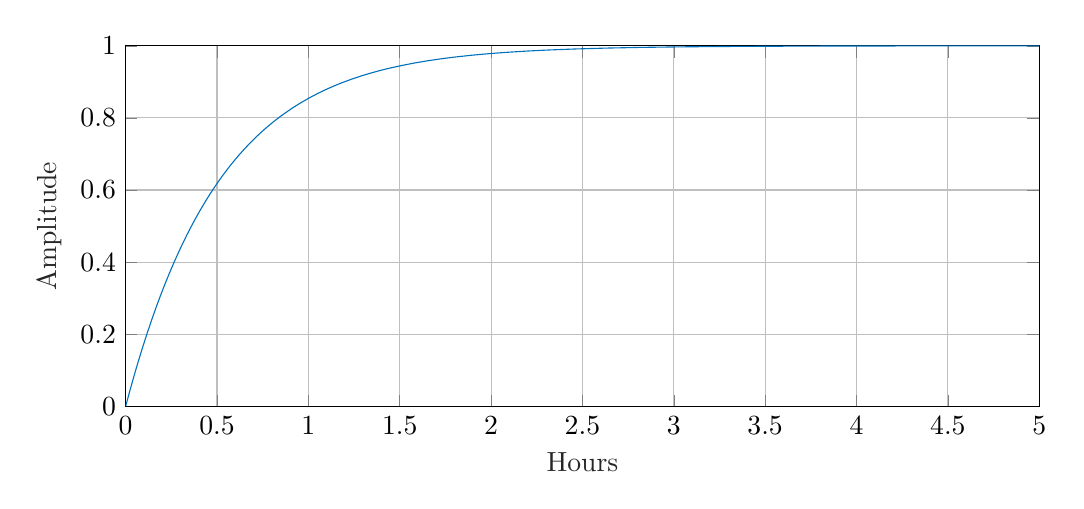
\begin{tikzpicture}

\begin{axis}[%
width=4.568in,
height=1.803in,
at={(0.766in,0.486in)},
scale only axis,
xmin=0,
xmax=5,
xlabel style={font=\color{white!15!black}},
xlabel={Hours},
ymin=0,
ymax=1,
ylabel style={font=\color{white!15!black}},
ylabel={Amplitude},
axis background/.style={fill=white},
xmajorgrids,
ymajorgrids
]

\addplot [color=mycolor1, forget plot]
  table[row sep=crcr]{%
0	0\\
0.0239225439509072	0.045007413978559\\
0.0478450879018153	0.0879891606440806\\
0.0717676318527225	0.129036410043906\\
0.0956901758036306	0.168236228897311\\
0.119612719754538	0.205671765275698\\
0.143535263705446	0.241422424970792\\
0.167457807656353	0.275564039924983\\
0.19138035160726	0.308169029081034\\
0.215302895558168	0.339306551992372\\
0.239225439509076	0.369042655519773\\
0.263147983459984	0.397440413925607\\
0.287070527410891	0.424560062662806\\
0.310993071361799	0.450459126142338\\
0.334915615312706	0.475192539750188\\
0.358838159263613	0.498812766372688\\
0.382760703214521	0.521369907677321\\
0.406683247165429	0.542911810385084\\
0.430605791116337	0.563484167759793\\
0.454528335067244	0.583130616529623\\
0.478450879018152	0.60189282944646\\
0.502373422969059	0.619810603679396\\
0.526295966919966	0.636921945229856\\
0.550218510870875	0.653263149547426\\
0.574141054821782	0.668868878517366\\
0.59806359877269	0.68377223398312\\
0.621986142723597	0.698004827959757\\
0.645908686674505	0.711596849687298\\
0.669831230625412	0.724577129666142\\
0.69375377457632	0.736973200810422\\
0.717676318527228	0.748811356849002\\
0.741598862478135	0.760116708098011\\
0.765521406429043	0.770913234723183\\
0.78944395037995	0.781223837605006\\
0.813366494330858	0.791070386914558\\
0.837289038281765	0.800473768503075\\
0.861211582232673	0.809453928203639\\
0.909056670134488	0.826219917125028\\
0.956901758036303	0.841510680753855\\
1.00474684593812	0.855456022925375\\
1.05259193383993	0.868174326144328\\
1.10043702174175	0.879773556538229\\
1.14828210964356	0.890352180385653\\
1.19612719754538	0.899999999999974\\
1.24397228544719	0.908798916064383\\
1.29181737334901	0.916823622889709\\
1.33966246125082	0.924142242497059\\
1.38750754915264	0.930816902908085\\
1.43535263705446	0.93690426555196\\
1.50712026890718	0.945045912614219\\
1.5788879007599	0.952136990767719\\
1.65065553261262	0.958313061652951\\
1.72242316446535	0.963692194522975\\
1.79419079631807	0.968377223398304\\
1.8898809721217	0.973697320081035\\
1.98557114792533	0.978122383760494\\
2.08126132372896	0.981802991413891\\
2.2008740434835	0.985545602292533\\
2.32048676323804	0.988518463785025\\
2.46402202694348	0.991290364100434\\
2.63147983459983	0.993690426555194\\
2.82286018620709	0.995634841677595\\
3.06208562571617	0.99724577129666\\
3.37307869707797	0.998486438751562\\
3.80368448819431	0.999339306551992\\
4.49743826277063	0.999826219917124\\
5.02373422969059	0.999936904265551\\
};
\end{axis}


\end{tikzpicture}%
\caption{Step response of one pump PI system.}
\label{fig:Tikz_PI_PUMP_GAIN}
\end{figure}

\subsection*{PI test}

The PI controller was implemented on the water system described in \chapref{system_overview}. From the test it where concluded that some tuning of the gains had to be done, due to large overshoots and marginal stabilities on some of the pumps. The final values where found by trail and errors and can be seen in \eqref{eq:NEW_PI_GAINS}. 

\begin{equation}
\centering
	\begin{split}
	K_{C18} &= 6 \hspace{20pt} K_{C25} &= 4 \hspace{20pt} K_{C2} &= 1.4 \hspace{20pt} K_{C16} &= 1.4
	\end{split}
	\label{eq:NEW_PI_GAINS}
\end{equation}

Whit these gains the systems gets a slower response than the settling time of 4 seconds. However this is still deemed fit to this project, since dynamics of the WT is much slower.

\begin{figure}[H]
\centering
% This file was created by matlab2tikz.
%
%The latest updates can be retrieved from
%  http://www.mathworks.com/matlabcentral/fileexchange/22022-matlab2tikz-matlab2tikz
%where you can also make suggestions and rate matlab2tikz.
%
\definecolor{mycolor1}{rgb}{0.00000,0.44700,0.74100}%
\definecolor{mycolor2}{rgb}{0.85000,0.32500,0.09800}%
\definecolor{mycolor3}{rgb}{0.92900,0.69400,0.12500}%
\definecolor{mycolor4}{rgb}{0.49400,0.18400,0.55600}%
%
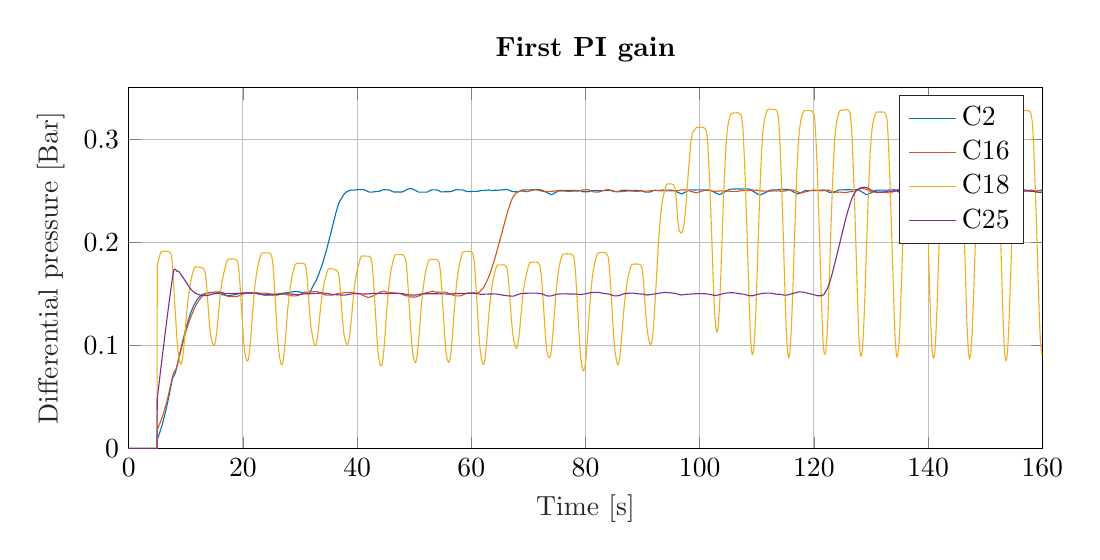
\begin{tikzpicture}

\begin{axis}[%
width=4.568in,
height=1.803in,
at={(0.766in,0.486in)},
scale only axis,
xmin=0,
xmax=160,
xlabel style={font=\color{white!15!black}},
xlabel={Time [s]},
ymin=0,
ymax=0.35,
ylabel style={font=\color{white!15!black}},
ylabel={Differential pressure [Bar]},
axis background/.style={fill=white},
title style={font=\bfseries},
title={First PI gain},
xmajorgrids,
ymajorgrids,
legend style={legend cell align=left, align=left, draw=white!15!black}
]
\addplot [color=mycolor1]
  table[row sep=crcr]{%
0	0\\
4.94999999999999	0\\
5	0.00897482893449819\\
5.15000000000001	0.0110153958944181\\
5.40000000000001	0.0148765884652846\\
5.75	0.020821114369511\\
5.84999999999999	0.0226539589442893\\
6.19999999999999	0.0300464320625622\\
6.34999999999999	0.0333760997067429\\
6.5	0.0368707233626537\\
6.84999999999999	0.0454667644183644\\
7.05000000000001	0.0507025904203431\\
7.34999999999999	0.0589870478983414\\
7.65000000000001	0.0673448191593309\\
7.69999999999999	0.0683223362658794\\
8.05000000000001	0.0719452590420246\\
8.09999999999999	0.0725256598240378\\
8.15000000000001	0.0733015640273607\\
8.30000000000001	0.0761608015640149\\
8.34999999999999	0.0772299608993023\\
8.55000000000001	0.0821664222874006\\
8.90000000000001	0.0908296676441864\\
9.09999999999999	0.0957783479960881\\
9.44999999999999	0.104062805474086\\
9.94999999999999	0.115090420332365\\
10.15	0.119189882697952\\
10.4	0.123863636363637\\
10.65	0.128299120234601\\
10.85	0.131561583577707\\
11.25	0.137035679374378\\
11.5	0.13977883675463\\
11.85	0.143310117302065\\
12.05	0.145002443792777\\
12.25	0.146383186705776\\
12.6	0.148350439882705\\
12.85	0.149309628543506\\
13.15	0.150000000000006\\
13.45	0.150433773216037\\
13.65	0.150592619745851\\
13.95	0.150922531769311\\
14.3	0.151105816226789\\
14.7	0.151093597262957\\
14.95	0.151050830889545\\
15.25	0.151075268817209\\
15.55	0.15078812316716\\
16	0.150018328445753\\
16.45	0.149260752688178\\
17.2	0.148234359726303\\
17.75	0.148466520039108\\
18.8	0.149627321603134\\
19.55	0.150439882697952\\
19.7	0.150708699902253\\
20.25	0.150769794721413\\
20.45	0.15098362658847\\
21.2	0.151246334310855\\
22.45	0.15081867057674\\
24.1	0.148930840664718\\
24.95	0.148936950146634\\
25.3	0.149028592375373\\
25.5	0.149120234604112\\
26	0.14979838709678\\
26.35	0.150152737047904\\
26.55	0.150250488758559\\
27	0.150794232649076\\
27.3	0.150891984359731\\
27.5	0.150995845552302\\
27.75	0.1511485826002\\
28.3	0.151600684261979\\
28.55	0.151906158357775\\
29.2	0.152492668621704\\
29.9	0.151930596285439\\
30.2	0.151594574780063\\
30.45	0.151325757575762\\
30.75	0.151032502443798\\
31.1	0.150598729227767\\
31.25	0.150769794721413\\
31.65	0.151771749755625\\
31.75	0.152315493646142\\
31.9	0.153274682306943\\
31.95	0.153757331378301\\
32.2	0.156860948191593\\
32.8	0.16270161290322\\
32.95	0.164595552297158\\
33.1	0.166544477028339\\
33.65	0.174816715542534\\
33.75	0.176282991202356\\
34.15	0.183241691104598\\
34.65	0.192906891495596\\
34.95	0.199340175953068\\
35.5	0.2113086510264\\
35.65	0.214589442815253\\
36.15	0.225800342130981\\
36.25	0.227920332355808\\
36.55	0.233748778103632\\
36.7	0.236430840664724\\
36.9	0.239473362658856\\
36.95	0.24002321603129\\
37.2	0.24206378299121\\
37.6	0.245839442815253\\
37.75	0.246981915933532\\
37.85	0.247635630498536\\
38.1	0.24881476050831\\
38.4	0.249761730205279\\
38.85	0.2506903714565\\
39	0.250843108504398\\
39.5	0.250727028347995\\
39.85	0.251160801564026\\
40.2	0.251295210166177\\
41.2	0.251179130009774\\
41.4	0.250739247311827\\
41.75	0.249847262952102\\
41.95	0.249181329423266\\
42.2	0.248771994134898\\
42.65	0.248881964809385\\
43.75	0.249566226783969\\
44	0.249761730205279\\
44.6	0.251228005865102\\
44.75	0.251228005865102\\
45.65	0.250800342130987\\
45.8	0.250574291300097\\
46.1	0.249566226783969\\
46.35	0.249040811339199\\
46.6	0.248894183773217\\
47.9	0.24897971652004\\
48.2	0.249731182795699\\
48.85	0.251588465298141\\
49.05	0.251997800586508\\
49.6	0.252138318670575\\
49.7	0.251967253176929\\
50.05	0.250946969696969\\
50.25	0.250378787878788\\
50.45	0.249792277614858\\
50.7	0.249046920821115\\
50.8	0.248826979472142\\
51.15	0.248826979472142\\
51.35	0.248808651026394\\
51.9	0.248820869990226\\
52.25	0.248863636363637\\
52.35	0.249046920821115\\
52.8	0.250610948191593\\
52.9	0.250800342130987\\
53.2	0.251008064516128\\
53.65	0.25102028347996\\
53.9	0.250928641251221\\
54.2	0.250549853372434\\
54.45	0.249773949169111\\
54.65	0.249138563049854\\
54.95	0.249004154447704\\
55.25	0.249132453567938\\
55.4	0.249126344086022\\
55.9	0.249248533724341\\
56.05	0.249199657869013\\
56.55	0.249480694037146\\
56.95	0.250439882697947\\
57.3	0.251301319648093\\
57.5	0.25121578690127\\
57.8	0.251008064516128\\
58.2	0.250940860215053\\
58.5	0.25102028347996\\
59.2	0.2493096285435\\
61.2	0.249633431085044\\
61.45	0.250054985337243\\
61.7	0.250421554252199\\
62.15	0.250476539589442\\
62.8	0.250751466275659\\
63.15	0.250873655913978\\
63.25	0.250873655913978\\
63.55	0.250238269794721\\
63.75	0.250293255131965\\
64	0.250531524926686\\
64.15	0.250653714565004\\
64.55	0.250623167155425\\
64.85	0.250775904203323\\
66.25	0.251368523949168\\
66.4	0.251203567937438\\
67.1	0.249535679374389\\
67.4	0.249217986314761\\
68.3	0.249169110459434\\
68.65	0.25019550342131\\
68.95	0.250904203323557\\
69.3	0.250898093841641\\
69.95	0.25102028347996\\
70.45	0.251075268817203\\
70.7	0.251179130009774\\
71	0.251166911045942\\
72.05	0.251203567937438\\
72.4	0.250684261974584\\
73.45	0.247867790811341\\
73.9	0.246529814271753\\
74	0.246505376344089\\
74.15	0.246590909090912\\
74.75	0.248387096774195\\
75.1	0.249456256109482\\
75.45	0.250488758553274\\
75.6	0.250537634408602\\
76	0.250513196480938\\
78.5	0.25032991202346\\
78.95	0.250323802541544\\
79.15	0.250219941348973\\
79.4	0.249431818181819\\
79.65	0.249163000977518\\
80.15	0.249217986314761\\
80.5	0.249199657869013\\
80.75	0.249755620723363\\
80.95	0.250122189638319\\
81.2	0.250085532746823\\
82	0.250250488758553\\
82.75	0.250323802541573\\
83.4	0.250274926686245\\
83.9	0.250494868035219\\
84.6	0.250164956011787\\
84.8	0.249541788856362\\
85.1	0.249266862170145\\
85.5	0.249382942326548\\
85.85	0.249505131964867\\
85.95	0.249657869012765\\
86.2	0.250366568915013\\
86.5	0.250604838709734\\
86.65	0.25054985337249\\
86.9	0.250635386119313\\
87.75	0.250537634408659\\
88.05	0.250507086999079\\
88.65	0.250342130987349\\
89.1	0.250354349951181\\
89.8	0.250274926686274\\
90.15	0.249486803519119\\
90.3	0.249053030303088\\
90.55	0.248753665689208\\
91.35	0.248906402737106\\
91.65	0.24972507331384\\
91.9	0.250354349951181\\
92.1	0.25061094819165\\
92.45	0.250476539589499\\
92.9	0.250574291300154\\
93.1	0.250653714565061\\
93.65	0.250867546432119\\
95.45	0.250531524926743\\
95.6	0.250146627566039\\
96.05	0.248924731182854\\
96.6	0.247537878787938\\
96.85	0.247201857282562\\
97.15	0.247800586510323\\
97.35	0.248429863147663\\
98.05	0.250452101661836\\
98.3	0.250916422287446\\
98.45	0.251050830889596\\
99.05	0.250885874877866\\
100.2	0.251014173998101\\
100.85	0.250995845552353\\
101	0.250983626588521\\
101.5	0.250977517106605\\
101.8	0.250891984359782\\
102	0.250311583577769\\
102.35	0.249321847507389\\
102.65	0.248472629521075\\
103.4	0.246493157380314\\
103.5	0.246584799609053\\
103.65	0.246853616813354\\
104	0.247947214076305\\
104.75	0.25008553274688\\
105.2	0.251496823069459\\
105.3	0.251667888563105\\
105.5	0.251777859237592\\
105.7	0.25176564027376\\
106.05	0.251893939393995\\
106.35	0.251881720430163\\
106.6	0.251955034213154\\
106.95	0.25176564027376\\
107.3	0.251887829912079\\
107.75	0.251906158357826\\
108.45	0.252046676441893\\
108.7	0.251606793743946\\
109	0.250702590420389\\
109.15	0.250244379276694\\
110.3	0.246505376344146\\
110.6	0.246242668621761\\
110.7	0.246254887585593\\
111.05	0.247146871945318\\
111.2	0.247623411534761\\
111.5	0.248350439882756\\
111.65	0.248765884653039\\
112.1	0.25025048875861\\
112.35	0.250812561094875\\
112.55	0.250824780058707\\
112.75	0.250830889540623\\
113.05	0.25087976539595\\
113.3	0.25087976539595\\
113.6	0.251014173998101\\
114.15	0.251209677419411\\
114.5	0.251331867057729\\
114.75	0.251356304985393\\
115	0.251411290322636\\
115.55	0.251423509286468\\
115.7	0.251319648093897\\
116.05	0.250213831867114\\
116.25	0.249492913001035\\
117	0.24732404692088\\
117.1	0.247232404692141\\
117.35	0.24735459433046\\
117.6	0.247977761485885\\
118.45	0.250152737047955\\
118.75	0.250293255132021\\
119.05	0.250256598240526\\
119.35	0.250256598240526\\
119.55	0.250238269794778\\
119.75	0.250262707722442\\
120	0.250323802541601\\
120.8	0.250543743890574\\
121.6	0.250916422287446\\
121.85	0.25077590420338\\
122.25	0.249926686217066\\
122.55	0.248943059628601\\
122.75	0.248558162267898\\
123.15	0.24837487781042\\
123.4	0.248435972629579\\
123.6	0.248741446725376\\
123.85	0.249419599218044\\
124.3	0.250806451612959\\
124.6	0.251032502443849\\
125.2	0.251069159335344\\
125.5	0.251063049853428\\
126.2	0.251179130009831\\
126.4	0.251154692082167\\
126.75	0.251008064516185\\
127.7	0.251111925708756\\
128.15	0.249841153470243\\
128.55	0.248552052785982\\
128.8	0.247708944281584\\
129.1	0.246578690127137\\
129.3	0.246389296187743\\
129.65	0.247140762463403\\
130.35	0.249150782013743\\
130.9	0.250696480938473\\
131.1	0.250818670576791\\
131.35	0.250678152492725\\
131.65	0.250696480938473\\
133	0.250812561094875\\
134.1	0.251160801564083\\
134.4	0.25044599217992\\
134.95	0.248692570870048\\
135.15	0.248191593352942\\
135.45	0.248093841642287\\
135.7	0.248002199413548\\
135.95	0.248008308895464\\
136.1	0.24824046920827\\
136.4	0.249138563049911\\
137	0.250702590420389\\
137.3	0.25054985337249\\
137.5	0.250568181818238\\
137.85	0.250397116324592\\
138.4	0.250183284457535\\
139.6	0.250152737047955\\
139.95	0.250274926686274\\
140.2	0.250177174975619\\
140.4	0.249835043988327\\
141.65	0.249859481915991\\
142.5	0.24956011730211\\
143.1	0.249731182795756\\
143.55	0.249688416422345\\
145.2	0.249987781036225\\
145.45	0.250354349951181\\
146.85	0.25041544477034\\
147	0.250171065493703\\
147.5	0.250177174975619\\
148	0.250061094819216\\
148.8	0.249602883675522\\
149.5	0.249639540567017\\
149.85	0.250659824046977\\
150	0.251063049853428\\
150.25	0.251564027370534\\
150.45	0.251637341153526\\
151.1	0.251777859237592\\
151.35	0.251148582600251\\
151.5	0.250629276637397\\
151.8	0.249957233626645\\
151.95	0.249902248289402\\
152.55	0.250317693059685\\
152.7	0.250458211143751\\
153.05	0.250494868035247\\
153.95	0.250812561094875\\
154.45	0.250684261974641\\
154.55	0.250476539589499\\
155.3	0.248032746823128\\
155.4	0.247818914956071\\
156.15	0.247739491691163\\
156.4	0.248448191593411\\
156.55	0.248839198436031\\
157	0.249853372434075\\
157.25	0.249816715542579\\
157.95	0.249749511241504\\
158.3	0.249853372434075\\
158.6	0.249865591397906\\
159	0.249938905180898\\
159.5	0.250109970674544\\
159.8	0.250164956011787\\
160.2	0.250012218963889\\
};
\addlegendentry{C2}

\addplot [color=mycolor2]
  table[row sep=crcr]{%
0	0\\
4.94999999999999	0\\
5	0.0187683284457592\\
5.15000000000001	0.0204239980449756\\
5.44999999999999	0.0243585043988332\\
5.84999999999999	0.0299547898338233\\
6.15000000000001	0.0352700391006806\\
6.40000000000001	0.0400354349951044\\
6.55000000000001	0.0430840664711525\\
6.94999999999999	0.051893939393949\\
7.09999999999999	0.0555229716520103\\
7.30000000000001	0.0605083088954075\\
7.65000000000001	0.0692754154447641\\
7.80000000000001	0.0722812805474007\\
7.84999999999999	0.0730083088953961\\
8	0.0744684750733029\\
8.09999999999999	0.0754582111436832\\
8.30000000000001	0.0772849462365457\\
8.34999999999999	0.0780364125122048\\
8.84999999999999	0.088575268817209\\
9.30000000000001	0.0985703812316672\\
9.44999999999999	0.101625122189631\\
9.69999999999999	0.107025904203311\\
10	0.112927663734126\\
10.2	0.116520039100692\\
10.45	0.120766129032262\\
10.75	0.125653714565004\\
10.85	0.127211632453566\\
11.1	0.130529081133915\\
11.5	0.135856549364604\\
11.75	0.138636363636351\\
12.1	0.141984359726308\\
12.3	0.143682795698936\\
12.7	0.146535923753675\\
13	0.14831378299121\\
13.2	0.149266862170094\\
13.4	0.149926686217015\\
14.1	0.151417399804501\\
15	0.151728983382213\\
15.25	0.151948924731187\\
15.9	0.151832844574784\\
16.15	0.151484604105576\\
16.8	0.149554007820143\\
17.3	0.147947214076254\\
17.55	0.147525659824055\\
17.8	0.147556207233634\\
18.95	0.147543988269803\\
19.2	0.147928885630506\\
19.6	0.148814760508316\\
19.95	0.149688416422293\\
20.5	0.150727028348001\\
21	0.150727028348001\\
21.7	0.15078812316716\\
22.05	0.150824780058656\\
22.25	0.150940860215059\\
22.4	0.1511485826002\\
22.6	0.151173020527864\\
22.85	0.150739247311833\\
23.45	0.150782013685244\\
23.75	0.150739247311833\\
24.6	0.150452101661784\\
24.8	0.150030547409585\\
25.05	0.14943792766374\\
25.35	0.148710899315745\\
25.6	0.148637585532754\\
26.15	0.148863636363643\\
26.4	0.149511241446731\\
26.8	0.150134408602156\\
27.15	0.150097751710661\\
27.55	0.149444037145656\\
27.75	0.149156891495608\\
27.85	0.148985826001962\\
28.05	0.148527614858267\\
28.2	0.148356549364621\\
28.75	0.14814882697948\\
29.4	0.148179374389059\\
29.6	0.148423753665696\\
29.75	0.148735337243409\\
30	0.149486803519068\\
30.3	0.150177174975568\\
30.85	0.151564027370483\\
31.1	0.151832844574784\\
31.35	0.151625122189643\\
31.8	0.151777859237541\\
32.1	0.152010019550346\\
32.3	0.152181085043992\\
32.85	0.152242179863151\\
32.95	0.152284946236563\\
33.15	0.152010019550346\\
33.3	0.151686217008802\\
33.55	0.151197458455528\\
33.9	0.150268817204307\\
34.2	0.149425708699908\\
34.6	0.148869745845559\\
34.8	0.148863636363643\\
34.95	0.148790322580652\\
35.15	0.148881964809391\\
35.3	0.148881964809391\\
35.65	0.148991935483878\\
35.85	0.149175219941355\\
36.35	0.149981671554258\\
36.7	0.150238269794727\\
37.1	0.150782013685244\\
37.55	0.151001955034218\\
37.8	0.151289100684266\\
38.2	0.151319648093846\\
39.35	0.15150904203324\\
39.6	0.150977517106554\\
39.8	0.150562072336271\\
40	0.150452101661784\\
40.35	0.150384897360709\\
40.55	0.150006109481922\\
40.9	0.148900293255139\\
41.7	0.146975806451621\\
41.95	0.146584799609002\\
42.15	0.146706989247321\\
42.45	0.147324046920829\\
42.7	0.147898338220926\\
42.9	0.148411534701864\\
44	0.15164345063539\\
44.6	0.152743157380257\\
44.8	0.152651515151518\\
44.9	0.15249877810362\\
45.15	0.151893939393943\\
45.4	0.151282991202351\\
45.55	0.151160801564032\\
45.8	0.151282991202351\\
46.3	0.151075268817209\\
46.55	0.151026392961882\\
46.8	0.15081867057674\\
46.95	0.150751466275665\\
47.15	0.150586510263935\\
47.6	0.150189393939399\\
47.8	0.149841153470192\\
48.3	0.148539833822099\\
48.95	0.147886119257095\\
49.45	0.146969696969705\\
49.55	0.146957478005874\\
49.8	0.147061339198444\\
50.15	0.146945259042042\\
50.3	0.147030791788865\\
50.7	0.147739491691112\\
51.65	0.150177174975568\\
51.85	0.150690371456506\\
52.25	0.151392961876837\\
52.75	0.151875610948196\\
53.25	0.152675953079182\\
53.4	0.152504887585536\\
53.75	0.151722873900297\\
53.85	0.151600684261979\\
54.25	0.151661779081138\\
54.55	0.151722873900297\\
54.85	0.151698435972634\\
55.35	0.1518389540567\\
55.75	0.15134408602151\\
56.15	0.150250488758559\\
56.85	0.148655913978502\\
57.3	0.148173264907143\\
57.7	0.148112170087984\\
57.85	0.148112170087984\\
58.1	0.148167155425227\\
58.3	0.148490957966771\\
58.6	0.14927297165201\\
59.3	0.150873655913983\\
59.5	0.150959188660806\\
59.85	0.150885874877815\\
60.1	0.150922531769311\\
60.95	0.150922531769311\\
61.25	0.151264662756603\\
61.5	0.152223851417403\\
61.7	0.153421309872925\\
61.85	0.154294965786903\\
61.95	0.154838709677421\\
62.3	0.157691837732159\\
62.4	0.158730449657867\\
62.9	0.164534457477998\\
63.15	0.168108504398816\\
63.4	0.171994134897375\\
63.6	0.175305474095808\\
64.05	0.18311950146628\\
64.4	0.189876588465296\\
64.85	0.19902248289344\\
65.9	0.220417888563048\\
66.25	0.227779814271742\\
66.5	0.232245845552285\\
66.95	0.239565004887567\\
67.2	0.242925219941355\\
67.35	0.24437316715543\\
67.5	0.245515640273709\\
67.8	0.247519550342133\\
67.95	0.248295454545456\\
68.2	0.249163000977518\\
68.55	0.249816715542522\\
69.1	0.249688416422288\\
69.45	0.249346285434996\\
69.95	0.249401270772239\\
70.1	0.249663978494624\\
70.85	0.250922531769305\\
71.2	0.251032502443792\\
71.7	0.250806451612902\\
72.45	0.249468475073314\\
73.65	0.249272971652005\\
74	0.249492913000978\\
74.15	0.249480694037146\\
74.85	0.250152737047898\\
75.1	0.250109970674487\\
75.35	0.249963343108504\\
76.8	0.249657869012708\\
77.1	0.249535679374389\\
77.35	0.249651759530792\\
77.75	0.249725073313783\\
78.15	0.249786168132943\\
78.3	0.24980449657869\\
78.5	0.249706744868035\\
78.8	0.24986559139785\\
78.9	0.249847262952102\\
79.45	0.250830889540566\\
79.75	0.250904203323557\\
80.25	0.251240224828933\\
80.5	0.25105083088954\\
80.7	0.250543743890518\\
80.9	0.250103861192571\\
81.1	0.249657869012708\\
81.6	0.248833088954058\\
81.7	0.248808651026394\\
81.95	0.248936950146629\\
82.3	0.248900293255133\\
82.45	0.249095796676443\\
82.85	0.249896138807429\\
83.2	0.250366568914956\\
83.35	0.250610948191593\\
83.55	0.251001955034212\\
83.95	0.251331867057672\\
84.6	0.250513196480938\\
85.25	0.249444037145651\\
85.6	0.249101906158359\\
86	0.249315738025416\\
86.2	0.249334066471164\\
86.65	0.249291300097752\\
86.9	0.249389051808407\\
87.2	0.249847262952102\\
87.4	0.250006109481916\\
87.75	0.249847262952102\\
88.1	0.249761730205279\\
88.25	0.249761730205279\\
88.45	0.249706744868035\\
89.15	0.249560117302053\\
89.5	0.24980449657869\\
89.7	0.249890029325513\\
89.9	0.249749511241447\\
90.35	0.249602883675465\\
90.6	0.249761730205279\\
90.7	0.249731182795699\\
90.95	0.249883919843597\\
91.35	0.249914467253177\\
91.65	0.250256598240469\\
91.9	0.250482649071358\\
92.25	0.250452101661779\\
92.85	0.250103861192571\\
93.2	0.250116080156403\\
93.4	0.249981671554252\\
94.25	0.250073313782991\\
94.9	0.249957233626617\\
95.5	0.250054985337272\\
96.05	0.250122189638347\\
96.65	0.250855327468287\\
97.05	0.250782013685296\\
97.4	0.25110581622684\\
97.7	0.250995845552353\\
97.85	0.250782013685296\\
98.1	0.25028103616819\\
99.05	0.248625366568973\\
99.5	0.248338220918924\\
99.65	0.248484848484907\\
99.9	0.248979716520097\\
100.1	0.249291300097809\\
100.45	0.249822825024495\\
100.65	0.250128299120291\\
100.8	0.250372678396928\\
101.45	0.250733137829968\\
102.05	0.250195503421367\\
102.3	0.249773949169168\\
102.45	0.249639540567017\\
102.8	0.249663978494681\\
103.1	0.249804496578747\\
103.7	0.250018328445805\\
104.25	0.249810606060663\\
104.45	0.250122189638375\\
104.8	0.249865591397906\\
105.05	0.249737292277672\\
105.75	0.249492913001035\\
106.35	0.24952956989253\\
106.6	0.24952956989253\\
107	0.249896138807486\\
107.7	0.250507086999079\\
108.15	0.250348240469265\\
108.7	0.250342130987349\\
108.95	0.250769794721464\\
109.1	0.250983626588521\\
109.3	0.250818670576791\\
109.5	0.250678152492725\\
109.85	0.250653714565061\\
110.2	0.250464320625667\\
110.9	0.249877810361738\\
112.15	0.249682306940429\\
112.3	0.249743401759588\\
112.7	0.249786168132999\\
113	0.249987781036225\\
113.25	0.249957233626645\\
113.5	0.249951124144729\\
113.65	0.2500549853373\\
113.85	0.249963343108561\\
114.2	0.249572336265942\\
114.6	0.249700635386176\\
114.9	0.249914467253234\\
115.05	0.249993890518141\\
115.45	0.250763685239548\\
115.95	0.251014173998101\\
116.15	0.250904203323614\\
116.55	0.250439882698004\\
117.15	0.24906524926692\\
117.45	0.248399315738084\\
117.6	0.248173264907194\\
117.8	0.248112170088035\\
119.5	0.250482649071415\\
119.7	0.250604838709734\\
120.15	0.250690371456557\\
120.5	0.250476539589499\\
120.7	0.250568181818238\\
120.85	0.250409335288424\\
121	0.250164956011787\\
121.25	0.250061094819216\\
121.45	0.249969452590477\\
121.85	0.250500977517163\\
122.15	0.250690371456557\\
122.6	0.250678152492725\\
122.9	0.250116080156459\\
123.1	0.249602883675522\\
123.65	0.249071358748836\\
124	0.248729227761544\\
124.65	0.248771994134955\\
125.4	0.248552052785982\\
125.6	0.248478739002991\\
125.9	0.248741446725376\\
126.1	0.248985826002013\\
126.55	0.249413489736128\\
126.7	0.249389051808464\\
127	0.249798387096831\\
127.25	0.250109970674544\\
127.5	0.250543743890574\\
127.75	0.251142473118335\\
128.2	0.25242546432068\\
128.4	0.252443792766428\\
129	0.251814516129087\\
129.15	0.251484604105627\\
130.25	0.248741446725376\\
130.65	0.248765884653039\\
130.9	0.248698680351964\\
131.1	0.248741446725376\\
131.4	0.248729227761544\\
131.75	0.248600928641309\\
132.2	0.248643695014721\\
132.4	0.248643695014721\\
132.6	0.248515395894486\\
133.1	0.248020527859296\\
133.2	0.248063294232708\\
134.15	0.249663978494681\\
134.45	0.250684261974641\\
134.6	0.25107526881726\\
135.25	0.252303274682362\\
135.5	0.252284946236614\\
135.95	0.251417399804552\\
136.35	0.250409335288424\\
136.55	0.250012218963889\\
136.9	0.249749511241504\\
137.2	0.249780058651083\\
137.35	0.249792277614915\\
137.7	0.249963343108561\\
138.05	0.249877810361738\\
138.55	0.249621212121269\\
138.9	0.249651759530849\\
139.15	0.249480694037203\\
139.35	0.249144672531827\\
139.6	0.249083577712668\\
139.95	0.24923020527865\\
140.15	0.249248533724398\\
140.55	0.24939516129038\\
140.75	0.250103861192628\\
140.85	0.250391006842676\\
141.65	0.252028347996145\\
141.8	0.252010019550397\\
142	0.251625122189694\\
142.3	0.250995845552353\\
142.6	0.250189393939451\\
142.9	0.249517350928699\\
143.3	0.249236314760566\\
145.3	0.249138563049911\\
145.5	0.2490957966765\\
145.6	0.249004154447761\\
145.8	0.248649804496637\\
146.75	0.248875855327526\\
146.95	0.249468475073371\\
147.55	0.251026392961933\\
147.75	0.251454056696048\\
147.9	0.251716764418433\\
148.15	0.251771749755676\\
148.7	0.250977517106605\\
149.4	0.250048875855384\\
149.75	0.249926686217066\\
150.1	0.249596774193606\\
151.15	0.249468475073371\\
151.55	0.249291300097809\\
151.9	0.24903470185734\\
152.2	0.248643695014721\\
152.45	0.248643695014721\\
152.75	0.248576490713646\\
152.95	0.248417644183831\\
153.2	0.248637585532805\\
153.55	0.249346285435053\\
153.75	0.249523460410614\\
154.2	0.249798387096831\\
154.5	0.249676197458513\\
155.55	0.248521505376402\\
155.8	0.24834433040084\\
155.95	0.248497067448739\\
156.4	0.249138563049911\\
156.6	0.249462365591455\\
156.85	0.249743401759588\\
157.95	0.250830889540623\\
158.15	0.250763685239548\\
158.75	0.250061094819216\\
159.25	0.250128299120291\\
159.5	0.25038489736076\\
159.75	0.250818670576791\\
159.95	0.251087487781092\\
160.2	0.251093597263008\\
};
\addlegendentry{C16}

\addplot [color=mycolor3]
  table[row sep=crcr]{%
0	0\\
4.94999999999999	0\\
5	0.177584310850449\\
5.19999999999999	0.182209188660806\\
5.30000000000001	0.184524682306943\\
5.40000000000001	0.186485826001956\\
5.55000000000001	0.189290078201367\\
5.59999999999999	0.189907135874876\\
5.80000000000001	0.191232893450632\\
5.90000000000001	0.191275659824043\\
6.09999999999999	0.191226783968716\\
6.34999999999999	0.191391739980446\\
6.55000000000001	0.191397849462362\\
6.90000000000001	0.191232893450632\\
7.09999999999999	0.190829667644181\\
7.19999999999999	0.190328690127075\\
7.34999999999999	0.18937561094819\\
7.40000000000001	0.188446969696969\\
7.55000000000001	0.183925953079182\\
7.59999999999999	0.181323313782997\\
7.65000000000001	0.177474340175962\\
7.80000000000001	0.165518084066463\\
7.84999999999999	0.161088709677415\\
8	0.146597018572834\\
8.05000000000001	0.141868279569906\\
8.09999999999999	0.137432795698913\\
8.25	0.124651759530792\\
8.34999999999999	0.115065982404701\\
8.5	0.102688172043003\\
8.55000000000001	0.0989002932551273\\
8.59999999999999	0.0962487781036145\\
8.75	0.0907074780058679\\
8.80000000000001	0.0890456989247355\\
8.94999999999999	0.0844819159335373\\
9	0.0833699902248384\\
9.09999999999999	0.0823497067448784\\
9.15000000000001	0.0819159335288475\\
9.19999999999999	0.0819403714565112\\
9.25	0.0827956989247411\\
9.40000000000001	0.0864674975562139\\
9.44999999999999	0.0881781524926737\\
9.55000000000001	0.0930107526881727\\
9.65000000000001	0.0980021994134859\\
9.69999999999999	0.100928641251215\\
9.84999999999999	0.110771016617804\\
9.94999999999999	0.117992424242431\\
10.15	0.131378299120229\\
10.2	0.134390273704781\\
10.35	0.142320381231684\\
10.4	0.144678641251232\\
10.55	0.150470430107532\\
10.6	0.152718719452594\\
10.65	0.154789833822093\\
10.75	0.158027859237535\\
10.85	0.161430840664707\\
11.05	0.166739980449648\\
11.15	0.168976050830878\\
11.3	0.172177419354853\\
11.35	0.173093841642242\\
11.5	0.175409335288379\\
11.55	0.175867546432073\\
11.8	0.176466275659834\\
12.15	0.176099706744878\\
12.5	0.17578201368525\\
12.75	0.175519305962865\\
13	0.174975562072348\\
13.05	0.174847262952113\\
13.1	0.174523460410569\\
13.3	0.172605083088968\\
13.35	0.171462609970689\\
13.55	0.164228983382202\\
13.6	0.161253665689145\\
13.8	0.146126588465307\\
13.85	0.142185972629534\\
14	0.130742913000972\\
14.05	0.126783968719451\\
14.1	0.123271016617792\\
14.2	0.117369257087006\\
14.25	0.114112903225816\\
14.3	0.111681329423277\\
14.45	0.107716275659811\\
14.5	0.106219452590409\\
14.55	0.104905913978484\\
14.7	0.102022238514166\\
14.75	0.101435728250237\\
14.9	0.100183284457472\\
14.95	0.100048875855322\\
15	0.100537634408596\\
15.15	0.103103616813286\\
15.2	0.104435483870958\\
15.35	0.110092864125136\\
15.4	0.112438905180852\\
15.5	0.117803030303037\\
15.6	0.123051075268819\\
15.7	0.129325513196477\\
15.8	0.135031769305954\\
15.9	0.141275659824061\\
16.1	0.152181085043992\\
16.15	0.154533235581624\\
16.35	0.162005131964804\\
16.4	0.163514173998038\\
16.5	0.165854105571839\\
16.6	0.168841642228728\\
16.8	0.173301564027383\\
17	0.177926441837741\\
17.1	0.179814271749763\\
17.25	0.182478005865107\\
17.3	0.18305840664712\\
17.45	0.183712121212125\\
17.6	0.183822091886611\\
18.2	0.183919843597266\\
18.5	0.183803763440864\\
18.65	0.183498289345067\\
18.85	0.182783479960904\\
19.05	0.181347751710661\\
19.1	0.180370234604112\\
19.25	0.175708699902259\\
19.3	0.173026637341167\\
19.5	0.15815615835777\\
19.55	0.154123900293257\\
19.75	0.136968475073303\\
19.8	0.132490224828928\\
19.95	0.119464809384169\\
20	0.114784946236568\\
20.05	0.110471652003923\\
20.2	0.0995784457477953\\
20.25	0.096212121212119\\
20.3	0.0939516129032256\\
20.45	0.0893817204301115\\
20.5	0.088239247311833\\
20.65	0.0855755131964884\\
20.7	0.0850012218963911\\
20.75	0.0849217986314841\\
20.85	0.0850806451612982\\
20.9	0.0855632942326565\\
20.95	0.0868157380254218\\
21.1	0.091715542521996\\
21.15	0.0938660801564026\\
21.2	0.0966642228738976\\
21.3	0.102535434995104\\
21.35	0.105645161290312\\
21.4	0.109127565982419\\
21.55	0.120112414467258\\
21.65	0.128189149560114\\
21.85	0.142870234604118\\
21.9	0.146181573802551\\
22.1	0.157416911045942\\
22.25	0.163636363636357\\
22.3	0.166037390029317\\
22.35	0.168236803519051\\
22.45	0.171676441837747\\
22.5	0.173509286412525\\
22.55	0.175073313783003\\
22.9	0.183333333333337\\
22.95	0.184457478005868\\
23	0.185441104594332\\
23.15	0.18786045943304\\
23.2	0.188648582600194\\
23.25	0.189149560117301\\
23.5	0.189876588465296\\
24.6	0.189894916911044\\
24.8	0.189235092864124\\
25	0.187744379276637\\
25.05	0.186650782013686\\
25.2	0.181158357771267\\
25.25	0.17887341153471\\
25.3	0.175464320625622\\
25.45	0.163159824046915\\
25.5	0.158809872922774\\
25.65	0.14525293255133\\
25.8	0.131671554252193\\
25.9	0.122617302052788\\
25.95	0.117748044965793\\
26	0.113294232649082\\
26.2	0.098417644183769\\
26.25	0.095442326490712\\
26.35	0.0914528347996111\\
26.4	0.0896077712610008\\
26.5	0.0866080156402802\\
26.6	0.08374266862171\\
26.65	0.0826612903225907\\
26.7	0.0821419843597369\\
26.85	0.081115591397861\\
26.9	0.0815249266862281\\
27.05	0.085263929618776\\
27.1	0.0870601173020589\\
27.15	0.0894855816226823\\
27.3	0.0971224340175922\\
27.35	0.100177174975556\\
27.45	0.107038123167143\\
27.5	0.11041666666668\\
27.6	0.117943548387103\\
27.8	0.131873167155419\\
27.85	0.134958455522963\\
27.95	0.140261485826016\\
28	0.143059628543512\\
28.05	0.145662267839697\\
28.15	0.149957233626594\\
28.2	0.15203445747801\\
28.25	0.154398826979474\\
28.3	0.15661045943304\\
28.55	0.165426441837724\\
28.75	0.170558406647103\\
29	0.176020283479971\\
29.15	0.178305229716528\\
29.2	0.178800097751719\\
29.4	0.179453812316723\\
29.55	0.179582111436957\\
30.3	0.179930351906165\\
30.6	0.179692082111444\\
30.75	0.179191104594338\\
30.95	0.177682062561104\\
31	0.176509042033246\\
31.2	0.1687927663734\\
31.25	0.165866324535671\\
31.35	0.158247800586508\\
31.45	0.150586510263935\\
31.55	0.142864125122202\\
31.65	0.135227272727263\\
31.7	0.131219452590415\\
31.75	0.127755376344084\\
31.85	0.12226906158358\\
31.9	0.11923875855328\\
31.95	0.116593352883683\\
32	0.114876588465307\\
32.1	0.11190127077225\\
32.25	0.10717864125121\\
32.35	0.104239980449648\\
32.4	0.102950879765388\\
32.5	0.101099706744861\\
32.55	0.100250488758547\\
32.6	0.0996945259041979\\
32.65	0.0997678396871891\\
32.8	0.101038611925702\\
32.85	0.10191226783968\\
32.95	0.104863147605073\\
33	0.106384408602139\\
33.05	0.108260019550329\\
33.25	0.117302052785931\\
33.3	0.120039100684266\\
33.35	0.122934995112416\\
33.65	0.138666911045931\\
33.75	0.143780547409591\\
33.8	0.146034946236568\\
33.95	0.151460166177912\\
34	0.153476295210169\\
34.05	0.155217497556208\\
34.15	0.157740713587486\\
34.25	0.160813782991198\\
34.5	0.166697214076237\\
34.7	0.170796676441825\\
34.9	0.173845307917901\\
34.95	0.1742668621701\\
35.3	0.174651759530803\\
35.7	0.174364613880755\\
36.15	0.173594819159348\\
36.3	0.173399315738038\\
36.5	0.172470674486817\\
36.7	0.17074169110461\\
36.75	0.169605327468219\\
36.9	0.164119012707715\\
36.95	0.161565249266857\\
37	0.158082844574778\\
37.15	0.146957478005874\\
37.25	0.139332844574767\\
37.4	0.128250244379274\\
37.45	0.12486559139785\\
37.6	0.116184017595316\\
37.65	0.11298264907137\\
37.7	0.110569403714578\\
37.95	0.104313294232639\\
38.1	0.10204667644183\\
38.15	0.101619012707715\\
38.3	0.100885874877804\\
38.35	0.100959188660795\\
38.4	0.101619012707715\\
38.5	0.103574046920812\\
38.55	0.104771505376334\\
38.6	0.106518817204289\\
38.75	0.112585532746834\\
38.8	0.115047653958953\\
38.85	0.117815249266869\\
39	0.125684261974584\\
39.05	0.128653470185725\\
39.1	0.131787634408596\\
39.2	0.137646627565971\\
39.3	0.144128787878799\\
39.45	0.152627077223855\\
39.5	0.155602394916912\\
39.55	0.158119501466274\\
39.65	0.16201124144672\\
39.7	0.164119012707715\\
39.75	0.165878543499502\\
39.9	0.169409824046937\\
40	0.172397360703826\\
40.45	0.182306940371461\\
40.65	0.185581622678399\\
40.7	0.186100928641252\\
40.85	0.186705767350929\\
40.95	0.186827956989248\\
41.2	0.186827956989248\\
41.65	0.186681329423266\\
41.95	0.186663000977518\\
42.2	0.18631476050831\\
42.25	0.186082600195505\\
42.4	0.184989002932554\\
42.45	0.184023704789837\\
42.65	0.177730938416431\\
42.7	0.174981671554264\\
42.9	0.159573558162265\\
42.95	0.155437438905182\\
43.1	0.142198191593366\\
43.35	0.119342619745851\\
43.4	0.11449780058652\\
43.45	0.10992179863149\\
43.55	0.101900048875848\\
43.6	0.0977272727272691\\
43.65	0.0944586999022476\\
43.85	0.0855388563049928\\
43.9	0.0839870478983471\\
44.05	0.0807856793744008\\
44.1	0.0803274682307062\\
44.25	0.0802480449657992\\
44.3	0.0806146138807549\\
44.35	0.0816959921798741\\
44.5	0.0858748778103688\\
44.55	0.087811583577718\\
44.6	0.0905180840664741\\
44.7	0.0963159824046897\\
44.75	0.099688416422282\\
44.9	0.11110703812318\\
44.95	0.114882697947223\\
45.05	0.123179374389053\\
45.2	0.134750733137821\\
45.25	0.138306451612891\\
45.45	0.15098362658847\\
45.5	0.153861192570872\\
45.65	0.160905425219937\\
45.7	0.163495845552291\\
45.75	0.165847996089923\\
45.95	0.17327712609972\\
46.2	0.179649315738033\\
46.35	0.183070625610952\\
46.4	0.184035923753669\\
46.6	0.187231182795699\\
46.65	0.187701612903226\\
46.85	0.188239247311827\\
47.65	0.18815982404692\\
47.9	0.188123167155425\\
48	0.187897116324535\\
48.2	0.187176197458456\\
48.4	0.185544965786903\\
48.45	0.184561339198439\\
48.6	0.180003665689156\\
48.65	0.177431573802551\\
48.85	0.163141495601167\\
48.9	0.159127565982402\\
49.1	0.14150171065495\\
49.15	0.136834066471152\\
49.3	0.123301564027372\\
49.35	0.118475073313789\\
49.4	0.114094574780069\\
49.55	0.103280791788848\\
49.6	0.0997800586510209\\
49.65	0.097055229716517\\
49.8	0.0910923753665713\\
49.85	0.0895039100684301\\
50	0.0853861192570946\\
50.05	0.0843536168133028\\
50.1	0.0838892961876923\\
50.2	0.0833699902248384\\
50.25	0.0835410557184844\\
50.3	0.0844574780058736\\
50.45	0.0881903714565055\\
50.5	0.0899865591397884\\
50.6	0.0949657869012697\\
50.7	0.100122189638313\\
50.75	0.103158602150529\\
50.9	0.113367546432073\\
51.05	0.124590664711633\\
51.25	0.138648582600183\\
51.35	0.144446480938427\\
51.4	0.147507331378307\\
51.45	0.150201612903231\\
51.6	0.156683773216031\\
51.65	0.159158113391982\\
51.7	0.161436950146623\\
51.9	0.168572825024427\\
52.15	0.174798387096786\\
52.35	0.179356060606068\\
52.45	0.181023949169116\\
52.55	0.182575757575762\\
52.6	0.183015640273709\\
52.9	0.18344941348974\\
53.85	0.183443304007824\\
53.95	0.18328445747801\\
54.15	0.182478005865107\\
54.35	0.180632942326497\\
54.4	0.179404936461395\\
54.55	0.17344208211145\\
54.6	0.17116324535678\\
54.65	0.167919110459422\\
54.8	0.156188905180841\\
54.85	0.152058895405673\\
55.1	0.130614613880738\\
55.2	0.121823069403717\\
55.25	0.117448680351913\\
55.3	0.112707722385153\\
55.35	0.108443304007807\\
55.55	0.0946175464320618\\
55.6	0.0920087976539605\\
55.7	0.0888257575757621\\
55.75	0.0873717008797712\\
55.8	0.0863391984359794\\
55.95	0.0840725806451701\\
56	0.0836449169110551\\
56.05	0.0837548875855418\\
56.2	0.0847873900293337\\
56.25	0.0856977028348069\\
56.3	0.0873594819159393\\
56.4	0.0910190615835802\\
56.45	0.0933956500488762\\
56.55	0.0995906647116271\\
56.65	0.105871212121201\\
56.7	0.109524682306926\\
56.75	0.113471407624644\\
56.85	0.120894428152496\\
56.95	0.129020039100681\\
57.15	0.143988269794733\\
57.2	0.147336265884661\\
57.4	0.15881598240469\\
57.45	0.16118646138807\\
57.55	0.165347018572817\\
57.6	0.167784701857272\\
57.65	0.170020772238502\\
57.9	0.178384652981435\\
58.3	0.187609970674487\\
58.35	0.188526392961876\\
58.5	0.190499755620721\\
58.55	0.190866324535676\\
58.75	0.191171798631473\\
59.1	0.191263440860212\\
59.85	0.191165689149557\\
60	0.190738025415442\\
60.1	0.19036534701857\\
60.25	0.188996823069402\\
60.3	0.188538611925708\\
60.35	0.187255620723363\\
60.55	0.178848973607018\\
60.6	0.175751466275642\\
60.75	0.163575268817198\\
60.8	0.159206989247309\\
60.95	0.145570625610929\\
61	0.141025171065479\\
61.25	0.117173753665696\\
61.3	0.112677174975545\\
61.35	0.109011485825988\\
61.45	0.102229960899308\\
61.5	0.0987047898338176\\
61.55	0.0958638807429111\\
61.7	0.0897482893450672\\
61.75	0.0879093352883729\\
61.85	0.0850012218963911\\
61.9	0.0836082600195596\\
61.95	0.082551319648104\\
62	0.0821053274682413\\
62.15	0.0816043499511352\\
62.2	0.0819220430107634\\
62.25	0.0829973118279668\\
62.35	0.0856793743890591\\
62.4	0.0873106060606119\\
62.45	0.0895772238514212\\
62.6	0.0974462365591364\\
62.65	0.100586510263923\\
62.7	0.104166666666657\\
62.85	0.114436705767332\\
62.95	0.121682551319651\\
63.1	0.13197702834799\\
63.15	0.134958455522963\\
63.3	0.142576979472125\\
63.35	0.145350684261956\\
63.4	0.147873900293234\\
63.5	0.151912267839691\\
63.55	0.15423998044966\\
63.6	0.15638440860215\\
63.75	0.161473607038118\\
63.8	0.163220918866074\\
63.85	0.164717741935476\\
64.15	0.17185361681328\\
64.25	0.174126344086005\\
64.3	0.174999999999983\\
64.5	0.177449902248298\\
64.55	0.177804252199422\\
64.8	0.178207478005874\\
65.25	0.178207478005874\\
65.8	0.177963098729236\\
65.9	0.177639296187692\\
66.1	0.176710654936443\\
66.25	0.175232160312788\\
66.3	0.17405913978493\\
66.35	0.171908602150523\\
66.5	0.164723851417392\\
66.55	0.161534701857278\\
66.7	0.149865591397827\\
66.9	0.134567448680343\\
66.95	0.130767350928636\\
67	0.126716764418376\\
67.05	0.123203812316717\\
67.2	0.114986559139766\\
67.25	0.111950146627549\\
67.3	0.109530791788842\\
67.5	0.103537390029317\\
67.65	0.100079423264901\\
67.7	0.0990469208211096\\
67.75	0.0983932062561053\\
67.85	0.0975745356793709\\
67.9	0.0972996089931542\\
67.95	0.0976173020527824\\
68.1	0.100018328445742\\
68.15	0.101282991202339\\
68.2	0.103128054740949\\
68.35	0.1090542521994\\
68.4	0.111553030303014\\
68.45	0.114357282502425\\
68.55	0.119562561094824\\
68.6	0.122617302052788\\
68.65	0.125940860215053\\
68.8	0.135178396871936\\
68.85	0.13853250244378\\
68.9	0.141672776148567\\
69.05	0.149663978494601\\
69.1	0.151912267839691\\
69.25	0.157264173998044\\
69.3	0.159335288367544\\
69.35	0.161137585532742\\
69.5	0.164986559139777\\
69.6	0.167864125122179\\
69.75	0.171315982404678\\
69.9	0.174761730205262\\
70	0.17698558162266\\
70.05	0.177859237536637\\
70.2	0.179814271749763\\
70.25	0.180211388074298\\
70.5	0.180797898338227\\
71.35	0.180828445747807\\
71.55	0.180565738025422\\
71.7	0.180021994134876\\
71.75	0.17982038123165\\
71.8	0.179478250244358\\
72	0.177492668621682\\
72.05	0.176191348973589\\
72.2	0.170094086021493\\
72.25	0.168096285434984\\
72.3	0.165200391006834\\
72.45	0.153873411534704\\
72.5	0.149841153470192\\
72.6	0.141483382209174\\
72.7	0.133192815249259\\
72.9	0.115646383186686\\
72.95	0.11106427174974\\
73	0.10717864125121\\
73.2	0.0956378299120217\\
73.25	0.0935361681329425\\
73.4	0.0902370478983414\\
73.45	0.0894611436950186\\
73.6	0.0882514662756648\\
73.65	0.0880559628543551\\
73.7	0.088324780058656\\
73.85	0.0899254643206291\\
73.9	0.0909579667644209\\
73.95	0.0927602639296197\\
74.05	0.0969635874877781\\
74.1	0.099517350928636\\
74.2	0.105883431085033\\
74.3	0.112286168132925\\
74.35	0.116031280547389\\
74.4	0.120039100684266\\
74.65	0.138556940371444\\
74.8	0.149169110459439\\
74.85	0.152297165200395\\
75	0.160196725317689\\
75.05	0.163055962854344\\
75.1	0.165591397849454\\
75.2	0.169507575757564\\
75.25	0.171706989247298\\
75.3	0.173668132942311\\
75.55	0.180816226783975\\
75.7	0.184152003910071\\
75.75	0.185074535679377\\
75.95	0.187909335288367\\
76	0.188312561094818\\
76.25	0.18881964809384\\
76.85	0.189021260997066\\
77.35	0.188770772238513\\
77.6	0.188227028347995\\
77.75	0.187683284457478\\
77.8	0.18733504398827\\
77.95	0.185832111436952\\
78	0.184316959921773\\
78.2	0.174260752688156\\
78.25	0.170741691104581\\
78.45	0.152596529814247\\
78.65	0.133797653958936\\
78.85	0.114155669599199\\
78.9	0.109341397849448\\
78.95	0.104276637341144\\
79	0.0998289345063483\\
79.15	0.0891067937438947\\
79.2	0.0863086510263713\\
79.35	0.0806268328445583\\
79.4	0.0789772727272577\\
79.45	0.0778470185728111\\
79.55	0.0760386119256964\\
79.6	0.0754948680351788\\
79.65	0.0756537145649929\\
79.8	0.0770955522971519\\
79.85	0.0780791788856163\\
79.9	0.0798631476050673\\
80.05	0.0861192570869775\\
80.1	0.0888501955033973\\
80.25	0.0990408113391936\\
80.3	0.102944770283472\\
80.35	0.10717864125121\\
80.5	0.119312072336243\\
80.55	0.123600928641252\\
80.6	0.127706500488756\\
80.7	0.13514173998044\\
80.75	0.13905791788855\\
80.8	0.142656402737032\\
80.95	0.151918377321607\\
81	0.155327468230695\\
81.05	0.158467741935482\\
81.2	0.166336754643197\\
81.25	0.168768328445736\\
81.3	0.170680596285422\\
81.45	0.175592619745828\\
81.5	0.177022238514155\\
81.9	0.186375855327469\\
81.95	0.187231182795699\\
82.15	0.189320625610947\\
82.2	0.189626099706743\\
82.6	0.190182062561092\\
83.2	0.190218719452588\\
83.45	0.189937683284455\\
83.6	0.18940615835777\\
83.7	0.189039589442814\\
83.75	0.18868523949169\\
83.95	0.186430840664713\\
84	0.184897360703815\\
84.15	0.17768817204302\\
84.2	0.174358504398811\\
84.45	0.153176930596288\\
84.55	0.144171554252182\\
84.6	0.139699413489723\\
84.75	0.125507086999022\\
84.85	0.116287878787887\\
84.9	0.111369745845536\\
84.95	0.107215298142705\\
85.1	0.0978922287389992\\
85.15	0.0952590420332342\\
85.25	0.0913550830889562\\
85.3	0.0894428152492708\\
85.35	0.0877199413489791\\
85.4	0.0863330889540634\\
85.55	0.082551319648104\\
85.6	0.0817082111436775\\
85.65	0.0815249266861997\\
85.75	0.0816226783968546\\
85.8	0.0821908602150643\\
85.85	0.083571603128064\\
86	0.0886241446725364\\
86.05	0.090866324535682\\
86.2	0.0992363147605033\\
86.25	0.102297165200383\\
86.35	0.109145894428138\\
86.45	0.116098484848493\\
86.55	0.123399315738027\\
86.7	0.133345552297158\\
86.75	0.136498044965776\\
86.8	0.139216764418364\\
86.9	0.144049364613863\\
87	0.149352394916917\\
87.25	0.160117302052782\\
87.45	0.166342864125113\\
87.85	0.175519305962837\\
87.9	0.176362414467263\\
88	0.177333822091896\\
88.15	0.178604594330409\\
88.5	0.17903836754644\\
88.85	0.179111681329431\\
89.35	0.178806207233634\\
89.45	0.1786779081134\\
89.6	0.178097507331387\\
89.65	0.177865347018582\\
89.7	0.177419354838719\\
89.85	0.175543743890501\\
89.9	0.174957233626571\\
89.95	0.173307673509271\\
90.1	0.165175953079171\\
90.15	0.161889051808402\\
90.4	0.142424242424227\\
90.45	0.138440860215042\\
90.6	0.127156647116323\\
90.65	0.123552052785925\\
90.7	0.120656158357775\\
90.8	0.11584799608994\\
90.85	0.113159824046903\\
90.9	0.110942082111421\\
91.15	0.10389173998044\\
91.25	0.101869501466268\\
91.3	0.101044721407618\\
91.35	0.100836999022476\\
91.5	0.10152126099706\\
91.55	0.102071114369494\\
91.6	0.10339687194525\\
91.7	0.107007575757564\\
91.75	0.108980938416408\\
91.8	0.111717986314744\\
91.95	0.121688660801567\\
92	0.125464320625611\\
92.1	0.134249755620715\\
92.2	0.143157380254138\\
92.25	0.148099951124152\\
92.3	0.153305229716523\\
92.4	0.163275904203317\\
92.5	0.173643695014647\\
92.7	0.192845796676437\\
92.75	0.197189638318662\\
92.85	0.204795943303992\\
92.9	0.208828201368505\\
92.95	0.212640518084072\\
93.15	0.225867546432056\\
93.2	0.228879521016609\\
93.35	0.23586876832843\\
93.4	0.238123167155408\\
93.45	0.239907135874859\\
93.6	0.244189882697952\\
93.65	0.245472873900297\\
94.05	0.254343841642225\\
94.1	0.255083088954052\\
94.3	0.256512707722379\\
94.4	0.256763196480932\\
94.55	0.256897605083083\\
94.8	0.256873167155419\\
95.15	0.256659335288361\\
95.4	0.255846774193543\\
95.45	0.255498533724335\\
95.6	0.253879521016614\\
95.65	0.252883675464318\\
95.7	0.250995845552296\\
95.85	0.244092130987298\\
95.9	0.241031280547418\\
96	0.233754887585519\\
96.15	0.222934995112411\\
96.2	0.219984115347017\\
96.3	0.215316471163248\\
96.35	0.212561094819165\\
96.4	0.210826001955041\\
96.55	0.210349462365599\\
96.6	0.209738514174006\\
96.65	0.209280303030312\\
96.75	0.209610215053772\\
96.8	0.209463587487789\\
96.85	0.209549120234612\\
97	0.211351417399811\\
97.05	0.211827956989254\\
97.1	0.212829912023466\\
97.25	0.217674731182797\\
97.3	0.219666422287389\\
97.35	0.222207966764415\\
97.45	0.227682062561087\\
97.5	0.23076735092863\\
97.7	0.244342619745851\\
97.8	0.252223851417398\\
97.9	0.259396383186697\\
97.95	0.263526392961865\\
98	0.267509775171078\\
98.15	0.277431573802545\\
98.2	0.281359970674487\\
98.25	0.285031769305959\\
98.35	0.290621945259034\\
98.45	0.296542033235568\\
98.5	0.298869745845536\\
98.6	0.302339931573812\\
98.65	0.304227761485834\\
98.7	0.30555351906159\\
98.9	0.308131720430111\\
98.95	0.308479960899319\\
99.05	0.308559384164226\\
99.1	0.308980938416425\\
99.15	0.309549120234607\\
99.3	0.310636608015642\\
99.35	0.311162023460412\\
99.4	0.311516373411536\\
99.85	0.311931818181819\\
100.6	0.311577468230695\\
100.7	0.311369745845553\\
100.9	0.31059384164223\\
101	0.30979960899316\\
101.1	0.308901515151518\\
101.15	0.308217253176934\\
101.2	0.306647116324541\\
101.35	0.300097751710666\\
101.4	0.296456500488745\\
101.55	0.280883431085044\\
101.6	0.275672043010758\\
101.65	0.269843597262962\\
101.8	0.250635386119257\\
101.85	0.243719452590426\\
102	0.221816959921796\\
102.05	0.214522238514178\\
102.1	0.206616568914967\\
102.15	0.198295454545445\\
102.25	0.182050342130992\\
102.3	0.173765884652965\\
102.35	0.165964076246325\\
102.45	0.151906158357775\\
102.55	0.137958211143683\\
102.6	0.132624633431078\\
102.75	0.121370967741939\\
102.8	0.118169599217993\\
102.85	0.116184017595316\\
102.95	0.113599706744878\\
103	0.113055962854361\\
103.05	0.113782991202356\\
103.2	0.117607526881727\\
103.25	0.119813049853377\\
103.3	0.123411534701859\\
103.4	0.131604349951118\\
103.45	0.136125366568905\\
103.5	0.141868279569906\\
103.65	0.161479716520034\\
103.7	0.168731671554241\\
104	0.216147360703815\\
104.1	0.231567693059617\\
104.15	0.239491691104604\\
104.2	0.246768084066474\\
104.35	0.26597629521018\\
104.4	0.272672287390037\\
104.45	0.278598484848487\\
104.6	0.293389540566949\\
104.65	0.297629521016631\\
104.7	0.300824780058662\\
104.85	0.309665200391009\\
104.9	0.311925708699903\\
105.05	0.316544477028344\\
105.1	0.317864125122185\\
105.3	0.322299608993148\\
105.35	0.323093841642219\\
105.55	0.325061094819148\\
105.6	0.325323802541533\\
105.85	0.325604838709666\\
106.6	0.325855327468247\\
106.7	0.325794232649088\\
106.9	0.325421554252216\\
107.15	0.324211876832862\\
107.3	0.322434017595327\\
107.35	0.321010508308916\\
107.45	0.316257331378296\\
107.55	0.311418621700881\\
107.6	0.3073985826002\\
107.75	0.290560850439903\\
107.8	0.284811827957014\\
107.85	0.278317448680355\\
108	0.256757086999045\\
108.05	0.24902248289348\\
108.25	0.21603128054744\\
108.3	0.207306940371467\\
108.4	0.189186217008825\\
108.45	0.180174731182802\\
108.5	0.170955522971667\\
108.55	0.161870723362682\\
108.75	0.126985581622705\\
108.8	0.119916911045948\\
108.9	0.108956500488773\\
108.95	0.103757331378318\\
109	0.0995295698924963\\
109.05	0.0966825513196738\\
109.15	0.0924364613880755\\
109.2	0.0911901270772262\\
109.25	0.0913673020527881\\
109.4	0.0935117302053072\\
109.45	0.0953506842620016\\
109.5	0.0987719941349212\\
109.6	0.106604349951141\\
109.65	0.111320869990237\\
109.7	0.117326490713594\\
109.85	0.137005131964827\\
109.9	0.144293743890529\\
110	0.160587732160337\\
110.05	0.168823313783008\\
110.2	0.194177663734138\\
110.3	0.210844330400789\\
110.35	0.219519794721435\\
110.4	0.227853128054761\\
110.6	0.258736559139805\\
110.65	0.265670821114384\\
110.8	0.284310850439908\\
110.85	0.289540566959943\\
111.05	0.306103372434023\\
111.1	0.309268084066474\\
111.25	0.316031280547435\\
111.3	0.317772482893474\\
111.55	0.323973607038141\\
111.7	0.326979472140778\\
111.75	0.327718719452605\\
111.85	0.328402981427189\\
112	0.329191104594344\\
112.45	0.329453812316729\\
113.2	0.32900171065495\\
113.35	0.328604594330415\\
113.5	0.327669843597278\\
113.55	0.327010019550357\\
113.75	0.323038856305004\\
113.8	0.320448435972651\\
113.95	0.307899560117306\\
114	0.303140273704798\\
114.05	0.297140762463357\\
114.2	0.277083333333366\\
114.25	0.269825268817215\\
114.45	0.238685239491701\\
114.5	0.230333577712628\\
114.65	0.203934506353875\\
114.7	0.194855816226806\\
114.8	0.176429618768339\\
114.95	0.148857526881756\\
115	0.140163734115362\\
115.15	0.116165689149597\\
115.2	0.1096957478006\\
115.25	0.104997556207252\\
115.35	0.0966153470185986\\
115.4	0.0930290811339489\\
115.45	0.0910312805474405\\
115.55	0.0889296187683613\\
115.6	0.0881231671554303\\
115.65	0.088660801564032\\
115.7	0.0904325513196795\\
115.8	0.0942570869990504\\
115.85	0.0972446236559392\\
115.9	0.101783968719474\\
116.05	0.116856060606096\\
116.1	0.122818914956042\\
116.15	0.129973118279594\\
116.25	0.144684750733148\\
116.3	0.152578201368556\\
116.4	0.169568670576751\\
116.5	0.186620234604135\\
116.55	0.195289589442837\\
116.6	0.203751221896397\\
116.7	0.21997800586513\\
116.75	0.228366324535699\\
116.8	0.236345307917901\\
117	0.265725806451627\\
117.05	0.272262952101698\\
117.2	0.288691348973629\\
117.25	0.293951612903243\\
117.3	0.298154936461401\\
117.45	0.308186705767383\\
117.5	0.310783235581653\\
117.7	0.31794354838712\\
117.75	0.319403714565027\\
117.9	0.322800586510283\\
117.95	0.323747556207252\\
118.15	0.326893939393955\\
118.2	0.327376588465313\\
118.35	0.327853128054755\\
118.5	0.327914222873915\\
119.3	0.328024193548401\\
119.55	0.327596529814286\\
119.75	0.326893939393955\\
119.95	0.325409335288384\\
120	0.324352394916929\\
120.15	0.319104349951147\\
120.2	0.31609848484851\\
120.25	0.311351417399834\\
120.4	0.2955461876833\\
120.45	0.289332844574801\\
120.6	0.267876344086034\\
120.65	0.260373900293274\\
120.7	0.252346041055745\\
120.85	0.227840909090929\\
120.9	0.219195992179891\\
121	0.201197458455539\\
121.2	0.165322580645181\\
121.3	0.147238514174035\\
121.35	0.13811094819161\\
121.4	0.130235826001979\\
121.55	0.110465542522007\\
121.6	0.104233870967761\\
121.65	0.0999327956989475\\
121.75	0.0944586999022761\\
121.8	0.0924670087976835\\
121.85	0.0918194037145952\\
122	0.0916483382209492\\
122.05	0.0926136363636658\\
122.1	0.0951796187683556\\
122.2	0.101313538611947\\
122.25	0.104588220918885\\
122.3	0.109243646138822\\
122.35	0.115194281524964\\
122.45	0.127364369501493\\
122.5	0.134206989247332\\
122.55	0.142002688172056\\
122.7	0.165829667644203\\
122.75	0.174120234604118\\
122.85	0.191147360703837\\
122.9	0.199627321603145\\
122.95	0.20829056695996\\
123	0.216544477028378\\
123.15	0.239534457478044\\
123.2	0.247519550342162\\
123.25	0.254954789833846\\
123.4	0.274780058651061\\
123.45	0.280913978494652\\
123.5	0.285997067448704\\
123.65	0.299914467253188\\
123.7	0.30352517106553\\
123.85	0.31135752688175\\
123.9	0.313844086021533\\
123.95	0.315725806451638\\
124.1	0.319880254154469\\
124.15	0.321108260019571\\
124.35	0.325384897360721\\
124.4	0.326185239491707\\
124.55	0.327761485826016\\
124.6	0.328085288367561\\
124.95	0.32850684261976\\
125.55	0.328787878787892\\
125.7	0.328751221896397\\
125.9	0.32867179863149\\
126	0.328354105571862\\
126.1	0.327914222873915\\
126.15	0.327517106549379\\
126.35	0.325164956011747\\
126.4	0.32324046920823\\
126.6	0.310459433040108\\
126.65	0.305681818181824\\
126.8	0.286608015640297\\
126.85	0.279679863147635\\
127.05	0.249676197458484\\
127.1	0.241623900293263\\
127.25	0.216043499511272\\
127.3	0.207245845552308\\
127.5	0.170772238514189\\
127.55	0.161485826001979\\
127.6	0.152449902248321\\
127.75	0.126582355816254\\
127.8	0.118340664711639\\
127.85	0.111919599217998\\
127.95	0.101930596285456\\
128	0.097519550342156\\
128.05	0.0948435972629795\\
128.2	0.0901759530791821\\
128.25	0.0895161290322619\\
128.3	0.0901576246334344\\
128.4	0.092430351906188\\
128.45	0.0941532258064797\\
128.5	0.0974279081134171\\
128.65	0.110184506353875\\
128.7	0.115438660801573\\
128.75	0.122049120234607\\
128.9	0.14315127077225\\
128.95	0.150898093841647\\
129.1	0.175885874877821\\
129.2	0.192748044965811\\
129.35	0.217240957966794\\
129.4	0.225672043010775\\
129.45	0.233669354838725\\
129.55	0.248313782991232\\
129.6	0.255858993157403\\
129.65	0.262713831867075\\
129.85	0.286326979472165\\
129.9	0.291190127077243\\
130.05	0.302578201368533\\
130.1	0.305938416422322\\
130.15	0.30843108504402\\
130.3	0.314565004887612\\
130.35	0.316177908113417\\
130.55	0.320772238514195\\
130.75	0.324731182795716\\
130.8	0.325354349951141\\
131	0.326350195503437\\
131.05	0.326490713587503\\
131.4	0.326612903225822\\
131.6	0.326619012707738\\
131.75	0.326612903225822\\
132.05	0.326502932551335\\
132.3	0.326313538611942\\
132.4	0.325843108504415\\
132.55	0.324957233626606\\
132.6	0.324272971652022\\
132.75	0.321065493646159\\
132.8	0.319623655914\\
132.85	0.316416177908138\\
133	0.302602639296197\\
133.05	0.296847507331393\\
133.25	0.269189882697958\\
133.3	0.261840175953097\\
133.45	0.238391984359737\\
133.5	0.230089198435991\\
133.7	0.195057429130031\\
133.75	0.185960410557215\\
133.85	0.167399804496597\\
133.95	0.148918621700915\\
134	0.140359237536671\\
134.15	0.117063782991238\\
134.2	0.109543010752702\\
134.25	0.104111681329442\\
134.4	0.0933406647116612\\
134.45	0.0907013685239804\\
134.5	0.0896749755621045\\
134.6	0.088917399804501\\
134.65	0.0894489247311867\\
134.7	0.0913917399804518\\
134.85	0.0986925708700142\\
134.9	0.102156647116345\\
134.95	0.107203079178902\\
135.05	0.118316226783975\\
135.1	0.124358504398828\\
135.15	0.13146383186708\\
135.3	0.154533235581624\\
135.35	0.162652737047921\\
135.5	0.188312561094847\\
135.55	0.196957478005885\\
135.6	0.205327468230706\\
135.75	0.229411045943323\\
135.8	0.23778714565006\\
135.85	0.245698924731215\\
136.05	0.274175219941355\\
136.1	0.280449657869042\\
136.25	0.296034946236574\\
136.3	0.300323802541556\\
136.35	0.303598484848493\\
136.5	0.312982649071387\\
136.55	0.315365347018599\\
136.7	0.320289589442837\\
136.75	0.321652003910089\\
136.95	0.326111925708716\\
137	0.327010019550357\\
137.2	0.329814271749768\\
137.25	0.330138074291312\\
137.45	0.330602394916923\\
137.85	0.330620723362671\\
138.1	0.330687927663746\\
138.35	0.330632942326503\\
138.55	0.33035190615837\\
138.8	0.329459921798644\\
138.95	0.32828079178887\\
139	0.327107771261012\\
139.2	0.319391495601195\\
139.25	0.315615835777152\\
139.4	0.298668132942339\\
139.45	0.2927847018573\\
139.5	0.285984848484873\\
139.65	0.263630254154464\\
139.7	0.255700146627589\\
139.9	0.222256842619771\\
139.95	0.213514173998078\\
140.1	0.185960410557215\\
140.2	0.167283724340194\\
140.4	0.130767350928664\\
140.45	0.122977761485856\\
140.55	0.110092864125136\\
140.6	0.104032258064535\\
140.65	0.0990774682307176\\
140.7	0.0956317204301342\\
140.8	0.090273704789837\\
140.85	0.0884530791788904\\
140.9	0.0880254154447755\\
141.05	0.0883980938416755\\
141.1	0.0897788367546752\\
141.15	0.0927969208211437\\
141.25	0.0995967741935715\\
141.3	0.103928396871964\\
141.35	0.1096957478006\\
141.5	0.128525171065519\\
141.55	0.1355755131965\\
141.6	0.143523949169122\\
141.7	0.15971407624636\\
141.75	0.168077956989265\\
141.85	0.185080645161321\\
141.95	0.20196114369503\\
142	0.210618279569928\\
142.05	0.218921065493674\\
142.25	0.249975562072365\\
142.3	0.25695869990227\\
142.45	0.27655180840668\\
142.5	0.282129765395922\\
142.7	0.300354349951135\\
142.75	0.30391617790815\\
142.9	0.311785190615865\\
142.95	0.313776881720457\\
143.2	0.320417888563071\\
143.35	0.323765884653\\
143.4	0.32459066471165\\
143.6	0.326704545454561\\
143.65	0.327010019550357\\
143.9	0.327364369501481\\
144.2	0.327339931573817\\
144.5	0.327309384164238\\
144.9	0.327236070381247\\
145	0.326900048875871\\
145.15	0.326234115347035\\
145.2	0.325782013685256\\
145.4	0.323344330400801\\
145.45	0.321419843597283\\
145.6	0.311479716520068\\
145.65	0.307404692082144\\
145.7	0.301826735092874\\
145.85	0.282795698924758\\
145.9	0.275885874877844\\
146.05	0.253580156402762\\
146.1	0.245967741935516\\
146.15	0.23778714565006\\
146.3	0.212090664711667\\
146.35	0.203121945259056\\
146.45	0.184738514174029\\
146.65	0.148167155425256\\
146.8	0.122104105571879\\
146.85	0.115059872922785\\
146.9	0.109652981427189\\
147	0.0990957966764654\\
147.05	0.0943548387097053\\
147.1	0.091458944281527\\
147.2	0.0882270283480011\\
147.25	0.0870723362658907\\
147.3	0.0873533724340234\\
147.45	0.0913550830889562\\
147.5	0.0937683284457762\\
147.55	0.0977333822092135\\
147.7	0.111204789833835\\
147.75	0.116801075268825\\
147.8	0.123643695014692\\
147.9	0.137701612903243\\
147.95	0.145362903225816\\
148.1	0.170491202346057\\
148.15	0.178903958944289\\
148.25	0.196022727272748\\
148.35	0.212842130987326\\
148.4	0.221548142717523\\
148.45	0.22982038123169\\
148.6	0.25238269794724\\
148.65	0.260117302052805\\
148.7	0.267088220918879\\
148.85	0.28501344086024\\
148.9	0.290701368523969\\
148.95	0.295307917888579\\
149.1	0.306897605083122\\
149.15	0.309866813294263\\
149.35	0.31827346041058\\
149.4	0.319953567937461\\
149.55	0.323613147605101\\
149.65	0.325665933528853\\
149.8	0.328647360703826\\
149.85	0.329276637341167\\
150.05	0.330235826001967\\
150.35	0.33038245356795\\
151.15	0.329967008797666\\
151.4	0.329521016617804\\
151.6	0.328335777126114\\
151.65	0.327645405669614\\
151.8	0.324554007820154\\
151.85	0.322043010752708\\
151.9	0.317894672531793\\
152.05	0.305009775171072\\
152.1	0.29940127077225\\
152.25	0.278793988269825\\
152.3	0.27137707722386\\
152.5	0.239534457478015\\
152.55	0.231042277614876\\
152.75	0.195136852394938\\
152.95	0.158345552297192\\
153	0.149065249266897\\
153.05	0.140389784946251\\
153.25	0.108431085044003\\
153.3	0.102358260019571\\
153.4	0.0936400293255417\\
153.45	0.0900232160313124\\
153.5	0.0881292766373747\\
153.65	0.0854105571847583\\
153.7	0.0855021994134972\\
153.75	0.0871212121212182\\
153.85	0.0914100684261996\\
153.9	0.0938905180840948\\
153.95	0.0979166666666913\\
154.1	0.113880742913011\\
154.15	0.120094086021538\\
154.2	0.127437683284484\\
154.35	0.150219941349008\\
154.4	0.15830278592378\\
154.65	0.20127077223853\\
154.8	0.225562072336288\\
154.85	0.234017595307932\\
154.9	0.24204545454549\\
155.05	0.263850195503437\\
155.1	0.270423998045004\\
155.2	0.281506598240497\\
155.3	0.292503665689168\\
155.35	0.296963587487795\\
155.5	0.307196969697003\\
155.55	0.31033724340179\\
155.6	0.312634408602179\\
155.75	0.31780913978497\\
155.8	0.319250977517129\\
156.05	0.324780058651044\\
156.2	0.327022238514189\\
156.25	0.327437683284472\\
156.5	0.327895894428167\\
157.2	0.327926441837747\\
157.4	0.327938660801578\\
157.6	0.327730938416437\\
157.75	0.327352150537649\\
157.8	0.327077223851433\\
158	0.325287145650066\\
158.05	0.324175219941367\\
158.25	0.31714931573805\\
158.3	0.313721896383214\\
158.45	0.298326001955047\\
158.5	0.292198191593371\\
158.7	0.263703567937455\\
158.75	0.256042277614881\\
158.9	0.231592130987309\\
158.95	0.223020527859262\\
159.2	0.177804252199451\\
159.25	0.16853616813296\\
159.4	0.141330645161304\\
159.45	0.132801808406668\\
159.5	0.125562072336294\\
159.6	0.112475562072348\\
159.65	0.106280547409597\\
159.7	0.101979472140783\\
159.85	0.0936766862170373\\
159.9	0.0917155425220244\\
159.95	0.0911656891495909\\
160.05	0.0912878787879094\\
160.1	0.0922287390029624\\
160.15	0.0946847507331654\\
160.2	0.097770039100709\\
};
\addlegendentry{C18}

\addplot [color=mycolor4]
  table[row sep=crcr]{%
0	0\\
4.94999999999999	0\\
5	0.0482893450635515\\
5.5	0.071664222873892\\
5.69999999999999	0.0811583577712724\\
6.30000000000001	0.108266129032245\\
6.44999999999999	0.114931573802551\\
7.09999999999999	0.142980205278604\\
7.5	0.159365835777123\\
7.69999999999999	0.166733870967732\\
7.75	0.168377321603117\\
7.90000000000001	0.172611192570884\\
7.94999999999999	0.17360703812318\\
8	0.173912512218976\\
8.19999999999999	0.173833088954069\\
8.40000000000001	0.172183528836769\\
8.44999999999999	0.172024682306954\\
8.59999999999999	0.172244623655928\\
8.65000000000001	0.172146871945273\\
8.90000000000001	0.170906647116311\\
9.25	0.167919110459422\\
9.40000000000001	0.166727761485816\\
9.75	0.164015151515144\\
10.1	0.161076490713583\\
10.65	0.156274437927664\\
10.75	0.155571847507332\\
11.1	0.153311339198439\\
11.3	0.152162756598244\\
11.4	0.15164345063539\\
11.75	0.150696480938421\\
11.95	0.150085532746829\\
12.1	0.149657869012714\\
12.45	0.148906402737055\\
12.6	0.14861314760509\\
12.95	0.148387096774201\\
13.65	0.148515395894435\\
13.85	0.148600928641258\\
13.95	0.148674242424249\\
14.35	0.149401270772245\\
15.7	0.150928641251227\\
16.2	0.151246334310855\\
16.4	0.151185239491696\\
16.95	0.150494868035196\\
18	0.150342130987298\\
19.05	0.150665933528842\\
19.25	0.150543743890523\\
19.55	0.150598729227767\\
19.8	0.15068426197459\\
20.1	0.150885874877815\\
20.25	0.150867546432067\\
20.5	0.150830889540572\\
20.7	0.150934750733143\\
20.95	0.150873655913983\\
21.15	0.150904203323563\\
21.65	0.150898093841647\\
21.85	0.150830889540572\\
22.15	0.150727028348001\\
22.65	0.150018328445753\\
23	0.149694525904209\\
23.25	0.14943792766374\\
23.6	0.149010263929625\\
23.9	0.1488086510264\\
24.1	0.148924731182802\\
24.35	0.149285190615842\\
25.45	0.14982893450636\\
25.7	0.149725073313789\\
25.95	0.149737292277621\\
26.5	0.14979838709678\\
26.65	0.149920576735099\\
27.95	0.150134408602156\\
28.6	0.149780058651032\\
28.9	0.149621212121218\\
29.3	0.149260752688178\\
29.65	0.149175219941355\\
29.9	0.149346285435001\\
30.65	0.150054985337249\\
31.35	0.150219941348979\\
31.65	0.15015884652982\\
31.9	0.150299364613886\\
32.2	0.150384897360709\\
32.35	0.150427663734121\\
33.25	0.150647605083094\\
33.7	0.150855327468236\\
34.1	0.150879765395899\\
34.75	0.150360459433045\\
35.1	0.150006109481922\\
35.45	0.149688416422293\\
35.7	0.149450146627572\\
37.2	0.148955278592382\\
37.4	0.148936950146634\\
37.85	0.148820869990232\\
38.05	0.149114125122196\\
39.25	0.150164956011736\\
39.5	0.150274926686222\\
39.7	0.150238269794727\\
40	0.150207722385147\\
40.3	0.150116080156408\\
41.65	0.149908357771267\\
42.65	0.150403225806457\\
42.9	0.150647605083094\\
43.55	0.150531524926691\\
44.25	0.15048875855328\\
44.4	0.150360459433045\\
47.3	0.150592619745851\\
48.1	0.150177174975568\\
48.65	0.149566226783975\\
48.95	0.149114125122196\\
49.1	0.149016373411541\\
49.55	0.148967497556214\\
49.95	0.148881964809391\\
50.3	0.148930840664718\\
50.5	0.149071358748785\\
50.9	0.149486803519068\\
51.6	0.150183284457484\\
51.85	0.150122189638324\\
52.4	0.150238269794727\\
52.6	0.150091642228745\\
52.9	0.150146627565988\\
53.8	0.15015884652982\\
54.1	0.15015884652982\\
54.3	0.150061094819165\\
54.6	0.150134408602156\\
54.9	0.150116080156408\\
55.5	0.150006109481922\\
55.8	0.149902248289351\\
56	0.149969452590426\\
56.2	0.149969452590426\\
57.9	0.150464320625616\\
58.65	0.15051930596286\\
59.15	0.150445992179868\\
59.45	0.150525415444775\\
60	0.150647605083094\\
60.3	0.150720918866085\\
60.8	0.150543743890523\\
61	0.150281036168138\\
61.3	0.150018328445753\\
61.7	0.149554007820143\\
62	0.149676197458462\\
62.25	0.149743401759537\\
62.9	0.149853372434023\\
63.15	0.14993279569893\\
63.35	0.149926686217015\\
63.5	0.149896138807435\\
64.25	0.150079423264913\\
64.75	0.149535679374395\\
64.9	0.149327956989254\\
65.2	0.14913856304986\\
65.55	0.148796432062568\\
66.4	0.148154936461395\\
66.75	0.148075513196488\\
66.95	0.147898338220926\\
67.25	0.147825024437935\\
67.4	0.147812805474103\\
67.9	0.148906402737055\\
68.15	0.149474584555236\\
68.65	0.150262707722391\\
68.85	0.150403225806457\\
69.35	0.150592619745851\\
69.6	0.150665933528842\\
70.6	0.150806451612908\\
70.9	0.150757575757581\\
71.35	0.150824780058656\\
71.9	0.150299364613886\\
72.3	0.150274926686222\\
72.45	0.150073313782997\\
73.05	0.148570381231679\\
73.4	0.147928885630506\\
74.1	0.148191593352891\\
74.95	0.149755620723369\\
75.3	0.149890029325519\\
76.2	0.150134408602156\\
76.35	0.150006109481922\\
76.8	0.150152737047904\\
77.05	0.150000000000006\\
77.35	0.149865591397855\\
77.8	0.149957233626594\\
78.5	0.149761730205284\\
78.65	0.14960288367547\\
78.85	0.149621212121218\\
79.2	0.149486803519068\\
79.35	0.149480694037152\\
79.55	0.149755620723369\\
80.15	0.150299364613886\\
80.4	0.150574291300103\\
80.8	0.151160801564032\\
81.25	0.151246334310855\\
81.35	0.151337976539594\\
81.55	0.151368523949174\\
82.1	0.151551808406651\\
82.6	0.151160801564032\\
82.85	0.15084921798632\\
83.5	0.150317693059634\\
84	0.150018328445753\\
84.15	0.149780058651032\\
85.05	0.148075513196488\\
85.45	0.148154936461395\\
85.9	0.148442082111444\\
86.05	0.148784213098736\\
86.5	0.149712854349957\\
86.8	0.150171065493652\\
86.95	0.150274926686222\\
87.25	0.150494868035196\\
87.45	0.150635386119262\\
88.35	0.15084921798632\\
88.5	0.15062316715543\\
88.75	0.150555962854355\\
89.05	0.150152737047904\\
89.2	0.150146627565988\\
89.55	0.14996334310851\\
90.15	0.1497678396872\\
90.45	0.149321847507338\\
90.8	0.148888074291307\\
91.2	0.149254643206262\\
91.35	0.149376832844581\\
91.5	0.149419599217993\\
91.8	0.149792277614864\\
92.1	0.149920576735099\\
92.35	0.150164956011736\\
92.6	0.150525415444775\\
93.3	0.151044721407629\\
93.55	0.151337976539594\\
93.75	0.151356304985342\\
94.05	0.151454056695997\\
94.45	0.151228005865107\\
94.85	0.15101417399805\\
95.35	0.150775904203329\\
95.75	0.150507086999028\\
95.9	0.150287145650054\\
96.1	0.149920576735099\\
96.35	0.14946847507332\\
96.8	0.148991935483878\\
97	0.149059139784953\\
97.2	0.149285190615842\\
97.85	0.149725073313789\\
98.05	0.149773949169116\\
98.75	0.149987781036174\\
99.65	0.150329912023466\\
99.9	0.150336021505382\\
100.15	0.150311583577718\\
101.2	0.150091642228745\\
102.25	0.148949169110466\\
102.7	0.148429863147612\\
102.85	0.148521505376351\\
103.1	0.148863636363643\\
103.35	0.149175219941355\\
103.6	0.149425708699908\\
103.85	0.149951124144678\\
104.15	0.150378787878793\\
104.4	0.150665933528842\\
104.85	0.15098362658847\\
105.55	0.151197458455528\\
105.9	0.151166911045948\\
106.3	0.150751466275665\\
106.5	0.150647605083094\\
106.9	0.150281036168138\\
107.35	0.149908357771267\\
107.75	0.149743401759537\\
108.15	0.149040811339205\\
108.8	0.148326001955041\\
108.9	0.14814882697948\\
109.3	0.148258797653966\\
109.8	0.149040811339205\\
110.25	0.149816715542528\\
111.1	0.15051930596286\\
111.35	0.150702590420337\\
111.65	0.150733137829917\\
112.15	0.15078812316716\\
112.4	0.150763685239497\\
112.65	0.150574291300103\\
112.9	0.150274926686222\\
113.25	0.149920576735099\\
113.5	0.1497678396872\\
113.95	0.14966397849463\\
114.5	0.149077468230701\\
114.75	0.148912512218971\\
115	0.148784213098736\\
115.45	0.149046920821121\\
116.15	0.150171065493652\\
116.35	0.150507086999028\\
117.25	0.15180840664712\\
117.55	0.152028347996094\\
117.7	0.15197336265885\\
117.95	0.151857282502448\\
118.35	0.151680107526886\\
118.9	0.150714809384169\\
120.4	0.148619257087006\\
120.55	0.148301564027378\\
120.7	0.148222140762471\\
121.1	0.14825268817205\\
121.35	0.148332111436957\\
121.55	0.148674242424249\\
121.8	0.149859481915939\\
122.25	0.154001710654939\\
122.45	0.156506598240469\\
122.65	0.159500244379274\\
122.9	0.163954056695985\\
123.1	0.16763807429129\\
123.25	0.170656158357758\\
123.45	0.174969452590403\\
123.75	0.181641006842625\\
123.95	0.18601539589443\\
124.5	0.198552052785942\\
124.9	0.207960654936471\\
125.5	0.221352639296214\\
125.7	0.225598729227784\\
126.1	0.233260019550357\\
126.35	0.237719941348985\\
126.55	0.241116813294269\\
126.8	0.244532013685273\\
127.15	0.248014418377352\\
127.3	0.249279081133949\\
127.5	0.250598729227818\\
127.7	0.251564027370534\\
128	0.252401026393017\\
128.15	0.252908113392039\\
128.4	0.253402981427229\\
128.85	0.253494623655968\\
129.2	0.253225806451667\\
129.35	0.252908113392039\\
129.9	0.251246334310906\\
130.05	0.250849217986371\\
130.35	0.250036656891552\\
130.8	0.249071358748836\\
131.15	0.248771994134955\\
131.5	0.24886974584561\\
131.9	0.248894183773274\\
132.35	0.248991935483929\\
132.7	0.249413489736128\\
132.95	0.249883919843654\\
133.45	0.249584555229774\\
133.95	0.249896138807486\\
134.35	0.249853372434075\\
134.55	0.250128299120291\\
134.65	0.25028103616819\\
135.2	0.250439882698004\\
135.4	0.25054985337249\\
135.65	0.250672043010809\\
136	0.250934750733194\\
136.25	0.251020283480017\\
137.5	0.250928641251278\\
137.95	0.250439882698004\\
138.25	0.250091642228796\\
138.65	0.249523460410614\\
139.15	0.248961388074349\\
139.4	0.248833088954115\\
139.65	0.248662023460469\\
140.3	0.248790322580703\\
140.8	0.249346285435053\\
141.15	0.250134408602207\\
141.7	0.251136363636419\\
142.15	0.251356304985393\\
142.75	0.251264662756654\\
142.9	0.251124144672588\\
144.4	0.251557917888618\\
144.85	0.251215786901327\\
145.15	0.25087976539595\\
145.85	0.249541788856362\\
146.05	0.248924731182854\\
146.8	0.247495112414526\\
147	0.247366813294292\\
147.6	0.248356549364672\\
147.75	0.248778103616871\\
147.9	0.249211876832902\\
148.35	0.249865591397906\\
148.55	0.249932795698982\\
149	0.249993890518141\\
149.15	0.250061094819216\\
152.35	0.249578445747858\\
152.75	0.249254643206314\\
153.3	0.24886974584561\\
153.45	0.248833088954115\\
153.9	0.249743401759588\\
154.15	0.249932795698982\\
154.55	0.250568181818238\\
154.85	0.25077590420338\\
155.3	0.250904203323614\\
156.45	0.251209677419411\\
156.8	0.251056940371512\\
157	0.250971407624689\\
157.6	0.250097751710712\\
157.75	0.250000000000057\\
157.95	0.249688416422345\\
158.3	0.249578445747858\\
158.5	0.249602883675522\\
158.85	0.248991935483929\\
159.4	0.248582600195562\\
159.75	0.248515395894486\\
159.85	0.248655913978553\\
160.15	0.249462365591455\\
160.2	0.249535679374446\\
};
\addlegendentry{C25}

\end{axis}
\end{tikzpicture}%
\caption{Step response of one pump PI system.}
\label{fig:Tikz_PI_PUMP_GAIN}
\end{figure}


\begin{figure}[H]
\centering
% This file was created by matlab2tikz.
%
%The latest updates can be retrieved from
%  http://www.mathworks.com/matlabcentral/fileexchange/22022-matlab2tikz-matlab2tikz
%where you can also make suggestions and rate matlab2tikz.
%
\definecolor{mycolor1}{rgb}{0.00000,0.44700,0.74100}%
\definecolor{mycolor2}{rgb}{0.85000,0.32500,0.09800}%
\definecolor{mycolor3}{rgb}{0.92900,0.69400,0.12500}%
\definecolor{mycolor4}{rgb}{0.49400,0.18400,0.55600}%
%
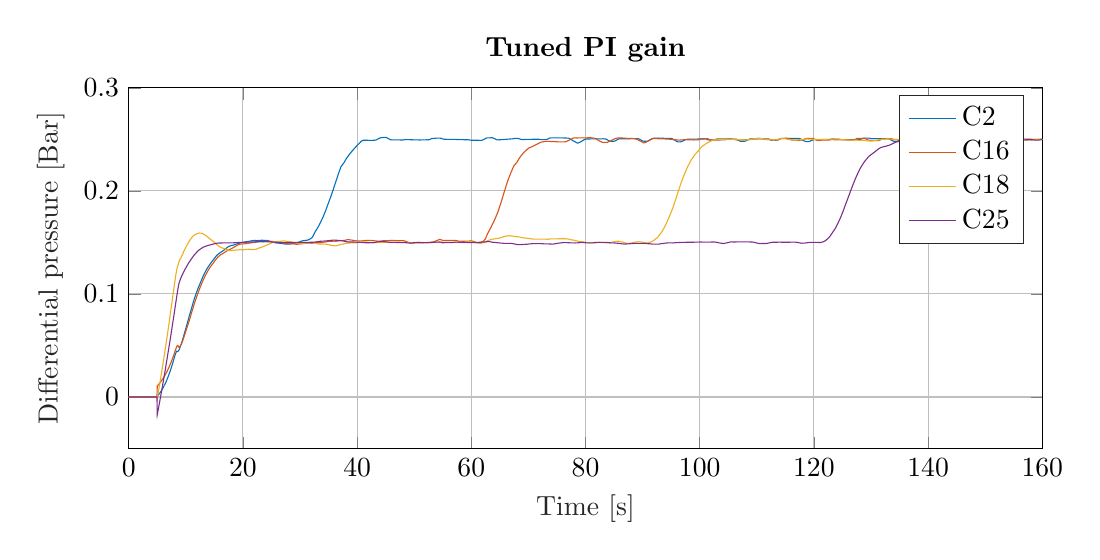
\begin{tikzpicture}

\begin{axis}[%
width=4.568in,
height=1.803in,
at={(0.766in,0.486in)},
scale only axis,
xmin=0,
xmax=160,
xlabel style={font=\color{white!15!black}},
xlabel={Time [s]},
ymin=-0.05,
ymax=0.3,
ylabel style={font=\color{white!15!black}},
ylabel={Differential pressure [Bar]},
axis background/.style={fill=white},
title style={font=\bfseries},
title={Tuned PI gain},
xmajorgrids,
ymajorgrids,
legend style={legend cell align=left, align=left, draw=white!15!black}
]
\addplot [color=mycolor1]
  table[row sep=crcr]{%
0	0\\
4.94999999999999	0\\
5	0.000684261974583933\\
5.5	0.00411168132941953\\
5.80000000000001	0.00671432062560484\\
6.05000000000001	0.00924364613879902\\
6.5	0.014082355816214\\
6.65000000000001	0.0160496089931712\\
7.05000000000001	0.0217925219941435\\
7.40000000000001	0.027346041055722\\
7.65000000000001	0.0317754154447698\\
8	0.0384042033235517\\
8.15000000000001	0.0411351417399715\\
8.34999999999999	0.0440127077223735\\
8.40000000000001	0.0443365102639177\\
8.55000000000001	0.0440188172042895\\
8.59999999999999	0.0441532258064399\\
8.80000000000001	0.04550342130986\\
8.84999999999999	0.0460716031280413\\
9.05000000000001	0.0489980449657992\\
9.34999999999999	0.0539711632453646\\
9.5	0.0567265395894481\\
10.4	0.0742974095796569\\
10.6	0.0783235581622819\\
11.35	0.0927724828934515\\
11.55	0.0963404203323535\\
11.7	0.0986375855327424\\
12.05	0.104026148582591\\
12.35	0.108162267839674\\
12.55	0.110807673509299\\
13	0.116746089931581\\
13.2	0.119214320625616\\
13.45	0.121890273704793\\
13.75	0.124871700879766\\
14.1	0.127779814271747\\
14.45	0.130504643206251\\
15.35	0.136992913000967\\
15.55	0.138019305962843\\
15.9	0.139626099706732\\
16.15	0.140585288367532\\
16.45	0.141611681329437\\
17	0.143811094819171\\
17.35	0.145515640273715\\
17.45	0.145967741935493\\
17.8	0.146713098729236\\
18.05	0.146981915933537\\
18.25	0.147220185728258\\
18.6	0.147898338220926\\
19.05	0.148771994134904\\
19.35	0.149205767350935\\
19.65	0.1497678396872\\
21.05	0.151087487781041\\
21.95	0.151991691104598\\
22.1	0.151930596285439\\
22.3	0.151802297165204\\
22.65	0.15180840664712\\
23.35	0.152126099706749\\
24	0.151845063538616\\
24.3	0.151851173020532\\
24.95	0.150641495601178\\
25.15	0.150256598240475\\
25.35	0.149975562072342\\
25.6	0.1497678396872\\
25.95	0.149395161290329\\
26.1	0.14930351906159\\
26.3	0.149266862170094\\
27.45	0.148411534701864\\
27.7	0.14847873900294\\
27.95	0.148374877810369\\
28.2	0.148484848484856\\
28.6	0.148857526881727\\
29	0.149028592375373\\
29.3	0.149260752688178\\
29.95	0.150568181818187\\
30.4	0.151551808406651\\
30.85	0.151875610948196\\
31.2	0.152126099706749\\
31.45	0.152468230694041\\
31.65	0.152950879765399\\
31.85	0.153616813294235\\
32.15	0.154875366568916\\
32.2	0.155241935483872\\
32.45	0.15796065493646\\
32.65	0.160270039100681\\
33.1	0.164271749755613\\
33.55	0.169006598240458\\
34.05	0.174816715542534\\
34.4	0.179588220918873\\
34.75	0.184872922776151\\
35.15	0.19086021505376\\
35.35	0.193719452590415\\
35.8	0.200995845552285\\
36.75	0.216947702834801\\
37.15	0.22313049853372\\
37.2	0.223723118279565\\
37.45	0.225617057673503\\
37.65	0.226936705767343\\
38.1	0.231237781036157\\
38.5	0.23438416422286\\
39.1	0.238508064516139\\
39.55	0.241379521016626\\
40	0.243976050830895\\
40.7	0.248063294232651\\
40.8	0.24848484848485\\
41.05	0.249150782013686\\
42.7	0.249077468230695\\
43	0.249169110459434\\
43.25	0.249285190615836\\
43.4	0.249645650048876\\
44	0.251435728250243\\
44.35	0.251759530791787\\
44.6	0.251808406647115\\
44.85	0.251942815249265\\
45.1	0.25187561094819\\
45.2	0.251576246334309\\
45.4	0.250879765395894\\
45.85	0.249682306940372\\
46.1	0.249456256109482\\
46.7	0.249566226783969\\
46.95	0.249560117302053\\
47.25	0.249578445747801\\
47.4	0.249529569892474\\
47.7	0.249370723362659\\
48.05	0.249401270772239\\
48.3	0.249828934506354\\
48.5	0.249847262952102\\
50.25	0.249517350928642\\
50.4	0.249566226783969\\
50.9	0.249425708699903\\
52.2	0.249615102639297\\
52.4	0.249584555229717\\
52.6	0.249676197458456\\
52.9	0.250378787878788\\
53.05	0.250818670576734\\
53.3	0.250928641251221\\
53.45	0.250922531769305\\
53.7	0.251111925708699\\
53.85	0.251203567937438\\
54.25	0.251228005865102\\
54.5	0.251191348973606\\
54.7	0.251075268817203\\
55	0.250421554252199\\
55.1	0.250213831867057\\
55.65	0.250073313782991\\
56.6	0.250067204301075\\
58.85	0.249663978494624\\
59.05	0.249657869012708\\
59.4	0.249725073313783\\
60.05	0.249108015640275\\
60.6	0.249169110459434\\
60.85	0.249169110459434\\
61.8	0.249053030303031\\
61.95	0.249297409579668\\
62.7	0.251374633431084\\
62.9	0.251521260997066\\
63.2	0.25151515151515\\
63.7	0.251582355816225\\
63.8	0.251435728250243\\
64.15	0.250519305962854\\
64.4	0.249786168132943\\
64.6	0.249523460410558\\
65.25	0.249725073313783\\
67.2	0.250537634408602\\
67.6	0.250904203323557\\
68.2	0.250971407624633\\
68.35	0.2506903714565\\
68.8	0.249816715542522\\
69	0.249853372434018\\
69.2	0.249871700879766\\
69.5	0.249945014662757\\
70.5	0.250073313782991\\
71.85	0.250128299120234\\
71.95	0.249975562072336\\
72.1	0.249731182795699\\
72.35	0.249725073313783\\
72.75	0.249743401759531\\
73.25	0.249908357771261\\
73.7	0.251282991202345\\
73.95	0.251466275659823\\
75.25	0.25151515151515\\
75.6	0.25151515151515\\
77	0.251234115347017\\
77.1	0.251111925708699\\
77.35	0.250274926686217\\
77.7	0.249101906158359\\
78.55	0.24647482893451\\
78.7	0.24647482893451\\
79.15	0.247623411534704\\
79.75	0.249621212121212\\
79.95	0.250201612903226\\
80.05	0.250397116324535\\
80.65	0.250415444770283\\
81.7	0.250500977517106\\
81.9	0.250604838709677\\
82.2	0.250476539589442\\
83.1	0.250580400782013\\
83.55	0.25036045943304\\
83.8	0.249608993157381\\
84.05	0.248808651026394\\
84.35	0.248081622678427\\
84.5	0.248026637341184\\
85.1	0.248289345063569\\
85.6	0.249798387096803\\
85.8	0.250391006842648\\
85.95	0.250598729227789\\
86.2	0.250592619745873\\
88.8	0.250720918866136\\
88.95	0.25077590420338\\
89.3	0.250519305962911\\
89.45	0.250213831867114\\
89.7	0.249431818181876\\
90.05	0.248350439882756\\
90.3	0.248130498533783\\
90.85	0.248258797654017\\
90.95	0.248448191593411\\
91.15	0.249132453567995\\
91.65	0.250757575757632\\
92	0.251166911045999\\
92.25	0.251203567937495\\
92.6	0.251252443792822\\
92.8	0.25130131964815\\
94.1	0.250946969697026\\
95.05	0.25091031280553\\
95.5	0.249682306940429\\
95.75	0.248906402737106\\
95.95	0.248106060606119\\
96.15	0.247653958944341\\
96.25	0.247617302052845\\
96.45	0.247623411534761\\
96.6	0.24751955034219\\
96.85	0.247916666666725\\
97.25	0.248967497556265\\
97.6	0.249865591397906\\
97.8	0.250097751710712\\
98.3	0.250164956011787\\
99.4	0.250305474095853\\
100.7	0.250427663734172\\
101	0.250629276637397\\
101.2	0.250342130987349\\
101.4	0.249627321603185\\
101.7	0.24942570869996\\
102.5	0.249541788856362\\
102.7	0.249792277614915\\
102.85	0.250097751710712\\
103	0.250476539589499\\
104	0.250476539589499\\
104.45	0.250421554252256\\
104.85	0.250391006842676\\
105.1	0.25041544477034\\
105.95	0.250287145650105\\
106.25	0.250268817204358\\
106.45	0.250128299120291\\
106.65	0.249578445747858\\
107	0.248350439882756\\
107.1	0.248234359726354\\
107.45	0.248222140762522\\
107.6	0.248191593352942\\
107.75	0.248130498533783\\
108.05	0.248429863147663\\
108.4	0.249456256109539\\
108.7	0.250274926686274\\
108.95	0.250391006842676\\
109.95	0.250525415444827\\
110.3	0.250476539589499\\
111.3	0.250470430107583\\
111.85	0.250525415444827\\
112.05	0.25054985337249\\
112.4	0.249499022482951\\
112.5	0.249187438905238\\
112.75	0.249254643206314\\
113	0.249327956989305\\
113.25	0.249193548387154\\
113.65	0.249315738025473\\
113.95	0.250207722385198\\
114.05	0.250543743890574\\
114.25	0.250739247311884\\
114.45	0.25087976539595\\
115.3	0.250965298142773\\
117.5	0.250928641251278\\
117.75	0.250171065493703\\
118	0.249315738025473\\
118.2	0.248765884653039\\
118.5	0.24804496578696\\
118.8	0.247794477028407\\
119.15	0.247861681329482\\
119.6	0.249004154447761\\
120.1	0.249975562072393\\
120.3	0.249871700879822\\
120.8	0.24969452590426\\
121.2	0.249798387096831\\
121.45	0.249871700879822\\
121.9	0.249853372434075\\
122.15	0.249945014662813\\
122.75	0.249902248289402\\
123.25	0.250030547409636\\
124.35	0.249877810361738\\
124.55	0.249828934506411\\
124.85	0.249718963831924\\
127.95	0.249835043988327\\
128.15	0.250091642228796\\
128.45	0.250855327468287\\
128.75	0.251154692082167\\
129.2	0.251209677419411\\
129.5	0.251289100684318\\
129.7	0.251252443792822\\
129.85	0.250995845552353\\
130	0.250708699902304\\
130.3	0.250800342131043\\
130.55	0.250739247311884\\
131.65	0.250720918866136\\
132.3	0.250769794721464\\
132.5	0.250720918866136\\
132.8	0.250812561094875\\
133.05	0.250629276637397\\
133.15	0.250500977517163\\
134.1	0.247776148582659\\
134.3	0.2477150537635\\
134.45	0.247745601173079\\
134.6	0.247696725317752\\
134.75	0.247782258064575\\
135.4	0.24975562072342\\
135.55	0.249981671554309\\
135.65	0.25008553274688\\
136.55	0.249993890518141\\
137.25	0.249975562072393\\
137.9	0.249773949169168\\
138.45	0.249780058651083\\
138.75	0.249780058651083\\
138.9	0.249963343108561\\
139.1	0.250207722385198\\
139.45	0.250207722385198\\
139.95	0.25021994134903\\
140.55	0.250201612903282\\
141.1	0.25008553274688\\
141.85	0.249749511241504\\
142.3	0.249706744868092\\
142.6	0.249847262952159\\
142.8	0.249773949169168\\
143.1	0.249676197458513\\
143.6	0.249523460410614\\
144.1	0.250189393939451\\
144.8	0.250048875855384\\
145.35	0.250006109481973\\
145.8	0.249938905180898\\
146.85	0.250336021505433\\
147.35	0.250274926686274\\
148.65	0.250171065493703\\
149.1	0.249499022482951\\
149.7	0.249663978494681\\
150.45	0.249835043988327\\
150.65	0.250244379276694\\
150.85	0.250488758553331\\
151.1	0.250378787878844\\
152.2	0.250800342131043\\
152.85	0.250769794721464\\
153.3	0.250812561094875\\
153.85	0.2507453567938\\
154.1	0.250311583577769\\
154.75	0.248588709677477\\
155.7	0.248680351906216\\
155.85	0.248930840664769\\
156.1	0.249749511241504\\
156.5	0.24972507331384\\
157	0.249523460410614\\
158	0.249639540567017\\
158.75	0.249786168132999\\
159.6	0.250000000000057\\
159.7	0.250146627566039\\
160.5	0.250079423264964\\
160.7	0.2500549853373\\
};
\addlegendentry{C2}

\addplot [color=mycolor2]
  table[row sep=crcr]{%
0	0\\
4.94999999999999	0\\
5	0.0106182795698828\\
5.25	0.0121700879765285\\
5.90000000000001	0.0169843597263082\\
6.19999999999999	0.0195625610948298\\
6.65000000000001	0.0240285923753731\\
7	0.0280608504398856\\
7.15000000000001	0.030058651026394\\
7.34999999999999	0.0327468230694024\\
7.5	0.0347568426197427\\
7.80000000000001	0.0392778592375294\\
8.30000000000001	0.0472812805474234\\
8.34999999999999	0.0480632942326622\\
8.40000000000001	0.0486803519061709\\
8.55000000000001	0.0500794232649184\\
8.59999999999999	0.0500610948191706\\
8.80000000000001	0.0480510752688303\\
8.84999999999999	0.0480205278592507\\
9.15000000000001	0.0506414956011838\\
9.30000000000001	0.0521627565982499\\
9.5	0.0552969208211209\\
9.80000000000001	0.0602333822091907\\
10.2	0.0672592864125079\\
10.4	0.0705950635386046\\
10.5	0.0723301564027281\\
10.75	0.0768572825024307\\
11.05	0.0824474584555333\\
11.45	0.0897421798631513\\
11.7	0.0939943792766371\\
12.1	0.100219941348968\\
12.5	0.106353861192559\\
12.85	0.111052052785936\\
13.25	0.115957966764427\\
13.45	0.118175708699908\\
13.75	0.121389296187687\\
14.05	0.124211876832845\\
14.3	0.126228005865102\\
14.7	0.129142228738999\\
14.95	0.131133919843592\\
15.2	0.133064516129025\\
15.5	0.135062316715533\\
15.9	0.137261730205267\\
16.15	0.138141495601161\\
16.35	0.138734115347006\\
17.15	0.141648338220932\\
17.45	0.142381476050844\\
18.15	0.144477028348007\\
19.1	0.147507331378307\\
19.45	0.148216031280555\\
19.75	0.148552052785931\\
20.3	0.148631476050838\\
20.65	0.149028592375373\\
20.95	0.149150782013692\\
21.45	0.149645650048882\\
21.7	0.149792277614864\\
22.85	0.150659824046926\\
23.15	0.150708699902253\\
23.7	0.150672043010758\\
23.9	0.150733137829917\\
24.3	0.150898093841647\\
24.75	0.151118035190621\\
25.3	0.150995845552302\\
27.3	0.149407380254161\\
27.65	0.148894183773223\\
27.85	0.148680351906165\\
28.05	0.148552052785931\\
28.7	0.148686461388081\\
29.05	0.148411534701864\\
29.3	0.148228250244387\\
29.6	0.148271016617798\\
31.35	0.149444037145656\\
31.65	0.149327956989254\\
32.05	0.149181329423271\\
32.55	0.149596774193554\\
32.9	0.14993279569893\\
33.05	0.149853372434023\\
33.25	0.149621212121218\\
33.5	0.149639540566966\\
34.2	0.150274926686222\\
34.7	0.150708699902253\\
35	0.15098362658847\\
35.15	0.151050830889545\\
35.55	0.151118035190621\\
35.9	0.151228005865107\\
36.25	0.151099706744873\\
36.7	0.151411290322585\\
36.9	0.151606793743895\\
37.45	0.151759530791793\\
37.7	0.151936705767355\\
37.85	0.152010019550346\\
38.3	0.152675953079182\\
38.6	0.152627077223855\\
39.35	0.151948924731187\\
39.6	0.151710654936466\\
39.75	0.151606793743895\\
39.9	0.151490713587492\\
40.25	0.151484604105576\\
40.55	0.151454056695997\\
40.75	0.151423509286417\\
41.3	0.151790078201373\\
41.75	0.151918377321607\\
42.35	0.152046676441842\\
43.7	0.151154692082116\\
44.85	0.151759530791793\\
45.55	0.151783968719457\\
45.7	0.151857282502448\\
46.1	0.15180840664712\\
46.45	0.151832844574784\\
47.4	0.151728983382213\\
47.8	0.151771749755625\\
48.3	0.151521260997072\\
48.8	0.150452101661784\\
49.05	0.149835043988276\\
49.35	0.149376832844581\\
49.65	0.149297409579674\\
50	0.149480694037152\\
50.2	0.149560117302059\\
50.9	0.149523460410563\\
51.45	0.149584555229723\\
52	0.149859481915939\\
53	0.14982893450636\\
53.25	0.150164956011736\\
54.4	0.152785923753669\\
54.55	0.152785923753669\\
54.65	0.15266373411535\\
54.95	0.152046676441842\\
55.3	0.151845063538616\\
56.75	0.151918377321607\\
57.1	0.151845063538616\\
57.35	0.151820625610952\\
57.5	0.151606793743895\\
57.7	0.151276881720435\\
58.65	0.151160801564032\\
59.15	0.151240224828939\\
59.3	0.151209677419359\\
60.05	0.151490713587492\\
60.2	0.151307429130014\\
60.55	0.150580400782019\\
60.9	0.149890029325519\\
61.2	0.149431818181824\\
61.35	0.149370723362665\\
61.55	0.149725073313789\\
62.1	0.151221896383191\\
62.2	0.151631231671558\\
62.4	0.152908113391987\\
62.45	0.153323558162271\\
62.55	0.154563782991204\\
62.75	0.15723973607038\\
62.9	0.15914589442815\\
63.05	0.160575513196477\\
63.45	0.164693304007812\\
64.05	0.17156647116326\\
64.5	0.177394916911055\\
64.65	0.17953323558163\\
64.8	0.181860948191598\\
65.25	0.189497800586508\\
65.75	0.198723118279588\\
66.15	0.205901759530803\\
66.4	0.210019550342139\\
66.65	0.213697458455528\\
67	0.218542277614858\\
67.3	0.222458455522968\\
67.45	0.224224095796671\\
67.55	0.225012218963855\\
67.95	0.227431573802562\\
68.45	0.232080889540583\\
68.7	0.234023704789848\\
69.3	0.237897116324547\\
69.6	0.239461143695024\\
70.1	0.241678885630506\\
70.35	0.242289833822099\\
70.5	0.242607526881727\\
72.15	0.247140762463346\\
72.7	0.247837243401761\\
72.85	0.247983870967744\\
73	0.24812438905181\\
74.2	0.247941104594332\\
74.6	0.247934995112416\\
75.2	0.247605083088956\\
76	0.24762952101662\\
76.2	0.247580645161293\\
76.35	0.24762952101662\\
76.55	0.247757820136854\\
76.75	0.248173264907138\\
77.85	0.251270772238513\\
78.05	0.251472385141739\\
78.25	0.251411290322579\\
78.45	0.251344086021504\\
78.7	0.251423509286411\\
79.2	0.25148460410557\\
79.45	0.251502932551318\\
80.95	0.251564027370478\\
81.6	0.251130254154447\\
81.8	0.250629276637341\\
82.3	0.24897971652004\\
82.45	0.248478739002934\\
82.95	0.247079667644186\\
83.2	0.247006353861195\\
83.4	0.24710410557185\\
83.85	0.247152981427178\\
84.65	0.249224095796677\\
85.3	0.251038611925708\\
85.65	0.251337976539588\\
86	0.251423509286411\\
86.2	0.251429618768327\\
87.7	0.25082478005865\\
88	0.250940860215053\\
88.55	0.250647605083088\\
88.75	0.250543743890518\\
88.95	0.250171065493646\\
89.2	0.249511241446726\\
90.15	0.246725317693063\\
90.25	0.246584799608996\\
90.45	0.246859726295213\\
91.7	0.250574291300097\\
92.05	0.250873655913978\\
92.35	0.250782013685239\\
93.3	0.250433773216031\\
93.5	0.250507086999022\\
93.9	0.250427663734115\\
94.2	0.250372678396872\\
94.7	0.250183284457478\\
95.25	0.249859481915934\\
95.4	0.24970063538612\\
95.65	0.24967008797654\\
95.95	0.249566226783969\\
96.35	0.249272971652033\\
96.55	0.249309628543529\\
97.25	0.249718963831896\\
97.45	0.249718963831896\\
97.85	0.249694525904232\\
98.5	0.249584555229774\\
98.85	0.249456256109539\\
99.7	0.249468475073371\\
100	0.249981671554309\\
100.2	0.250458211143751\\
100.35	0.250702590420389\\
101.1	0.250635386119313\\
101.4	0.25058040078207\\
101.55	0.250342130987349\\
101.75	0.249657869012765\\
102	0.249431818181876\\
102.3	0.249389051808464\\
102.65	0.24942570869996\\
103.2	0.249456256109539\\
103.5	0.249431818181876\\
103.9	0.249499022482951\\
104.55	0.249682306940429\\
104.7	0.250103861192628\\
105	0.25041544477034\\
106	0.249908357771318\\
106.2	0.249816715542579\\
106.55	0.249382942326548\\
106.8	0.249468475073371\\
108	0.24959066471169\\
108.65	0.249865591397906\\
108.95	0.24992057673515\\
109.2	0.250042766373468\\
109.35	0.250213831867114\\
109.65	0.250604838709734\\
110.15	0.250678152492725\\
110.4	0.250672043010809\\
110.95	0.2507453567938\\
111.6	0.249865591397906\\
112.45	0.24975562072342\\
112.75	0.249645650048933\\
112.95	0.249554007820194\\
113.1	0.249474584555287\\
113.6	0.249517350928699\\
113.75	0.249663978494681\\
114.2	0.250818670576791\\
115.05	0.251111925708756\\
115.25	0.251093597263008\\
115.4	0.250928641251278\\
115.65	0.250525415444827\\
116.05	0.249474584555287\\
116.3	0.249291300097809\\
116.75	0.249272971652061\\
117.05	0.249138563049911\\
117.25	0.249144672531827\\
117.7	0.249242424242482\\
117.95	0.249291300097809\\
118.25	0.249969452590477\\
118.45	0.250488758553331\\
118.7	0.250946969697026\\
118.9	0.250989736070437\\
119.8	0.250873655914035\\
120.5	0.249175219941407\\
120.6	0.24903470185734\\
121.55	0.24926075268823\\
122.65	0.2493646138808\\
122.8	0.249810606060663\\
122.9	0.250103861192628\\
123.15	0.250391006842676\\
124.55	0.250146627566039\\
124.9	0.249541788856362\\
125.05	0.249505131964867\\
125.8	0.249468475073371\\
126.1	0.249334066471221\\
126.5	0.249358504398884\\
127	0.249407380254212\\
127.1	0.249584555229774\\
127.4	0.250519305962911\\
127.55	0.25094086021511\\
127.7	0.250965298142773\\
127.85	0.250867546432119\\
128.35	0.250898093841698\\
128.55	0.250855327468287\\
128.85	0.250861436950203\\
129	0.25071480938422\\
129.2	0.250268817204358\\
129.55	0.249315738025473\\
129.85	0.248973607038181\\
130.55	0.248949169110517\\
130.8	0.248857526881778\\
131.1	0.248906402737106\\
131.25	0.248894183773274\\
131.45	0.249022482893508\\
131.85	0.250152737047955\\
132.1	0.250562072336322\\
132.55	0.250464320625667\\
132.8	0.250727028348052\\
133.5	0.250782013685296\\
134.05	0.249633431085101\\
134.15	0.249535679374446\\
134.85	0.249578445747858\\
135.2	0.249663978494681\\
135.85	0.249896138807486\\
136.05	0.249816715542579\\
136.35	0.250128299120291\\
136.45	0.250323802541601\\
136.65	0.250366568915013\\
137	0.250433773216088\\
137.6	0.250336021505433\\
138	0.250256598240526\\
138.45	0.250024437927721\\
138.7	0.249682306940429\\
138.85	0.249566226784026\\
140.2	0.249615102639353\\
140.45	0.249608993157437\\
140.65	0.249828934506411\\
140.85	0.250421554252256\\
141.15	0.251344086021561\\
141.3	0.251625122189694\\
142.05	0.251655669599273\\
142.25	0.25163123167161\\
142.4	0.251472385141795\\
142.5	0.251325757575813\\
143.1	0.249676197458513\\
143.45	0.248918621700938\\
143.7	0.248949169110517\\
144.2	0.249144672531827\\
144.5	0.249163000977575\\
145.05	0.249584555229774\\
145.6	0.25107526881726\\
145.75	0.251136363636419\\
146.1	0.251124144672588\\
146.45	0.250843108504455\\
146.7	0.250122189638375\\
147.1	0.248930840664769\\
147.25	0.248533724340234\\
147.6	0.248148826979531\\
148	0.248099951124203\\
148.25	0.247996089931632\\
148.55	0.248442082111495\\
149.2	0.250232160312862\\
149.45	0.250965298142773\\
149.8	0.251985581622733\\
149.95	0.252358260019605\\
150.05	0.252382697947269\\
150.3	0.251997800586565\\
150.55	0.251154692082167\\
150.75	0.250604838709734\\
151.4	0.24890029325519\\
152.35	0.248790322580703\\
152.6	0.248912512219022\\
152.9	0.249737292277672\\
153.3	0.250977517106605\\
153.45	0.251246334310906\\
154.5	0.251142473118335\\
154.65	0.250946969697026\\
155.1	0.249615102639353\\
155.3	0.249334066471221\\
155.55	0.24942570869996\\
156	0.249303519061641\\
156.35	0.249272971652061\\
156.6	0.249169110459491\\
157.3	0.2493646138808\\
157.5	0.249615102639353\\
157.6	0.249816715542579\\
157.95	0.249877810361738\\
158.4	0.249767839687252\\
158.8	0.249798387096831\\
160.1	0.249767839687252\\
160.7	0.249743401759588\\
};
\addlegendentry{C16}

\addplot [color=mycolor3]
  table[row sep=crcr]{%
0	0\\
4.94999999999999	0\\
5	-0.0012891006842608\\
5.5	0.0150048875855191\\
5.84999999999999	0.0268572825024478\\
6.25	0.0410129521016529\\
6.65000000000001	0.0556573802541607\\
6.94999999999999	0.0672226295210123\\
7.44999999999999	0.0868523949169173\\
7.75	0.0989980449657821\\
8.15000000000001	0.114839931573812\\
8.19999999999999	0.116654447702842\\
8.40000000000001	0.123258797653961\\
8.44999999999999	0.124578445747801\\
8.84999999999999	0.132050342130981\\
8.90000000000001	0.132704056695985\\
9.09999999999999	0.134457478005857\\
9.19999999999999	0.135538856304976\\
9.40000000000001	0.138031524926674\\
9.75	0.142662512218976\\
9.90000000000001	0.14423264907137\\
10.45	0.149712854349957\\
10.7	0.151979472140766\\
10.85	0.153176930596288\\
11.1	0.155076979472142\\
11.2	0.155816226783969\\
11.35	0.156537145650049\\
11.65	0.157746823069402\\
12.2	0.158907624633429\\
12.35	0.159109237536654\\
12.7	0.158962609970672\\
12.9	0.158657135874876\\
13.25	0.157557429130009\\
13.75	0.155663489736071\\
14.15	0.153824535679377\\
14.7	0.151411290322585\\
14.9	0.150672043010758\\
15.3	0.148619257087006\\
15.55	0.147305718475081\\
15.8	0.146230449657878\\
16.15	0.145075757575768\\
16.55	0.144312072336277\\
17.2	0.143157380254166\\
17.6	0.142198191593366\\
17.85	0.14196603128056\\
18.2	0.142216520039113\\
18.8	0.142613636363649\\
19.25	0.142741935483883\\
19.5	0.143041300097764\\
20	0.142754154447715\\
20.2	0.142949657869025\\
20.5	0.143187927663746\\
21.05	0.143383431085056\\
21.35	0.143139051808419\\
22.05	0.143169599217998\\
22.3	0.143358993157392\\
22.7	0.144342619745856\\
23.3	0.145332355816237\\
23.55	0.14594330400783\\
24.4	0.147825024437935\\
24.55	0.1481182795699\\
24.85	0.149120234604112\\
25.4	0.150543743890523\\
25.55	0.150733137829917\\
25.7	0.150812561094824\\
26	0.150861436950152\\
26.25	0.151001955034218\\
26.5	0.151087487781041\\
27.15	0.151441837732165\\
27.25	0.151447947214081\\
27.65	0.151026392961882\\
28.05	0.15081867057674\\
28.2	0.150763685239497\\
28.5	0.15035434995113\\
28.85	0.149853372434023\\
29.3	0.149315738025422\\
29.5	0.149083577712616\\
29.85	0.148814760508316\\
30	0.148771994134904\\
30.25	0.148686461388081\\
31	0.149535679374395\\
31.2	0.149816715542528\\
31.8	0.149786168132948\\
32.4	0.14946847507332\\
32.55	0.149517350928647\\
32.8	0.149034701857289\\
33.05	0.148820869990232\\
33.25	0.148490957966771\\
34.15	0.148380987292285\\
34.4	0.14841764418378\\
35	0.14778836754644\\
35.45	0.147146871945267\\
36.3	0.146645894428161\\
36.85	0.147568426197466\\
37.35	0.148393206256117\\
37.55	0.148405425219948\\
37.75	0.148802541544484\\
38	0.148991935483878\\
38.15	0.149150782013692\\
38.3	0.149340175953085\\
38.65	0.149419599217993\\
39.45	0.149725073313789\\
39.6	0.149725073313789\\
39.8	0.149670087976546\\
40.25	0.149792277614864\\
40.9	0.150555962854355\\
41.05	0.150617057673514\\
41.65	0.15035434995113\\
42	0.150024437927669\\
42.5	0.149566226783975\\
42.95	0.149627321603134\\
43.5	0.149914467253183\\
43.6	0.149975562072342\\
43.75	0.150006109481922\\
44.25	0.150109970674492\\
44.55	0.149975562072342\\
45.05	0.150164956011736\\
45.25	0.150073313782997\\
45.65	0.149835043988276\\
46.05	0.149865591397855\\
46.4	0.150018328445753\\
46.8	0.150091642228745\\
47.2	0.150226050830895\\
47.65	0.150189393939399\\
47.8	0.150054985337249\\
47.95	0.149938905180846\\
48.3	0.150012218963838\\
48.5	0.149883919843603\\
48.6	0.149780058651032\\
48.9	0.149725073313789\\
49.35	0.14963343108505\\
49.65	0.149474584555236\\
49.8	0.149547898338227\\
50.5	0.150189393939399\\
51.15	0.150073313782997\\
51.4	0.149981671554258\\
51.8	0.149792277614864\\
52	0.149590664711639\\
52.2	0.149572336265891\\
52.45	0.149578445747807\\
52.8	0.149670087976546\\
52.95	0.149957233626594\\
53.5	0.150018328445753\\
53.8	0.150079423264913\\
54.5	0.150195503421315\\
54.75	0.150238269794727\\
55.05	0.150103861192576\\
56.55	0.150018328445753\\
56.75	0.150091642228745\\
57.1	0.149951124144678\\
57.85	0.149926686217015\\
58	0.149908357771267\\
58.2	0.149908357771267\\
58.4	0.1497678396872\\
58.8	0.149896138807435\\
59.05	0.150207722385147\\
59.6	0.150690371456506\\
59.9	0.150641495601178\\
61.15	0.149382942326497\\
61.7	0.149144672531776\\
61.9	0.149425708699908\\
62.55	0.150702590420337\\
62.75	0.151466275659828\\
62.85	0.151716764418381\\
63.15	0.15219941348974\\
63.45	0.152773704789837\\
63.7	0.153201368523952\\
64.2	0.153512952101664\\
64.5	0.153787878787881\\
64.95	0.1541788856305\\
65.15	0.15456989247312\\
65.35	0.154979227761487\\
65.6	0.155382453567938\\
65.85	0.155846774193549\\
66.45	0.156500488758553\\
66.75	0.156378299120234\\
67.65	0.155846774193549\\
67.85	0.155547409579668\\
68.25	0.155406891495602\\
68.35	0.155400782013686\\
68.95	0.154576001955036\\
69.85	0.153934506353863\\
70.1	0.153787878787881\\
70.9	0.153213587487784\\
71.55	0.15315860215054\\
71.95	0.153231915933532\\
72.15	0.153140273704793\\
73.1	0.153128054740961\\
73.4	0.153073069403717\\
73.75	0.153360215053766\\
74.45	0.153402981427178\\
74.65	0.153482404692085\\
74.95	0.153445747800589\\
75.2	0.153494623655916\\
75.55	0.153604594330403\\
76.2	0.153574046920824\\
76.55	0.153537390029328\\
77.1	0.153195259042036\\
77.35	0.15269428152493\\
77.5	0.152535434995116\\
77.85	0.152278836754647\\
78.7	0.151142473118284\\
79.6	0.150464320625616\\
80	0.150036656891501\\
80.65	0.149682306940377\\
81	0.149486803519068\\
82.05	0.149682306940377\\
82.45	0.150171065493652\\
82.6	0.150067204301081\\
82.8	0.149859481915939\\
84.25	0.149456256109488\\
84.55	0.149902248289351\\
84.8	0.150421554252205\\
85.4	0.151032502443798\\
85.8	0.151173020527864\\
86.1	0.150806451612908\\
86.5	0.15035434995113\\
86.85	0.149731182795705\\
87.15	0.149389051808413\\
87.4	0.149010263929625\\
87.6	0.149034701857289\\
88	0.149376832844581\\
88.6	0.150201612903231\\
89.25	0.150641495601178\\
89.5	0.150555962854355\\
89.95	0.150281036168138\\
90.6	0.149486803519068\\
90.85	0.149578445747807\\
91.5	0.150531524926691\\
91.8	0.151411290322585\\
92.1	0.1525293255132\\
92.5	0.154331622678399\\
92.7	0.155449657869013\\
93.25	0.159316959921796\\
93.5	0.161424731182791\\
93.65	0.162921554252193\\
93.95	0.166202346041047\\
94.2	0.169006598240458\\
94.35	0.170845552297152\\
94.95	0.17864736070382\\
95.2	0.182148093841647\\
95.4	0.185184506353863\\
95.65	0.189479472140761\\
95.95	0.194489247311822\\
96.4	0.202168866080143\\
96.85	0.209494134897369\\
97	0.211663000977524\\
97.3	0.215774682306943\\
97.45	0.217986314760509\\
97.7	0.221260997067446\\
98.15	0.226160801564021\\
98.35	0.228329667644175\\
98.55	0.230333577712628\\
99.2	0.235538856304998\\
99.5	0.237353372434029\\
99.75	0.238770772238524\\
100.15	0.241611681329431\\
100.45	0.243255131964816\\
101.05	0.245631720430111\\
101.3	0.246450391006846\\
102.25	0.249163000977518\\
103.05	0.250226050830889\\
103.4	0.250091642228739\\
103.75	0.250177174975562\\
104.05	0.250171065493646\\
104.55	0.250152737047898\\
104.75	0.250219941348973\\
105.05	0.249993890518084\\
105.3	0.250097751710655\\
105.6	0.250042766373411\\
105.85	0.250036656891496\\
107.95	0.249364613880772\\
108.7	0.249914467253234\\
109.1	0.24992057673515\\
110.05	0.251111925708756\\
110.35	0.251093597263008\\
110.55	0.25110581622684\\
111.25	0.250378787878844\\
111.55	0.250128299120291\\
111.85	0.249865591397906\\
112.35	0.249474584555287\\
112.7	0.249584555229774\\
112.85	0.249651759530849\\
113.15	0.249676197458513\\
113.7	0.250067204301132\\
114.1	0.250818670576791\\
114.8	0.250788123167212\\
115.05	0.250470430107583\\
115.45	0.249914467253234\\
116.85	0.249321847507389\\
117.45	0.249712854350008\\
117.75	0.249822825024495\\
118.75	0.25044599217992\\
119.05	0.250164956011787\\
119.3	0.250305474095853\\
119.85	0.250012218963889\\
120.1	0.249981671554309\\
120.6	0.249963343108561\\
120.9	0.249963343108561\\
122.1	0.24969452590426\\
122.5	0.249547898338278\\
123.3	0.249615102639353\\
123.65	0.249382942326548\\
124.45	0.249602883675522\\
124.85	0.249767839687252\\
126.6	0.249211876832902\\
126.85	0.249046920821172\\
127.15	0.249248533724398\\
127.5	0.249376832844632\\
128.1	0.248991935483929\\
128.3	0.249046920821172\\
128.5	0.249150782013743\\
128.75	0.248936950146685\\
128.9	0.248820869990283\\
129.1	0.248771994134955\\
129.4	0.24850928641257\\
130.15	0.248448191593411\\
131.7	0.249859481915991\\
131.9	0.250109970674544\\
132.3	0.250226050830946\\
133.15	0.250464320625667\\
133.6	0.250207722385198\\
133.85	0.250183284457535\\
134	0.250079423264964\\
134.15	0.249993890518141\\
134.4	0.250116080156459\\
134.7	0.249987781036225\\
135.75	0.250397116324592\\
136.05	0.250439882698004\\
136.6	0.250617057673566\\
136.75	0.25058040078207\\
136.95	0.25058040078207\\
137.35	0.25061094819165\\
137.75	0.25061094819165\\
137.95	0.250586510263986\\
138.2	0.25054985337249\\
138.7	0.250433773216088\\
139.3	0.250397116324592\\
139.5	0.25038489736076\\
139.85	0.250531524926743\\
140.5	0.25041544477034\\
140.7	0.250507086999079\\
143.25	0.250397116324592\\
143.5	0.25038489736076\\
144.45	0.250391006842676\\
145.2	0.250134408602207\\
145.45	0.250103861192628\\
145.6	0.2500549853373\\
145.9	0.250109970674544\\
146.45	0.250189393939451\\
146.75	0.250103861192628\\
147.45	0.249688416422345\\
147.8	0.249608993157437\\
148.1	0.24952956989253\\
149	0.249627321603185\\
149.15	0.249706744868092\\
149.35	0.249871700879822\\
149.7	0.249963343108561\\
149.9	0.250109970674544\\
150.45	0.250128299120291\\
150.7	0.250366568915013\\
151.5	0.24989002932557\\
151.8	0.249492913001035\\
152.05	0.249266862170145\\
152.35	0.248863636363694\\
152.65	0.248698680351964\\
152.8	0.248753665689208\\
153.3	0.249059139785004\\
153.55	0.249028592375424\\
153.75	0.249053030303088\\
153.9	0.249108015640331\\
154.15	0.24906524926692\\
156.2	0.248943059628601\\
156.5	0.249059139785004\\
157.5	0.250421554252256\\
157.75	0.250427663734172\\
159.4	0.250103861192628\\
159.6	0.250158846529871\\
159.8	0.25008553274688\\
160.1	0.250030547409636\\
160.45	0.250067204301132\\
160.7	0.250006109481973\\
};
\addlegendentry{C18}

\addplot [color=mycolor4]
  table[row sep=crcr]{%
0	0\\
4.94999999999999	0\\
5	-0.0172165200391134\\
5.19999999999999	-0.0113453079178782\\
5.55000000000001	-0.000788123167154708\\
6	0.0132636852394796\\
6.40000000000001	0.0262035679374435\\
7.34999999999999	0.058681573802545\\
7.94999999999999	0.0804374389051929\\
8.30000000000001	0.0934506353861195\\
8.40000000000001	0.0972018572824993\\
8.59999999999999	0.104191104594321\\
8.65000000000001	0.105761241446714\\
8.80000000000001	0.110080645161304\\
8.84999999999999	0.111186461388087\\
9.25	0.117118768328453\\
9.34999999999999	0.118212365591404\\
9.55000000000001	0.120362903225811\\
9.80000000000001	0.123234359726297\\
10.1	0.126295210166177\\
10.3	0.128189149560114\\
10.5	0.130064760508304\\
10.75	0.132038123167149\\
10.95	0.133809872922768\\
11.45	0.137622189638307\\
11.75	0.139473362658833\\
11.95	0.140676930596271\\
12.1	0.141550586510277\\
12.3	0.142589198435985\\
13.05	0.145393450635396\\
13.4	0.146083822091896\\
13.55	0.146419843597272\\
13.7	0.146731427174984\\
15.25	0.149071358748785\\
15.5	0.149248533724347\\
15.8	0.149444037145656\\
17.9	0.149584555229723\\
18.3	0.149584555229723\\
18.75	0.14979838709678\\
19.85	0.150042766373417\\
20.05	0.150091642228745\\
20.25	0.150079423264913\\
20.95	0.150311583577718\\
21.4	0.150372678396877\\
21.65	0.150470430107532\\
22.1	0.150568181818187\\
22.45	0.150678152492674\\
22.8	0.150745356793749\\
24	0.150708699902253\\
24.15	0.150751466275665\\
24.7	0.150543743890523\\
24.9	0.150445992179868\\
26.95	0.149816715542528\\
28.75	0.149938905180846\\
29.25	0.149938905180846\\
29.55	0.149945014662762\\
31.45	0.150061094819165\\
31.65	0.150103861192576\\
32.05	0.150201612903231\\
32.3	0.150146627565988\\
32.65	0.150366568914961\\
32.85	0.150537634408607\\
33.05	0.150708699902253\\
33.2	0.150757575757581\\
33.5	0.151111925708705\\
34.35	0.151337976539594\\
34.9	0.151661779081138\\
35.65	0.152119990224833\\
35.9	0.152211632453572\\
36.3	0.15213831867058\\
36.8	0.151906158357775\\
37.15	0.151728983382213\\
37.35	0.151619012707727\\
37.65	0.151276881720435\\
37.8	0.151136363636368\\
38.05	0.150733137829917\\
38.25	0.15065371456501\\
38.5	0.150342130987298\\
38.9	0.150464320625616\\
39.2	0.150415444770289\\
40.1	0.150201612903231\\
40.4	0.150171065493652\\
41.3	0.149737292277621\\
41.85	0.149676197458462\\
42	0.149676197458462\\
42.25	0.149731182795705\\
42.6	0.149731182795705\\
42.95	0.149926686217015\\
43.3	0.150287145650054\\
43.6	0.150598729227767\\
44.6	0.150898093841647\\
45.15	0.150482649071364\\
45.8	0.150116080156408\\
46.3	0.150048875855333\\
47.65	0.149841153470192\\
48.25	0.149883919843603\\
48.45	0.149749511241453\\
49.55	0.14930351906159\\
50	0.149908357771267\\
50.3	0.149761730205284\\
50.95	0.149883919843603\\
51.75	0.149761730205284\\
52	0.149773949169116\\
52.75	0.150073313782997\\
52.95	0.150171065493652\\
53.25	0.150146627565988\\
53.6	0.150195503421315\\
53.8	0.150238269794727\\
54.5	0.150372678396877\\
54.7	0.15012829912024\\
54.95	0.149639540566966\\
55.4	0.14979838709678\\
56.3	0.149780058651032\\
56.8	0.149902248289351\\
57.1	0.150213831867063\\
57.45	0.150348240469214\\
58	0.150116080156408\\
58.25	0.150177174975568\\
58.55	0.150207722385147\\
59.35	0.149920576735099\\
59.55	0.14982893450636\\
60.15	0.149890029325519\\
60.3	0.149822825024444\\
62.4	0.150397116324541\\
62.6	0.150659824046926\\
63.05	0.150763685239497\\
63.25	0.150708699902253\\
63.7	0.150164956011736\\
64.25	0.149871700879771\\
64.55	0.149688416422293\\
65.25	0.149297409579674\\
65.5	0.149236314760515\\
65.8	0.149022482893457\\
67	0.149040811339205\\
67.65	0.148393206256117\\
67.8	0.148142717497564\\
68.2	0.147880009775179\\
68.35	0.147800586510272\\
69.8	0.148271016617798\\
70.15	0.148533724340183\\
70.7	0.148759775171072\\
72.2	0.148839198435979\\
72.65	0.148631476050838\\
73.65	0.148509286412519\\
74.3	0.148350439882705\\
75.3	0.149321847507338\\
75.45	0.149395161290329\\
76.1	0.14982893450636\\
76.5	0.149859481915939\\
77.3	0.149590664711639\\
78.3	0.149474584555236\\
78.6	0.149578445747807\\
79.3	0.150067204301081\\
80.1	0.149608993157386\\
81	0.149511241446731\\
81.2	0.149584555229723\\
81.4	0.149651759530798\\
81.7	0.14996334310851\\
82.1	0.150085532746829\\
83.25	0.150067204301081\\
83.45	0.150085532746829\\
84	0.149810606060612\\
84.15	0.149755620723369\\
84.35	0.149584555229723\\
84.75	0.149615102639302\\
85.1	0.149450146627572\\
85.55	0.149217986314767\\
85.8	0.14913856304986\\
86.35	0.148655913978502\\
86.85	0.148387096774201\\
87.45	0.148576490713594\\
87.9	0.148839198435979\\
88.15	0.148900293255139\\
88.9	0.14913856304986\\
89.95	0.149010263929625\\
90.25	0.14913856304986\\
90.45	0.149059139784953\\
90.85	0.148796432062568\\
91.3	0.148668132942333\\
91.65	0.14841764418378\\
91.9	0.148332111436957\\
92.7	0.148307673509294\\
92.9	0.148368768328453\\
93.2	0.14877810361682\\
93.45	0.148881964809391\\
93.6	0.148985826001962\\
93.8	0.149217986314767\\
94.6	0.14960288367547\\
95.1	0.149486803519068\\
95.35	0.149480694037152\\
95.75	0.149712854349957\\
97.05	0.150085532746829\\
97.2	0.150079423264913\\
99.45	0.150238269794727\\
99.65	0.150250488758559\\
100.05	0.150391006842625\\
101.1	0.150268817204307\\
101.5	0.150281036168138\\
102.5	0.150421554252205\\
102.9	0.150164956011736\\
103.2	0.149737292277621\\
103.45	0.149560117302059\\
103.85	0.149150782013692\\
104.15	0.14894305962855\\
104.85	0.14966397849463\\
105.05	0.14996334310851\\
105.45	0.150500977517112\\
105.9	0.150409335288373\\
106.2	0.150397116324541\\
106.45	0.150470430107532\\
106.85	0.150537634408607\\
107.45	0.150513196480944\\
108.5	0.15051930596286\\
109.35	0.150336021505382\\
110.35	0.148991935483878\\
110.5	0.148851417399811\\
111.2	0.148991935483878\\
111.7	0.148967497556214\\
112.1	0.149425708699908\\
112.6	0.150042766373417\\
112.8	0.150195503421315\\
113.45	0.150146627565988\\
113.75	0.150226050830895\\
113.95	0.150281036168138\\
114.55	0.150116080156408\\
116.25	0.150238269794727\\
116.7	0.150305474095802\\
117.9	0.149224095796683\\
118.25	0.14927297165201\\
119.2	0.14996334310851\\
119.9	0.150091642228745\\
121.1	0.149908357771267\\
121.35	0.150140518084072\\
121.7	0.150751466275665\\
121.85	0.151191348973612\\
122.15	0.152297165200395\\
122.35	0.153329667644186\\
122.7	0.155278592375367\\
122.9	0.156647116324535\\
123.8	0.164094574780052\\
124.5	0.172000244379262\\
124.75	0.175305474095779\\
125.2	0.181555474095774\\
125.5	0.186229227761459\\
126.55	0.201771749755579\\
127.1	0.209628543499463\\
127.25	0.211656891495551\\
127.8	0.218487292277587\\
127.95	0.220124633431055\\
128.2	0.222770039100652\\
128.8	0.228030303030295\\
129.2	0.230749022482883\\
129.45	0.232398582600212\\
129.55	0.233052297165216\\
129.9	0.234769061583592\\
130.4	0.236791300097792\\
130.55	0.237347262952142\\
131.3	0.240725806451678\\
131.65	0.241917155425284\\
131.85	0.242350928641315\\
132.2	0.242900782013749\\
132.7	0.243511730205341\\
133.25	0.244428152492731\\
133.7	0.245686705767412\\
135.05	0.249266862170145\\
135.35	0.24956011730211\\
135.55	0.249773949169168\\
137.3	0.250097751710712\\
137.6	0.250262707722442\\
137.8	0.250305474095853\\
138	0.250623167155481\\
138.55	0.250739247311884\\
139.15	0.250836999022539\\
139.35	0.250733137829968\\
140.1	0.250140518084123\\
140.35	0.25025048875861\\
140.55	0.25021994134903\\
140.9	0.250238269794778\\
141.55	0.250189393939451\\
142.2	0.250244379276694\\
142.9	0.249883919843654\\
143.1	0.24952956989253\\
143.4	0.249150782013743\\
143.8	0.2490957966765\\
144	0.249132453567995\\
144.25	0.248949169110517\\
145	0.249926686217066\\
145.15	0.250024437927721\\
145.45	0.250079423264964\\
145.75	0.249951124144729\\
146.1	0.249945014662813\\
147.3	0.249908357771318\\
147.6	0.249914467253234\\
147.85	0.249902248289402\\
148.3	0.250195503421367\\
148.55	0.250409335288424\\
148.8	0.250372678396928\\
149.05	0.250311583577769\\
149.3	0.250507086999079\\
149.55	0.250293255132021\\
149.75	0.250189393939451\\
150.15	0.249431818181876\\
150.5	0.249211876832902\\
151.8	0.249138563049911\\
153.2	0.25061094819165\\
153.5	0.25038489736076\\
153.8	0.25028103616819\\
154.2	0.250012218963889\\
154.4	0.249810606060663\\
154.9	0.249407380254212\\
156.45	0.250103861192628\\
156.65	0.250391006842676\\
157.25	0.250122189638375\\
157.45	0.250006109481973\\
157.8	0.249932795698982\\
158.3	0.249535679374446\\
158.7	0.249407380254212\\
158.9	0.24923020527865\\
159.2	0.249266862170145\\
159.65	0.24959066471169\\
159.85	0.249810606060663\\
160.15	0.249981671554309\\
160.5	0.250134408602207\\
160.7	0.250268817204358\\
};
\addlegendentry{C25}

\end{axis}
\end{tikzpicture}%
\caption{Step response of one pump PI system.}
\label{fig:Tikz_PI_PUMP_GAIN}
\end{figure}








\begin{figure}[H]
\centering
% This file was created by matlab2tikz.
%
%The latest updates can be retrieved from
%  http://www.mathworks.com/matlabcentral/fileexchange/22022-matlab2tikz-matlab2tikz
%where you can also make suggestions and rate matlab2tikz.
%
\definecolor{mycolor1}{rgb}{0.00000,0.44700,0.74100}%
\definecolor{mycolor2}{rgb}{0.85000,0.32500,0.09800}%
%
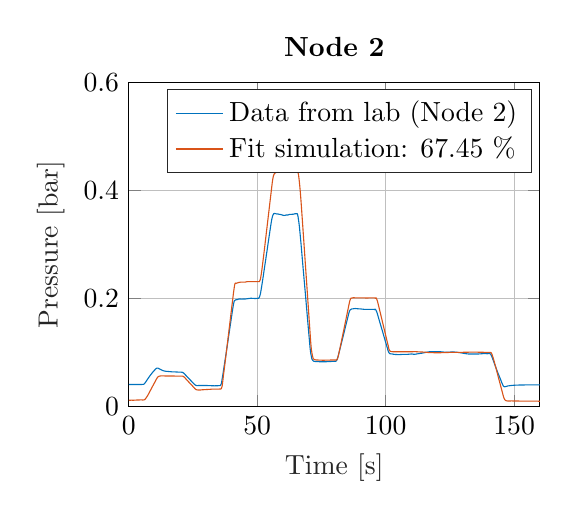
\begin{tikzpicture}

\begin{axis}[%
width=2.0556in,
height=1.62135in,
at={(0.766in,0.486in)},
scale only axis,
xmin=0,
xmax=160,
xlabel style={font=\color{white!15!black}},
xlabel={Time [s]},
ymin=0,
ymax=0.6,
ylabel style={font=\color{white!15!black}},
ylabel={Pressure [bar]},
axis background/.style={fill=white},
title style={font=\bfseries},
title={Node 2},
xmajorgrids,
ymajorgrids,
legend style={legend cell align=left, align=left, draw=white!15!black}
]
\addplot [color=mycolor1]
  table[row sep=crcr]{%
0.0500000000000114	0.0411290322580555\\
5.65000000000001	0.0412878787878697\\
5.84999999999999	0.0417094330400687\\
6.09999999999999	0.0426502932551216\\
6.40000000000001	0.0443242913000859\\
6.65000000000001	0.046010508308882\\
7.90000000000001	0.0548753665689219\\
8.59999999999999	0.0594330400782042\\
9.25	0.0633308895405662\\
9.69999999999999	0.0658235581622648\\
10.6	0.0703995601172949\\
10.8	0.0710471652003832\\
11	0.0714565004887504\\
11.15	0.0715237047898256\\
11.45	0.0712548875855248\\
11.85	0.0703384652981356\\
12.25	0.0693120723362597\\
12.65	0.0683162267839634\\
13.25	0.0669904692082071\\
13.9	0.0661107038123134\\
14.35	0.0657013685239463\\
16.95	0.0645772238514155\\
18.2	0.0644244868035173\\
19.7	0.064027370478982\\
20.3	0.0640945747800572\\
20.8	0.0637768817204289\\
21.05	0.0633247800586503\\
21.3	0.0625427663734115\\
21.65	0.0610703812316729\\
22.5	0.0567509775171118\\
23.15	0.0535801564027452\\
23.85	0.0500794232649184\\
24.75	0.0455156402736918\\
25.35	0.0424364613880641\\
25.75	0.0407380254154361\\
26.05	0.0398338220918788\\
26.3	0.0394061583577638\\
26.65	0.0391556695992108\\
27.55	0.0393206256109409\\
28.95	0.0393328445747727\\
30.45	0.039308406647109\\
30.8	0.0391984359726223\\
33.35	0.0387402248289277\\
35.55	0.0390884652981356\\
35.7	0.0395283479960824\\
35.85	0.0405608504398742\\
36	0.0421554252199314\\
36.05	0.0428274682306835\\
36.1	0.0438172043010638\\
36.2	0.0466092375366713\\
36.3	0.0496395405669716\\
36.55	0.0567509775171118\\
36.65	0.0597629521016643\\
36.8	0.0645039100684244\\
37.05	0.0724828934506263\\
37.35	0.0816898826979582\\
37.65	0.090780791788859\\
37.9	0.0984848484848442\\
38.15	0.106537145650037\\
38.35	0.112994868035202\\
38.7	0.124230205278593\\
38.95	0.132361925708693\\
39.25	0.141843841642242\\
39.45	0.148289345063546\\
40.25	0.173765884652994\\
40.65	0.186070381231673\\
40.75	0.188728005865102\\
40.9	0.192289833822088\\
41.05	0.195326246334304\\
41.1	0.195912756598233\\
41.2	0.1963220918866\\
41.35	0.196768084066463\\
41.55	0.197525659824038\\
41.7	0.19783724340175\\
42.3	0.198350439882688\\
42.85	0.199334066471152\\
42.95	0.199425708699891\\
43.4	0.199315738025405\\
44.15	0.199260752688161\\
44.3	0.199309628543489\\
45.35	0.199450146627555\\
45.65	0.199511241446714\\
45.8	0.19968230694036\\
47.5	0.20076368523948\\
48.05	0.200635386119245\\
48.35	0.200507086999011\\
49.1	0.200354349951112\\
49.45	0.200262707722374\\
49.7	0.200415444770272\\
49.8	0.200415444770272\\
50	0.200464320625599\\
50.55	0.200818670576723\\
50.75	0.201845063538599\\
50.95	0.203910068426183\\
51.05	0.205290811339182\\
51.15	0.207093108504381\\
51.35	0.211375855327475\\
51.45	0.214155669599222\\
51.75	0.222776148582597\\
52.4	0.242876344086028\\
52.6	0.249444037145651\\
52.8	0.255797898338216\\
52.95	0.260716031280538\\
53.1	0.265371456500475\\
53.2	0.268585043988253\\
53.35	0.273191593352891\\
53.4	0.274804496578696\\
53.55	0.280028103616814\\
53.8	0.287616080156397\\
53.95	0.292534213098719\\
54.1	0.297666177908098\\
54.25	0.302413245356803\\
54.35	0.305816226783975\\
54.7	0.31688049853372\\
54.95	0.324932795698913\\
55.15	0.331188905180824\\
55.25	0.334310850439891\\
55.45	0.340499755620726\\
55.55	0.343401759530792\\
55.75	0.34846041055718\\
55.9	0.351270772238507\\
56	0.352950879765388\\
56.15	0.354820381231661\\
56.4	0.357032013685227\\
56.55	0.357386363636351\\
56.65	0.357349706744856\\
56.75	0.357655180840652\\
57	0.357410801564015\\
57.2	0.357380254154435\\
57.5	0.356744868035179\\
57.7	0.356836510263918\\
57.85	0.356836510263918\\
57.95	0.356720430107515\\
58.05	0.356738758553263\\
58.45	0.356213343108493\\
58.5	0.356011730205267\\
58.95	0.355999511241436\\
59.05	0.355645161290312\\
59.75	0.354875366568905\\
59.95	0.354356060606051\\
60.05	0.354453812316706\\
60.25	0.354148338220909\\
60.4	0.353965053763432\\
60.6	0.354209433040069\\
60.8	0.354136119257078\\
61.25	0.354814271749774\\
61.5	0.35462487781038\\
61.65	0.354924242424261\\
61.75	0.354728739002951\\
61.95	0.35498533724342\\
62.05	0.355009775171084\\
62.1	0.354960899315756\\
62.35	0.355559628543517\\
62.7	0.355920087976557\\
62.95	0.356011730205296\\
63.3	0.356048387096791\\
63.7	0.356146138807446\\
63.75	0.356280547409597\\
63.95	0.356225562072353\\
64.4	0.356683773216048\\
64.5	0.356799853372451\\
64.65	0.357196969696986\\
64.75	0.357196969696986\\
64.85	0.357435239491707\\
64.95	0.357465786901287\\
65.05	0.357203079178902\\
65.2	0.35719086021507\\
65.35	0.357410801564043\\
65.55	0.357215298142734\\
65.7	0.355938416422305\\
65.75	0.355156402737066\\
65.85	0.352963098729248\\
65.9	0.351631231671576\\
66	0.348454301075293\\
66.1	0.345197947214075\\
66.2	0.342106549364615\\
66.25	0.34038978494624\\
66.35	0.336412512218971\\
66.45	0.331970918866091\\
66.6	0.324822825024455\\
66.75	0.317546432062585\\
67.05	0.301942815249276\\
67.15	0.296480938416437\\
67.3	0.288184261974607\\
67.5	0.277144428152496\\
67.65	0.268811094819171\\
67.75	0.263257575757592\\
67.85	0.257710166177901\\
68	0.249590664711633\\
68.1	0.244354838709683\\
68.3	0.233522727272742\\
68.65	0.21469941348974\\
68.9	0.200995845552313\\
69.6	0.162115102639291\\
69.7	0.156592130987292\\
70.1	0.13487292277614\\
70.25	0.126887829912022\\
70.35	0.121419843597266\\
70.45	0.115976295210174\\
70.5	0.113214809384147\\
70.55	0.110722140762448\\
70.7	0.104062805474086\\
70.75	0.102132209188653\\
70.85	0.0989736070381184\\
70.95	0.0962671065493623\\
71.15	0.0916666666666686\\
71.25	0.089510019550346\\
71.3	0.0887096774193594\\
71.4	0.087561094819165\\
71.55	0.0863453079178953\\
71.75	0.0851111925708778\\
71.9	0.0845246823069488\\
72.05	0.0842069892473205\\
72.4	0.0838648582600285\\
74.5	0.0832416911046039\\
75.7	0.083229472140772\\
76.65	0.0832600195503517\\
78.3	0.0837121212121303\\
79.05	0.0838770772238604\\
80.6	0.0842069892473205\\
80.75	0.084671309872931\\
80.9	0.0855266373411609\\
81.05	0.0868035190615899\\
81.15	0.0879032258064569\\
81.5	0.0936217008797655\\
81.7	0.0971285434995082\\
82.4	0.110282258064501\\
82.85	0.118749999999977\\
83.3	0.127437683284455\\
83.8	0.137237292277604\\
84.05	0.141990469208196\\
84.55	0.151686217008773\\
84.65	0.153696236559114\\
84.8	0.156573802541516\\
85.65	0.172770039100669\\
85.75	0.174468475073297\\
85.9	0.176472385141722\\
86	0.17761485826\\
86.15	0.179111681329402\\
86.7	0.180834555229694\\
87.15	0.181231671554229\\
87.3	0.181231671554229\\
87.7	0.181579912023437\\
88.2	0.181769305962831\\
89.65	0.181127810361659\\
89.75	0.181182795698902\\
90.2	0.180993401759508\\
90.6	0.18081011730203\\
90.85	0.180669599217964\\
91.05	0.180602394916889\\
91.2	0.180437438905159\\
91.85	0.180193059628522\\
92.35	0.180290811339177\\
92.55	0.180272482893429\\
92.9	0.180217497556185\\
93.65	0.180089198435951\\
94.95	0.180266373411513\\
95.4	0.180254154447681\\
95.55	0.180193059628522\\
95.7	0.179734848484827\\
95.75	0.179899804496557\\
95.8	0.180321358748756\\
95.85	0.180522971651982\\
95.95	0.18034579667642\\
96.05	0.179936461388053\\
96.2	0.178934506353841\\
96.45	0.176515151515133\\
96.55	0.175262707722368\\
96.75	0.172403470185714\\
96.9	0.169904692082099\\
97.7	0.15673264907133\\
97.95	0.152755376344061\\
98.85	0.138306451612891\\
99.1	0.13412145650048\\
99.4	0.129062805474092\\
100.5	0.11103372434016\\
100.6	0.109567448680338\\
100.7	0.108253910068413\\
100.75	0.107221407624621\\
100.8	0.105975073313772\\
100.85	0.104960899315728\\
100.95	0.103494623655905\\
101.05	0.102260508308888\\
101.25	0.100360459433034\\
101.4	0.0992974095796626\\
101.55	0.0985703812316672\\
101.75	0.0980388563049814\\
101.95	0.0979533235581584\\
102.55	0.0976417399804461\\
103.25	0.0969330400781985\\
103.5	0.0968719452590392\\
103.95	0.0967069892473091\\
105.15	0.0964198435972605\\
106.3	0.0968291788856561\\
108.45	0.0969758064516668\\
110.15	0.0976906158358304\\
110.75	0.0971896383187243\\
111.2	0.0970185728250783\\
111.65	0.0973423753666225\\
113.55	0.0988330889541089\\
113.85	0.0989369501466797\\
116.5	0.101392961876883\\
116.75	0.101557917888613\\
117.5	0.102040566959971\\
121.1	0.101900048875905\\
121.5	0.101722873900343\\
122.7	0.101154692082162\\
123.95	0.101148582600246\\
124.2	0.101148582600246\\
124.65	0.101191348973657\\
126.7	0.101282991202396\\
127.7	0.100885874877861\\
128.35	0.100336021505427\\
128.75	0.10009164222879\\
128.95	0.0999938905181352\\
129.25	0.0997861681329937\\
129.8	0.0993707233627106\\
131	0.0983443304008347\\
131.3	0.098148826979525\\
132.1	0.097727272727326\\
132.4	0.0975317693060163\\
132.65	0.0975745356794278\\
133.05	0.0976539589443348\\
134.4	0.0976600684262507\\
135.4	0.0975745356794278\\
136.45	0.0977394916911578\\
136.8	0.0979349951124675\\
137	0.0979411045943834\\
137.3	0.0980816226784498\\
137.6	0.0981732649071887\\
138.2	0.0983260019550869\\
139.55	0.0981366080156931\\
140.15	0.0984115347019099\\
140.5	0.0983870967742462\\
140.6	0.0981854838710206\\
140.75	0.097641739980503\\
140.95	0.0964076246334855\\
141.15	0.0946603128055301\\
141.35	0.0924731182795995\\
141.65	0.0886730205278923\\
141.95	0.0846652003910435\\
143.05	0.0704484359726507\\
143.6	0.063605816226783\\
144.2	0.0565371456500543\\
144.45	0.0536656891495397\\
144.9	0.0482465786901116\\
145.2	0.0445808895405548\\
145.6	0.0400659824046556\\
145.75	0.0388135386118904\\
145.95	0.0377077223851074\\
146.15	0.0371456500488421\\
146.35	0.0370234604105235\\
146.65	0.0372922776148243\\
147.6	0.0385386119256736\\
149.15	0.0395222385141381\\
151.2	0.0401087487780671\\
155.6	0.0404814271749387\\
160	0.0404386608015272\\
};
\addlegendentry{Data from lab (Node 2)}

\addplot [color=mycolor2]
  table[row sep=crcr]{%
0.0500000000000114	0.011956256109471\\
0.800000000000011	0.0120967741935374\\
1.05000000000001	0.0121639784946126\\
2	0.0120601173020418\\
2.55000000000001	0.0123594819159223\\
2.84999999999999	0.0123350439882586\\
3.09999999999999	0.0124389051808294\\
3.69999999999999	0.0125061094819046\\
4.80000000000001	0.0126710654936346\\
5	0.0126466275659709\\
5.55000000000001	0.0125183284457364\\
6	0.0127016129032143\\
6.19999999999999	0.0131659335288248\\
6.5	0.0145833333333201\\
7	0.0179802052786044\\
7.5	0.0217436461388161\\
7.69999999999999	0.0235581622678467\\
9.55000000000001	0.0401392961876752\\
9.94999999999999	0.0436094819159223\\
10.8	0.0512402248289447\\
11.1	0.0536168132942407\\
11.25	0.0545332355816299\\
11.45	0.0554496578690191\\
11.8	0.0564455034213154\\
12.05	0.0567693059628596\\
12.65	0.0572152981427223\\
13.45	0.057154203323563\\
14.25	0.0569159335288418\\
14.45	0.0568914956011781\\
14.65	0.0568853861192622\\
16.35	0.0569342619745896\\
17	0.0568487292277666\\
17.75	0.0568792766373463\\
18.1	0.0566959921798684\\
20	0.0567631964809436\\
20.55	0.0567204301075321\\
21	0.0566410068426251\\
21.2	0.0562622189638375\\
21.45	0.0554252199413554\\
21.65	0.0545576735092936\\
22	0.0528653470185816\\
22.35	0.0510141739980554\\
22.75	0.0489491691104718\\
23.1	0.0472385141740119\\
23.4	0.0456256109481785\\
24.4	0.0405364125122105\\
24.8	0.0385813782991136\\
25.65	0.0340603616813269\\
26.05	0.0322091886608007\\
26.25	0.031677663734115\\
26.55	0.0312438905180841\\
27.1	0.0309811827956992\\
27.95	0.0310422776148584\\
28.35	0.0313233137829911\\
31.9	0.0323252688172033\\
32.2	0.0324963343108493\\
32.8	0.0326979472140749\\
33.1	0.0326490713587475\\
34.55	0.0326368523949156\\
35.85	0.0328506842619731\\
35.95	0.0332661290322562\\
36.1	0.0342069892473091\\
36.15	0.0347446236559108\\
36.3	0.0371334310850386\\
36.35	0.0381109481915871\\
36.4	0.039558895405662\\
36.55	0.0448619257086875\\
36.6	0.046768084066457\\
36.85	0.0571847507331427\\
37.65	0.087554985337249\\
38.4	0.116495601173028\\
38.85	0.134420821114361\\
39.55	0.162328934506348\\
39.8	0.172275171065507\\
40.4	0.19602272727272\\
40.8	0.211265884652988\\
40.9	0.214937683284461\\
41.1	0.221676441837729\\
41.15	0.223118279569889\\
41.3	0.226649560117295\\
41.35	0.227663734115339\\
41.4	0.228201368523941\\
41.55	0.228824535679365\\
41.6	0.228885630498525\\
41.85	0.228366324535671\\
42.35	0.229319403714555\\
42.75	0.229887585532737\\
43.55	0.230620723362648\\
45.4	0.230730694037135\\
46.05	0.231396627565999\\
46.25	0.23145772238513\\
46.6	0.231561583577729\\
47.1	0.231579912023477\\
47.75	0.231641006842636\\
48.05	0.231653225806468\\
48.45	0.231555474095813\\
49.45	0.231653225806468\\
50.05	0.231500488758542\\
50.45	0.23150048875857\\
50.7	0.231573802541561\\
50.85	0.231702101661796\\
50.9	0.231928152492685\\
51.05	0.23321114369503\\
51.1	0.233858748778118\\
51.3	0.237396138807441\\
51.35	0.238526392961887\\
51.6	0.245692815249271\\
51.8	0.252559872922774\\
52.05	0.261638563049843\\
52.8	0.290689149560109\\
53.1	0.302883675464329\\
53.45	0.31704545454545\\
54.55	0.361528592375379\\
54.9	0.375873655913978\\
55.4	0.395931085043998\\
55.85	0.414002932551313\\
55.9	0.415811339198427\\
56.05	0.420717253176917\\
56.1	0.422134652981413\\
56.3	0.426625122189648\\
56.35	0.427517106549374\\
56.6	0.430467986314767\\
56.9	0.432123655913983\\
57.05	0.432746823069408\\
57.55	0.433773216031284\\
57.8	0.434011485826005\\
58.55	0.434145894428156\\
58.95	0.434133675464324\\
59.2	0.434158113391987\\
59.7	0.433987047898341\\
60.9	0.43428641251225\\
61.2	0.434188660801595\\
61.85	0.434054252199445\\
62.15	0.433925953079211\\
64.55	0.434090909090941\\
64.85	0.434231427175007\\
65.75	0.433877077223883\\
65.85	0.433565493646171\\
65.9	0.432942326490746\\
66.05	0.430321358748813\\
66.1	0.428897849462402\\
66.35	0.418908846529831\\
66.55	0.409762952101687\\
66.75	0.399499022482928\\
66.8	0.396627565982413\\
67.05	0.380828445747824\\
67.25	0.367656402737055\\
67.5	0.350635386119279\\
68.1	0.309347507331381\\
70.7	0.128427419354836\\
70.85	0.118334555229723\\
70.9	0.11547531769304\\
71.05	0.107740713587475\\
71.1	0.105687927663723\\
71.3	0.0996334310850386\\
71.4	0.0970369012707692\\
71.55	0.0935300586510266\\
71.75	0.089931573802545\\
71.8	0.0893450635386159\\
72	0.088147605083094\\
72.3	0.0873228250244438\\
72.55	0.0869562561094881\\
73.1	0.0865713587487846\\
73.65	0.086455278592382\\
74	0.0863758553274749\\
74.8	0.0862414467253245\\
75	0.0861498044965856\\
76.1	0.0861253665688935\\
76.5	0.0861742424242493\\
76.9	0.0862353372433802\\
77.45	0.0862597751710723\\
77.8	0.0862353372434086\\
78.05	0.0862475562072405\\
78.5	0.0864674975562139\\
78.8	0.0865469208211209\\
80.7	0.0864797165200457\\
80.85	0.0865652492668687\\
81.05	0.0873350439882756\\
81.15	0.0881598240469259\\
81.3	0.0897360703812353\\
81.5	0.0927724828934515\\
81.6	0.0948435972629511\\
81.95	0.102547653958936\\
82.3	0.110111192570855\\
83.5	0.137524437927681\\
83.8	0.144354838709688\\
85.8	0.190915200391032\\
85.95	0.193976050830912\\
86.1	0.196786412512239\\
86.3	0.199382942326508\\
86.5	0.200830889540583\\
86.6	0.201020283479977\\
86.95	0.20130131964811\\
87.3	0.201637341153514\\
87.75	0.201667888563094\\
88.05	0.201557917888607\\
89.65	0.201521260997112\\
90.05	0.201454056696036\\
92.75	0.201289100684306\\
94.55	0.201454056696036\\
94.8	0.201454056696036\\
95.1	0.201405180840709\\
95.75	0.201325757575802\\
95.85	0.201228005865119\\
96.05	0.200647605083105\\
96.25	0.201454056696008\\
96.3	0.201362414467269\\
96.5	0.199657869012725\\
96.8	0.195204056696014\\
96.95	0.192625855327492\\
97.55	0.180962854349985\\
99.65	0.139259530791833\\
99.85	0.135294477028395\\
100	0.132306940371507\\
100.85	0.115408113392022\\
101	0.113013196480978\\
101.05	0.112017350928681\\
101.25	0.107209188660846\\
101.3	0.106329423264953\\
101.5	0.104062805474143\\
101.8	0.102669843597312\\
102	0.102254398827029\\
102.3	0.10196725317698\\
103	0.101814516129082\\
103.5	0.101722873900343\\
105.2	0.101765640273754\\
107	0.101686217008847\\
107.15	0.101759530791838\\
107.85	0.10183284457483\\
108.2	0.101814516129082\\
110.2	0.101728983382259\\
110.8	0.101930596285484\\
111.35	0.101979472140812\\
111.95	0.101857282502493\\
112.25	0.101710654936511\\
112.6	0.101655669599268\\
113.45	0.101399071358799\\
115.2	0.101069159335339\\
115.4	0.100867546432113\\
115.65	0.100745356793794\\
117.1	0.100183284457529\\
117.6	0.100140518084118\\
118.05	0.10012218963837\\
118.35	0.100073313783042\\
118.6	0.100048875855379\\
118.95	0.0999694525904715\\
121.2	0.0998350439883211\\
121.7	0.100103861192622\\
122.35	0.100103861192622\\
122.65	0.100152737047949\\
123.1	0.100238269794772\\
123.35	0.100299364613932\\
123.55	0.100360459433091\\
124.25	0.100433773216082\\
125.2	0.100623167155476\\
126.1	0.100775904203374\\
126.3	0.100702590420383\\
127.05	0.100592619745896\\
127.75	0.100598729227812\\
128.65	0.100568181818232\\
128.85	0.100568181818232\\
129.1	0.100543743890569\\
129.45	0.100525415444821\\
130.2	0.100757575757626\\
130.55	0.100861436950197\\
131.1	0.100873655914029\\
132	0.100928641251272\\
134.15	0.101093597263002\\
134.8	0.101087487781086\\
136.1	0.100928641251272\\
136.55	0.10078201368529\\
136.85	0.100898093841693\\
137.45	0.100891984359777\\
137.7	0.100824780058701\\
138	0.100769794721458\\
138.45	0.100708699902299\\
139.95	0.100727028348047\\
140.6	0.100568181818232\\
140.8	0.100470430107578\\
141	0.100085532746874\\
141.2	0.09874144672537\\
141.45	0.096114369501521\\
141.65	0.0933162267839975\\
142	0.0877199413490075\\
142.15	0.0852333822092248\\
142.45	0.0800586510264338\\
142.8	0.0739186217008978\\
143.5	0.0612658846529825\\
143.85	0.0547226295210237\\
145.05	0.0331744868035173\\
145.5	0.025109970674464\\
145.75	0.0206072825024251\\
146	0.0165933528836604\\
146.2	0.0143450635385989\\
146.45	0.0125366568914842\\
146.65	0.0116752199413384\\
147.05	0.0109237536656792\\
147.3	0.0107832355816129\\
147.7	0.0105816226783872\\
148.1	0.0106427174975465\\
148.9	0.0107771260996969\\
150.95	0.0106121700879669\\
151.55	0.0106304985337147\\
152	0.0105266373411439\\
152.6	0.0104655425219846\\
152.9	0.0104716520039005\\
154.35	0.0104594330400687\\
159.15	0.0103066959921705\\
159.7	0.0102333822091794\\
159.95	0.0102761485825908\\
160	0.010263929618759\\
};
\addlegendentry{Fit simulation: 67.45 \%}

\end{axis}
\end{tikzpicture}%
\caption{Step response of one pump PI system.}
\label{fig:Tikz_PI_PUMP_GAIN}
\end{figure}

\begin{figure}[H]
\centering
% This file was created by matlab2tikz.
%
%The latest updates can be retrieved from
%  http://www.mathworks.com/matlabcentral/fileexchange/22022-matlab2tikz-matlab2tikz
%where you can also make suggestions and rate matlab2tikz.
%
\definecolor{mycolor1}{rgb}{0.00000,0.44700,0.74100}%
\definecolor{mycolor2}{rgb}{0.85000,0.32500,0.09800}%
%
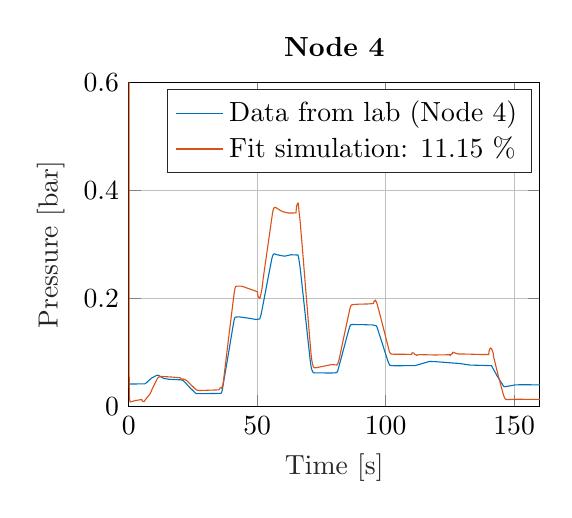
\begin{tikzpicture}

\begin{axis}[%
width=2.0556in,
height=1.62135in,
at={(0.766in,0.486in)},
scale only axis,
xmin=0,
xmax=160,
xlabel style={font=\color{white!15!black}},
xlabel={Time [s]},
ymin=0,
ymax=0.6,
ylabel style={font=\color{white!15!black}},
ylabel={Pressure [bar]},
axis background/.style={fill=white},
title style={font=\bfseries},
title={Node 4},
xmajorgrids,
ymajorgrids,
legend style={legend cell align=left, align=left, draw=white!15!black}
]
\addplot [color=mycolor1]
  table[row sep=crcr]{%
0.0500000000000114	0.0420454545454447\\
6.30000000000001	0.0423326001954933\\
7.05000000000001	0.0451185239491565\\
8.94999999999999	0.0532807917888647\\
10.85	0.0579545454545496\\
11.5	0.0583088954056734\\
12.4	0.0557612414467314\\
13.65	0.0524132453568029\\
15.65	0.0508553274682413\\
20	0.0498533724340291\\
21.1	0.0488636363636488\\
21.85	0.0453812316715414\\
24.15	0.0335838220918845\\
26.2	0.0243890518084129\\
27.2	0.024382942326497\\
30.1	0.0243340664711695\\
35.9	0.0247372922776208\\
36.15	0.0263990713587532\\
36.4	0.0308651026392965\\
36.7	0.0390334799608922\\
37.3	0.0559567448680411\\
38.25	0.0824474584555333\\
40.55	0.147996089931581\\
41.05	0.160764907135871\\
41.25	0.164161779081127\\
41.5	0.165860215053755\\
42.85	0.16642228739002\\
44	0.165603616813286\\
47.35	0.163453079178879\\
48.6	0.16220674486803\\
49.85	0.161455278592371\\
50.95	0.16250610948191\\
51.25	0.165786901270764\\
51.55	0.171407624633417\\
52.2	0.187096774193549\\
54.4	0.242253176930603\\
55.65	0.272763929618748\\
56	0.279142228739005\\
56.3	0.282044232649071\\
56.65	0.283058406647115\\
57.35	0.281738758553274\\
58.2	0.280791788856305\\
59.7	0.279356060606062\\
60.65	0.278586265884655\\
63.2	0.281256109481916\\
65.85	0.280712365591398\\
66.05	0.277535434995116\\
66.3	0.271065493646148\\
66.65	0.25932917888565\\
67	0.245521749755625\\
67.55	0.221169354838736\\
68.5	0.179313294232657\\
69.35	0.142088220918879\\
70.35	0.0980877321603089\\
70.75	0.0814760508309007\\
70.95	0.0748961388074463\\
71.2	0.06932429130012\\
71.6	0.0646994134897625\\
71.95	0.0629948680352186\\
72.6	0.0626466275660107\\
77.75	0.0625122189638603\\
80.1	0.0625610948191877\\
80.95	0.0633247800586787\\
81.25	0.0654081133920101\\
81.6	0.0706378299120445\\
85.55	0.140774682306954\\
86.05	0.148759775171072\\
86.35	0.151374633431089\\
86.75	0.152119990224833\\
90.95	0.152046676441842\\
92.45	0.15167399804497\\
94.85	0.151441837732165\\
96.45	0.149529569892479\\
96.85	0.144330400782025\\
100.75	0.0863208699902316\\
101.5	0.0771749755620874\\
101.9	0.0764846041055876\\
103.55	0.075763685239508\\
109.45	0.0761485826002115\\
110.85	0.0761119257087159\\
111.6	0.0763257575757734\\
117	0.0838037634408693\\
119.2	0.0834799608993251\\
128.75	0.0800158846529939\\
132.85	0.0771016617790963\\
141.15	0.0760813782991363\\
141.7	0.0715909090909008\\
143.35	0.0571725317692824\\
144.75	0.0464992668621562\\
145.95	0.0376282991202004\\
146.4	0.0370295698924394\\
150.55	0.0404814271749387\\
153.5	0.0407930107526511\\
160	0.0404081133919476\\
};
\addlegendentry{Data from lab (Node 4)}

\addplot [color=mycolor2]
  table[row sep=crcr]{%
0.0500000000000114	2.87707747843922\\
0.0999999999999943	0.263649529930916\\
0.150000000000006	0.091497572129839\\
0.199999999999989	0.0452379667079299\\
0.25	0.0270880262064566\\
0.300000000000011	0.0185412293807019\\
0.349999999999994	0.0140836632764376\\
0.449999999999989	0.0102819838409403\\
0.599999999999994	0.00887711426236137\\
0.949999999999989	0.00930013155607412\\
2.34999999999999	0.0112239631609725\\
5.05000000000001	0.013433653955957\\
5.09999999999999	0.0134424671839497\\
5.19999999999999	0.0111297151408962\\
5.34999999999999	0.0102355679974835\\
6	0.00954448752295889\\
6.19999999999999	0.0112418704499078\\
8.19999999999999	0.023271589523489\\
8.80000000000001	0.0286274967850773\\
9.09999999999999	0.0324096773759379\\
11.15	0.0522211657988692\\
11.7	0.054890622736707\\
12.45	0.0560480615677363\\
13.95	0.0557795314013845\\
17.1	0.0548710256818765\\
20.15	0.0535140742142346\\
20.3	0.0521367798952213\\
21	0.0504251019724791\\
21.15	0.0515529413933393\\
21.55	0.0509708142774059\\
22.15	0.0496145054118244\\
22.65	0.0481604085518086\\
25.75	0.03350308746991\\
26.55	0.0306900021199112\\
27.5	0.0300220042901742\\
35.15	0.0312370872850636\\
35.55	0.0346447653953135\\
36	0.0359709543546671\\
36.2	0.0343526919276087\\
36.4	0.0354150288764004\\
36.6	0.0393870322603789\\
36.9	0.0486491980218489\\
37.7	0.0807418994431259\\
39.35	0.145208979577745\\
40.85	0.203209260863787\\
41.2	0.215072864899298\\
41.4	0.219886719561259\\
41.6	0.222195828975231\\
42.05	0.223177353909193\\
43.95	0.223162435944886\\
49.2	0.214430116231568\\
50.1	0.212652391337087\\
50.2	0.207859035942363\\
50.35	0.204532060803757\\
50.7	0.201436698920077\\
51	0.200449526224219\\
51.2	0.204128613945102\\
51.55	0.210506040430971\\
51.85	0.218167021782193\\
51.95	0.221886148357299\\
52.2	0.232266345540467\\
52.65	0.247871749224061\\
55.95	0.357823426835353\\
56.2	0.363729532658709\\
56.45	0.367254685052302\\
56.75	0.368824316062984\\
57.25	0.368677163402594\\
59.15	0.362884355717227\\
60.45	0.36020757408545\\
62.3	0.35841655841017\\
64.4	0.358611294085165\\
65.1	0.358715339183959\\
65.2	0.365165147155153\\
65.3	0.369306201761333\\
65.45	0.372855816858817\\
65.7	0.375942021659711\\
65.95	0.376911120451553\\
66	0.376632194530913\\
66.1	0.369981507467259\\
66.3	0.360897239604213\\
66.6	0.348484218528966\\
66.85	0.336149664653448\\
66.9	0.333358263791837\\
66.95	0.329269423869931\\
67.5	0.298883501771229\\
68.65	0.2308523030392\\
70.55	0.120333832531969\\
70.95	0.0982216638363695\\
71.15	0.0896887479705697\\
71.4	0.082148559540542\\
71.65	0.0768124553414111\\
71.9	0.073783572971422\\
72.25	0.0722155977798877\\
72.9	0.0721769772812024\\
79	0.0780725836005445\\
80.75	0.0773534274079282\\
81.05	0.0773402569705297\\
81.45	0.0806140649421536\\
81.7	0.0843877941200333\\
82.25	0.0955614297302816\\
83.15	0.116450206885418\\
86.15	0.183015793463539\\
86.45	0.186874462757174\\
86.7	0.18830934851934\\
87.5	0.189206914774161\\
89.75	0.189892827340742\\
92.8	0.190132467817989\\
95.2	0.190973964150743\\
95.3	0.192880996713171\\
95.4	0.194122251654989\\
95.55	0.195643091504195\\
95.7	0.195731384587219\\
95.85	0.196208979409136\\
96	0.195501470136151\\
96.05	0.196451577780408\\
96.45	0.193492297209048\\
96.9	0.1871522734954\\
97	0.18433550528394\\
97.95	0.167531215339494\\
100.1	0.127091141525028\\
101.45	0.102110747073567\\
101.75	0.0992938855214618\\
102.15	0.0976885336776547\\
103.15	0.0971679003995973\\
107	0.0970671298743184\\
109.05	0.0970188203601197\\
110.1	0.0970149416945674\\
110.2	0.0993749442153558\\
110.45	0.099827356300068\\
111	0.099435893707664\\
111.1	0.0977786455460432\\
111.45	0.0967550150519969\\
111.9	0.0960372622790544\\
112	0.0950871411506569\\
112.95	0.0964944054075261\\
119.1	0.0957679417689121\\
122.8	0.0960600547285253\\
125.1	0.0962949444237324\\
125.15	0.0950753944568703\\
126	0.0988538737977933\\
126.05	0.100443555811808\\
126.2	0.100872389476535\\
128	0.0977182521800444\\
132	0.0974101265185539\\
136.5	0.0967629955093514\\
140.1	0.0966572788670419\\
140.2	0.101356910842213\\
140.35	0.104924403215335\\
140.55	0.107283259195469\\
140.85	0.108563394216532\\
141.25	0.107211680299059\\
141.8	0.10009203285955\\
141.9	0.0982443519762342\\
141.95	0.0947577381906228\\
142.1	0.0908425116551541\\
143.65	0.0605115003986896\\
145.75	0.0233570142181918\\
146.2	0.0170353357065665\\
146.6	0.0142565079273993\\
147.15	0.0132486303558892\\
150.4	0.0137732874013636\\
151.65	0.0138461249967463\\
157.75	0.013611905149304\\
159.3	0.0135764475834321\\
160	0.0135845159283861\\
};
\addlegendentry{Fit simulation: 11.15 \%}

\end{axis}
\end{tikzpicture}%
\caption{Step response of one pump PI system.}
\label{fig:Tikz_PI_PUMP_GAIN}
\end{figure}

\begin{figure}[H]
\centering
% This file was created by matlab2tikz.
%
%The latest updates can be retrieved from
%  http://www.mathworks.com/matlabcentral/fileexchange/22022-matlab2tikz-matlab2tikz
%where you can also make suggestions and rate matlab2tikz.
%
\definecolor{mycolor1}{rgb}{0.00000,0.44700,0.74100}%
\definecolor{mycolor2}{rgb}{0.85000,0.32500,0.09800}%
%
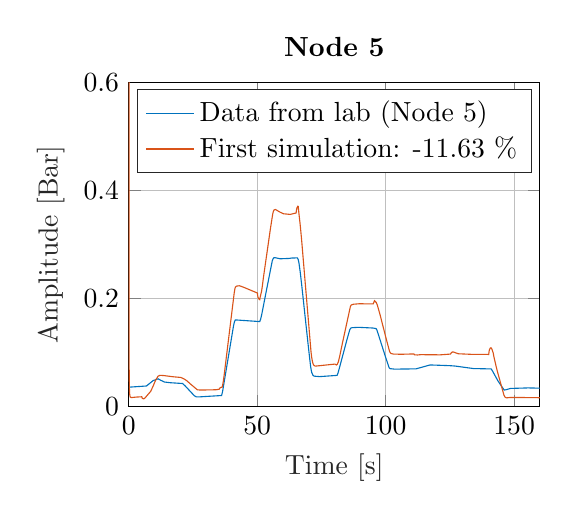
\begin{tikzpicture}

\begin{axis}[%
width=2.0556in,
height=1.62135in,
at={(0.766in,0.486in)},
scale only axis,
xmin=0,
xmax=160,
xlabel style={font=\color{white!15!black}},
xlabel={Time [s]},
ymin=0,
ymax=0.6,
ylabel style={font=\color{white!15!black}},
ylabel={Amplitude [Bar]},
axis background/.style={fill=white},
title style={font=\bfseries},
title={Node 5},
xmajorgrids,
ymajorgrids,
legend style={legend cell align=left, align=left, draw=white!15!black}
]
\addplot [color=mycolor1]
  table[row sep=crcr]{%
0.0500000000000114	0.0362231182795654\\
6.90000000000001	0.0383980938416357\\
9.5	0.048332111436963\\
11.45	0.0517106549364712\\
12.45	0.0490347018572947\\
13.95	0.045705034213114\\
16.2	0.0444525904203203\\
20.95	0.0430229716519932\\
21.9	0.0389112903225737\\
25.55	0.0203445747800686\\
26.3	0.0182612414467371\\
27.75	0.0183467741935601\\
36.15	0.0207905669599313\\
36.5	0.0273826979472176\\
36.95	0.0402614858259938\\
40.8	0.149822825024444\\
41.15	0.157325268817203\\
41.5	0.160703812316711\\
41.95	0.160551075268813\\
51	0.157594086021504\\
51.35	0.162133431085039\\
51.8	0.171425953079165\\
53.3	0.208088954056706\\
55.85	0.269550342130998\\
56.15	0.273466520039108\\
56.55	0.275898093841647\\
57.1	0.275696480938421\\
58.95	0.273796432062568\\
62.35	0.274450146627572\\
63.5	0.275207722385147\\
64.5	0.275287145650054\\
65.65	0.275549853372439\\
65.95	0.272617302052794\\
66.25	0.26617179863149\\
66.75	0.249236314760509\\
67.3	0.226380742912994\\
70	0.107441348973623\\
70.75	0.0760752688172204\\
71	0.0684567448680582\\
71.25	0.0630620723362938\\
71.7	0.0582783479961222\\
72.2	0.0565860215054101\\
74.3	0.0557612414467599\\
81.1	0.0580461876833169\\
81.45	0.0622922776148869\\
82.1	0.0735276148582784\\
85.1	0.1270711143695\\
86.05	0.142803030303043\\
86.4	0.145423998044976\\
86.85	0.146267106549374\\
89.4	0.146969696969705\\
95.05	0.145680596285445\\
96.3	0.144544232649082\\
96.6	0.141935483870981\\
97.15	0.13389540566962\\
98.2	0.11818792766374\\
99.9	0.0928091397849471\\
101.35	0.0722568426197654\\
101.7	0.07050953079181\\
103.45	0.0696236559140004\\
111.8	0.0700940860215269\\
117.3	0.0773582600195653\\
124.9	0.0760447214076407\\
127	0.0753299120234772\\
134.2	0.0706561583577923\\
141.05	0.0700085532747039\\
141.6	0.0659946236559108\\
143.6	0.0486620234603947\\
146.1	0.0309445259041752\\
146.65	0.0312561094818875\\
148.6	0.0338648582599888\\
155.4	0.034860703812285\\
160	0.0343780547409267\\
};
\addlegendentry{Data from lab (Node 5)}

\addplot [color=mycolor2]
  table[row sep=crcr]{%
0.0500000000000114	3.82183922500244\\
0.0999999999999943	0.276676402994013\\
0.150000000000006	0.104787143988091\\
0.199999999999989	0.058047327977107\\
0.25	0.0392739630695189\\
0.300000000000011	0.0301208295873039\\
0.349999999999994	0.0251240538277386\\
0.449999999999989	0.0203770596337165\\
0.599999999999994	0.0179389039132332\\
0.949999999999989	0.0169619099793294\\
3.05000000000001	0.0179374080923651\\
5.09999999999999	0.0184621098745197\\
5.25	0.0159305204320503\\
5.69999999999999	0.0146649483818919\\
6.15000000000001	0.0152535402844194\\
8.59999999999999	0.0287911715316511\\
8.90000000000001	0.0321648665274097\\
9.55000000000001	0.0385060699697135\\
9.84999999999999	0.042323981862495\\
10.6	0.0503512604374805\\
11.45	0.0566295759956859\\
12.2	0.0581741525921302\\
13.65	0.05770182671111\\
17.15	0.0555570925772599\\
20.25	0.0542007435054188\\
21.15	0.0523737843410004\\
21.65	0.0511605016012311\\
22.6	0.0482093092953733\\
23.9	0.0426300364363215\\
26.75	0.0312140244468253\\
28.4	0.0309302196525607\\
33.95	0.0314541836244757\\
35.2	0.0324100064932509\\
35.6	0.0354006006227507\\
36.1	0.0360059363650294\\
36.3	0.0360742786970434\\
36.5	0.0386718284306653\\
36.8	0.046620210441489\\
37.1	0.0568320834229326\\
39	0.130719208218039\\
41.05	0.210206810432112\\
41.35	0.218632839941733\\
41.55	0.221553614569586\\
42	0.223300955944495\\
43.1	0.223904289606963\\
44.75	0.22104479956576\\
50.1	0.210418045125692\\
50.15	0.207095173779123\\
50.3	0.202936967032429\\
50.55	0.199940496547896\\
51	0.198201901639948\\
51.1	0.201538617251771\\
51.7	0.213532798981959\\
52	0.223029857561016\\
52.4	0.23807647060994\\
55.15	0.329507295992244\\
56.05	0.356813537438256\\
56.3	0.361569506302374\\
56.6	0.364314597187757\\
57.1	0.365073998870457\\
58.7	0.360542193845902\\
60.2	0.3571097048914\\
62.85	0.355915890157974\\
65.15	0.358546682281343\\
65.3	0.364439772109307\\
65.5	0.368299401344984\\
65.85	0.371099590162146\\
66	0.370395279817558\\
66.1	0.364113729070937\\
66.4	0.351094274191809\\
66.7	0.33840533733553\\
67.25	0.311223095666378\\
68	0.2685693271319\\
70.95	0.101652339886613\\
71.2	0.0917362723325823\\
71.5	0.0837014510512688\\
71.75	0.0792922193554091\\
72.05	0.0766957944490798\\
72.65	0.0751795555712818\\
73.95	0.0758188348552551\\
80.2	0.0789109885612049\\
80.85	0.0772817342101177\\
81.15	0.0785132862552018\\
81.6	0.0832891132211842\\
82.1	0.0930976315280816\\
83.2	0.118307581623526\\
86.25	0.184965821104555\\
86.6	0.188238273968608\\
87.4	0.189675461069754\\
89.7	0.190575698096353\\
95.15	0.190293426523255\\
95.65	0.196145195233981\\
96.35	0.192866479447616\\
96.8	0.187435559497487\\
97.8	0.170638090421448\\
100.15	0.126815085328701\\
101.55	0.101855973052466\\
102.05	0.0986494907950259\\
102.95	0.0975011809577779\\
106	0.0970896506505881\\
111	0.0977346187480066\\
111.2	0.096188708580371\\
112.35	0.0957962707120714\\
113.65	0.0963792915596287\\
121.25	0.0960733535974612\\
125.25	0.0974644565331459\\
125.6	0.10039177989492\\
126.2	0.101615502098184\\
128.25	0.0980372625614052\\
133.9	0.0968803205231552\\
140.1	0.0967770681942\\
140.25	0.102504900463828\\
140.45	0.1063939257063\\
140.75	0.108678388725252\\
141	0.109048430497722\\
141.35	0.106768661344688\\
141.9	0.0990312575410144\\
142	0.0953019307828811\\
142.35	0.0878789654078673\\
142.95	0.0755363504925128\\
143.6	0.0632706925558182\\
146.05	0.0212299687878215\\
146.5	0.0175800342550474\\
147.05	0.016427594115811\\
148.2	0.017040462102841\\
150.2	0.017224401374051\\
160	0.0167107640661754\\
};
\addlegendentry{First simulation: -11.63 \%}

\end{axis}
\end{tikzpicture}%
\caption{Step response of one pump PI system.}
\label{fig:Tikz_PI_PUMP_GAIN}
\end{figure}

\begin{figure}[H]
\centering
% This file was created by matlab2tikz.
%
%The latest updates can be retrieved from
%  http://www.mathworks.com/matlabcentral/fileexchange/22022-matlab2tikz-matlab2tikz
%where you can also make suggestions and rate matlab2tikz.
%
\definecolor{mycolor1}{rgb}{0.00000,0.44700,0.74100}%
\definecolor{mycolor2}{rgb}{0.85000,0.32500,0.09800}%
%
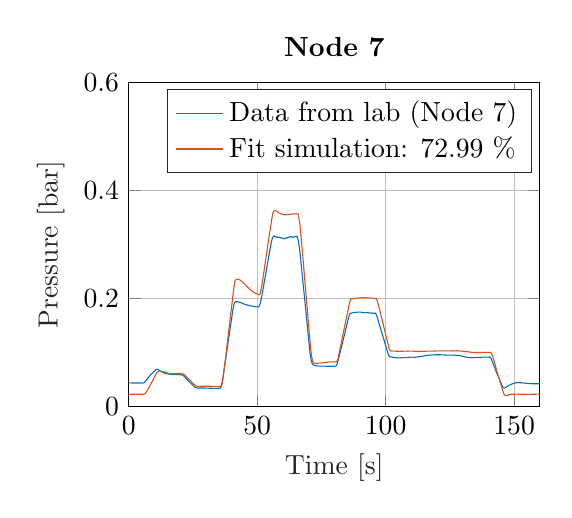
\begin{tikzpicture}

\begin{axis}[%
width=2.0556in,
height=1.62135in,
at={(0.766in,0.486in)},
scale only axis,
xmin=0,
xmax=160,
xlabel style={font=\color{white!15!black}},
xlabel={Time [s]},
ymin=0,
ymax=0.6,
ylabel style={font=\color{white!15!black}},
ylabel={Pressure [bar]},
axis background/.style={fill=white},
title style={font=\bfseries},
title={Node 7},
xmajorgrids,
ymajorgrids,
legend style={legend cell align=left, align=left, draw=white!15!black}
]
\addplot [color=mycolor1]
  table[row sep=crcr]{%
0.0500000000000114	0.0440493646138691\\
0.75	0.0440799120234487\\
2.65000000000001	0.0439821603127939\\
3.19999999999999	0.043969941348962\\
5.09999999999999	0.0438294232648957\\
5.44999999999999	0.0438294232648957\\
5.75	0.0440860215053647\\
5.94999999999999	0.0445075757575637\\
6.15000000000001	0.0452407135874751\\
6.40000000000001	0.0464687194525766\\
6.69999999999999	0.0482893450635515\\
8	0.0562500000000057\\
8.69999999999999	0.0600562072336288\\
9.30000000000001	0.0629337732160309\\
10.55	0.0683101173020475\\
10.8	0.0690676930596226\\
11	0.0693609481915871\\
11.15	0.0693242913000915\\
11.35	0.0690432551319589\\
11.6	0.0683467741935431\\
12.2	0.0663795210166143\\
12.45	0.0655730694037118\\
13.7	0.0625\\
14.5	0.0613758553274693\\
16.15	0.0599034701857306\\
17.2	0.0596529814271776\\
17.55	0.0596407624633457\\
18.7	0.0596346529814298\\
19.05	0.0594758064516157\\
19.55	0.0594330400782042\\
20.15	0.0592253176930626\\
20.4	0.0591825513196511\\
20.7	0.0589626099706777\\
20.95	0.0584799608993194\\
21.2	0.0577590420332399\\
21.6	0.0561461388074349\\
22.4	0.0522727272727366\\
22.65	0.0510263929618873\\
23.35	0.047489002932565\\
23.95	0.0446297653958823\\
25.55	0.0369501466275608\\
25.8	0.0359665200390964\\
26	0.0354777614858222\\
26.35	0.0349034701857249\\
26.65	0.0347690615835745\\
27.55	0.0347996089931542\\
28.05	0.0347751710654904\\
29.25	0.03464076246334\\
29.7	0.0345674486803489\\
30.1	0.0345185728250215\\
31.05	0.0343719452590392\\
31.7	0.0341947702834773\\
34.05	0.034048142717495\\
34.8	0.0341825513196454\\
35.5	0.0342864125122162\\
35.6	0.0344452590420303\\
35.7	0.0349156891495568\\
35.8	0.0355510752688133\\
35.9	0.0364736070381184\\
36	0.0376405180840607\\
36.05	0.0384775171065428\\
36.15	0.0407074780058565\\
36.45	0.0479411045943436\\
36.55	0.0507636852395024\\
36.65	0.0537573313783071\\
36.9	0.0618096285435001\\
37.15	0.0698069403714499\\
37.4	0.0775537634408749\\
38.1	0.100140518084061\\
38.3	0.106702101661767\\
38.45	0.111644672531781\\
38.7	0.119806940371461\\
38.95	0.127779814271747\\
39.65	0.150336021505382\\
39.85	0.156830400782013\\
40.2	0.168053519061573\\
40.4	0.174535679374401\\
40.6	0.180535190615842\\
40.7	0.18322336265885\\
40.85	0.186986803519062\\
40.95	0.189051808406646\\
41	0.189980449657867\\
41.05	0.19069525904203\\
41.15	0.191623900293251\\
41.45	0.194018817204295\\
41.55	0.194348729227755\\
41.7	0.194397605083083\\
41.9	0.194305962854344\\
42.05	0.194244868035184\\
42.45	0.194379276637335\\
43.1	0.193609481915928\\
43.3	0.19323069403714\\
43.4	0.193035190615831\\
43.7	0.192173753665685\\
43.85	0.192082111436946\\
44.15	0.191544477028344\\
44.4	0.191012952101659\\
44.8	0.190255376344084\\
44.9	0.189962121212119\\
45.15	0.189632209188659\\
45.35	0.188996823069402\\
45.5	0.188966275659823\\
45.65	0.188886852394916\\
45.8	0.188581378299119\\
45.9	0.18835532746823\\
46.25	0.188312561094818\\
46.35	0.18799486803519\\
46.65	0.187518328445748\\
46.85	0.187445014662757\\
47.35	0.186821847507332\\
47.5	0.186687438905182\\
47.95	0.186217008797655\\
48.2	0.186052052785925\\
48.5	0.185410557184753\\
48.75	0.185386119257089\\
48.9	0.185227272727275\\
49.1	0.185184506353863\\
49.25	0.185153958944284\\
49.5	0.185043988269797\\
50.1	0.184671309872925\\
50.5	0.184732404692085\\
50.6	0.184946236559142\\
50.75	0.185807673509288\\
50.85	0.186766862170089\\
51.1	0.189778836754641\\
51.2	0.191275659824043\\
51.25	0.192253176930592\\
51.35	0.19447702834799\\
51.45	0.19665200391006\\
51.7	0.202376588465313\\
51.8	0.204967008797666\\
51.9	0.207759042033246\\
52.1	0.212713831867063\\
52.3	0.218230694037146\\
52.75	0.230577956989237\\
52.95	0.235606060606074\\
53.1	0.239503910068436\\
53.2	0.24200268817205\\
53.45	0.249028592375367\\
53.9	0.261601906158347\\
54.05	0.265554740957981\\
54.25	0.271053274682316\\
54.45	0.276441837732165\\
54.9	0.288892961876826\\
55.05	0.293071847507321\\
55.25	0.298075513196466\\
55.35	0.300635386119268\\
55.6	0.306414956011736\\
55.85	0.310746578690129\\
55.95	0.311980694037146\\
56.05	0.31302541544477\\
56.2	0.314192326490712\\
56.3	0.314516129032256\\
56.4	0.315108748778101\\
56.55	0.315829667644181\\
56.65	0.316165689149557\\
56.7	0.316196236559136\\
56.75	0.316043499511238\\
56.9	0.315224828934504\\
57	0.315212609970672\\
57.05	0.315243157380252\\
57.3	0.314595552297163\\
57.5	0.314070136852393\\
57.6	0.313954056695991\\
57.65	0.313721896383186\\
57.7	0.31365469208211\\
57.8	0.313825757575756\\
57.9	0.313874633431084\\
58.05	0.31352028347996\\
58.2	0.313996823069402\\
58.55	0.313477517106548\\
58.7	0.313288123167155\\
58.9	0.313141495601172\\
59.2	0.312707722385142\\
59.3	0.312866568914956\\
59.95	0.311418621700881\\
60.05	0.311241446725319\\
60.15	0.311394183773217\\
60.45	0.310685483870969\\
60.6	0.311162023460412\\
60.7	0.31167521994135\\
60.9	0.311540811339199\\
61.15	0.31213954056696\\
61.3	0.312640518084066\\
61.5	0.312316715542522\\
61.7	0.312090664711633\\
61.85	0.312805474095796\\
61.95	0.313172043010752\\
62.05	0.313165933528836\\
62.15	0.313367546432062\\
62.25	0.313477517106548\\
62.55	0.314222873900292\\
62.8	0.314516129032256\\
62.9	0.314668866080154\\
62.95	0.31487047898338\\
63.05	0.31470552297165\\
63.25	0.314064027370478\\
63.6	0.314057917888562\\
63.75	0.313673020527858\\
63.95	0.313758553274681\\
64.2	0.31421065493646\\
64.35	0.314155669599216\\
64.5	0.314412267839685\\
64.7	0.315163734115345\\
64.75	0.315304252199411\\
65	0.31473607038123\\
65.15	0.314412267839685\\
65.25	0.314797165200389\\
65.35	0.315298142717495\\
65.4	0.315347018572822\\
65.55	0.314809384164221\\
65.6	0.314235092864124\\
65.7	0.312768817204301\\
65.75	0.31217008797654\\
65.8	0.311418621700881\\
65.9	0.309433040078204\\
66	0.307368035190621\\
66.05	0.306482160312811\\
66.1	0.305419110459439\\
66.15	0.303946725317701\\
66.3	0.298478739002945\\
66.65	0.28513563049853\\
66.7	0.283058406647115\\
66.95	0.271505376344095\\
67.1	0.264705522971639\\
67.2	0.260092864125113\\
67.35	0.252755376344084\\
67.45	0.247702834799611\\
67.6	0.240505865102648\\
68.05	0.219086021505376\\
68.35	0.20532135874879\\
68.95	0.17719330400783\\
69.35	0.157612414467252\\
69.5	0.150421554252205\\
69.7	0.140463098729242\\
69.9	0.131054496578685\\
70	0.126429618768327\\
70.15	0.119556451612908\\
70.4	0.107685728250232\\
70.55	0.100928641251215\\
70.6	0.0989491691104547\\
70.75	0.0937683284457478\\
70.85	0.0908846529814298\\
71	0.0869440371456562\\
71.05	0.0854899804496654\\
71.1	0.0842069892473205\\
71.15	0.0832050342131083\\
71.25	0.0817693059628652\\
71.4	0.0803641251222018\\
71.65	0.0782807917888704\\
71.8	0.0776576246334457\\
72.05	0.0769000488758707\\
72.25	0.0765151515151672\\
72.45	0.0764296187683442\\
72.7	0.0761180351906319\\
72.9	0.0759103128054903\\
73.15	0.0758858748778266\\
73.75	0.0754704301075435\\
73.95	0.075262707722402\\
75.55	0.0751221896383356\\
76.1	0.0750488758553445\\
76.4	0.0750427663734285\\
77	0.0748228250244551\\
77.65	0.0748900293255303\\
77.9	0.0750366568915126\\
78.1	0.0749572336266056\\
78.3	0.0749572336266056\\
78.7	0.074835043988287\\
78.95	0.0750244379276808\\
80.1	0.0749022482893622\\
80.3	0.0748228250244551\\
80.6	0.0752749266862338\\
80.75	0.0759042033235744\\
81	0.0778409090909236\\
81.1	0.0788673020527995\\
81.15	0.0795149071358878\\
81.25	0.0813172043010866\\
81.95	0.0945381231671547\\
82.65	0.107844574780046\\
82.95	0.113489736070392\\
83.6	0.126264662756597\\
83.75	0.129227761485822\\
84.05	0.134793499511233\\
84.25	0.138746334310838\\
84.65	0.146761974584535\\
85.35	0.160752688172039\\
85.6	0.165438660801556\\
85.75	0.167870234604095\\
85.95	0.17047287390028\\
86.1	0.172030791788842\\
86.15	0.172391251221882\\
86.25	0.172672287390014\\
86.65	0.173380987292262\\
87.1	0.173912512218948\\
87.25	0.174040811339182\\
87.45	0.174248533724324\\
87.65	0.174334066471147\\
88.2	0.174725073313766\\
88.45	0.174773949169094\\
88.65	0.174859481915917\\
88.75	0.17474951124143\\
89.25	0.175158846529797\\
89.6	0.175042766373394\\
89.9	0.17521383186704\\
90.2	0.175091642228722\\
90.5	0.174963343108487\\
90.85	0.174608993157364\\
91.2	0.174266862170072\\
91.4	0.174004154447687\\
91.75	0.174236314760492\\
91.9	0.17408968719451\\
92.1	0.17408968719451\\
92.25	0.174211876832828\\
92.65	0.174144672531753\\
92.8	0.17408968719451\\
93.15	0.173949169110443\\
93.65	0.173655913978479\\
93.8	0.173710899315722\\
94.15	0.173497067448665\\
94.4	0.173478739002917\\
94.55	0.173380987292262\\
94.7	0.173216031280532\\
94.9	0.173032746823054\\
95.2	0.173099951124129\\
95.35	0.173112170087961\\
95.55	0.173112170087961\\
95.75	0.172696725317678\\
95.8	0.173148826979457\\
95.85	0.173411534701842\\
95.9	0.173484848484833\\
96	0.173002199413475\\
96.35	0.170570625610935\\
96.45	0.16945259042032\\
96.55	0.168084066471152\\
96.8	0.164235092864118\\
96.95	0.161895161290317\\
97.15	0.158528836754641\\
97.3	0.156017839687195\\
97.85	0.147360703812296\\
98	0.145002443792748\\
98.65	0.135025659824038\\
98.9	0.131042277614853\\
99.15	0.127034457478004\\
99.45	0.121945259042036\\
99.9	0.114870478983363\\
100.1	0.111583577712594\\
100.6	0.103500733137821\\
100.7	0.102352150537627\\
100.75	0.10138685239491\\
100.8	0.100134408602145\\
100.85	0.0990835777126051\\
100.9	0.0981915933528796\\
101	0.0970063538611896\\
101.3	0.0940738025415442\\
101.4	0.0933834310850443\\
101.55	0.0927236070381241\\
101.7	0.0924547898338233\\
102	0.0921309872922791\\
102.35	0.0920271260997083\\
102.75	0.0916849951124163\\
104	0.0907502443792794\\
104.55	0.0905486314760537\\
104.9	0.090438660801567\\
105.2	0.0904569892473148\\
105.55	0.0905486314760537\\
105.7	0.0906341642228767\\
108.3	0.0910862658846554\\
108.5	0.0911045943304032\\
108.65	0.0911351417399828\\
109.1	0.0914650537634429\\
109.3	0.0915139296187704\\
109.6	0.0917827468230712\\
109.8	0.0918316226783986\\
110.15	0.0918682795698942\\
111.3	0.091373411534704\\
111.7	0.0917827468230712\\
112.5	0.0922287390029339\\
112.8	0.0924425708699914\\
113.15	0.092735826001956\\
113.5	0.0928274682306949\\
113.7	0.0929618768328453\\
114.05	0.093157380254155\\
114.25	0.0934384164222877\\
115.6	0.0945320136852388\\
115.8	0.0948252688172033\\
116.3	0.0952590420332342\\
118.45	0.095906647116351\\
118.7	0.0960349462365855\\
119.05	0.0961143695014925\\
120.35	0.0962609970675032\\
120.75	0.0963282013685784\\
122.15	0.0959371945259591\\
122.55	0.0959188660802113\\
122.8	0.0958516617791361\\
122.95	0.0958638807429679\\
124.05	0.095436217008853\\
124.65	0.09551564027376\\
125.4	0.0954606549365167\\
125.95	0.0954545454546007\\
126.55	0.0954850928641804\\
127.3	0.095265151515207\\
127.85	0.0951735092864681\\
128.1	0.094923020527915\\
128.3	0.0949657869013265\\
128.6	0.0946419843597823\\
128.8	0.0945442326491275\\
128.95	0.0945686705767912\\
130.3	0.0928946725318269\\
130.6	0.0925708699902827\\
130.8	0.0923631476051412\\
131	0.0922715053764023\\
131.25	0.0919477028348581\\
131.4	0.0918377321603714\\
131.65	0.0916849951124732\\
132.5	0.0910801564027963\\
133.85	0.0909518572825618\\
134.1	0.0909762952102255\\
134.5	0.090933528836814\\
134.7	0.0909762952102255\\
134.9	0.0908907624634026\\
135.05	0.0908174486804114\\
136.05	0.0913245356794334\\
136.6	0.0912573313783582\\
137.2	0.091532258064575\\
137.55	0.0916911045943891\\
137.85	0.091703323558221\\
138.4	0.0917644183773803\\
138.55	0.091788856305044\\
138.7	0.0918316226784555\\
138.9	0.0917094330401369\\
139.9	0.0919660312806059\\
140.2	0.0920882209189244\\
140.45	0.0919293743891103\\
140.65	0.091446725317752\\
140.85	0.0903958944282124\\
141.1	0.0885569403715181\\
141.25	0.0871212121212466\\
141.45	0.0847812805474462\\
141.7	0.0816654447703229\\
142.25	0.0746151026393136\\
142.85	0.067027126099731\\
143.1	0.0639540566960193\\
143.35	0.0610520527859251\\
143.95	0.0543866080156477\\
144.25	0.051014173998027\\
144.65	0.0466703323558022\\
144.9	0.0437744379276523\\
145.5	0.0373411534701518\\
145.65	0.0361986803518732\\
145.8	0.0353372434017274\\
145.95	0.0347812805473779\\
146.1	0.034518572824993\\
146.3	0.0346590909090594\\
146.5	0.0350989736070062\\
148.2	0.0401576246333946\\
149.4	0.0425158846529428\\
150.6	0.0443059628543097\\
151.15	0.0445808895405264\\
152.1	0.0445503421309468\\
153.05	0.0442937438904778\\
155.2	0.0431207233626196\\
157	0.0426075268816817\\
159.35	0.0424670087976153\\
160	0.0425586510263543\\
};
\addlegendentry{Data from lab (Node 7)}

\addplot [color=mycolor2]
  table[row sep=crcr]{%
0.0500000000000114	0.0229472140762539\\
0.449999999999989	0.0229227761485902\\
1.15000000000001	0.0230388563049928\\
1.44999999999999	0.0230510752688247\\
1.94999999999999	0.0231121700879839\\
2.65000000000001	0.0230755131964884\\
3.84999999999999	0.0232465786901344\\
4.30000000000001	0.0231182795698999\\
6	0.0232404692082184\\
6.19999999999999	0.0237292277614927\\
6.40000000000001	0.0244745845552359\\
6.65000000000001	0.0259164222873949\\
7.05000000000001	0.0288062072336288\\
8.5	0.0409885141739892\\
8.94999999999999	0.0450146627565857\\
9.65000000000001	0.0514540566960022\\
10.7	0.0609359726295224\\
11	0.0632881231671547\\
11.2	0.0645405669599199\\
11.4	0.0654325513196454\\
11.6	0.0659152003910037\\
11.85	0.0661412512218931\\
12.35	0.0659396383186674\\
12.95	0.0655730694037118\\
13.75	0.0646444281524907\\
15.65	0.0617668621700886\\
16.1	0.0613453079178896\\
16.7	0.0609787390029339\\
18.85	0.0611009286412525\\
20.35	0.0610642717497569\\
20.85	0.0610398338220932\\
21.3	0.0603250244379296\\
21.65	0.0592008797653989\\
21.95	0.0579239980449699\\
22.45	0.0555779569892536\\
24.2	0.0471529814271605\\
24.45	0.0460410557184616\\
25.05	0.0433223362658737\\
25.3	0.0421126588465199\\
25.8	0.0397971652003832\\
26.1	0.0387280058650958\\
26.4	0.0381353861192508\\
26.75	0.0377321603127996\\
27	0.0377260508308837\\
27.65	0.0378360215053704\\
27.95	0.0379093352883615\\
30.05	0.0380193059628482\\
35.2	0.037524437927658\\
35.6	0.037530547409574\\
35.8	0.0375672043010695\\
36	0.0379154447702774\\
36.05	0.0382270283479897\\
36.2	0.0396810850439806\\
36.25	0.0404630987292194\\
36.45	0.0448497067448557\\
36.5	0.0462793255131828\\
36.8	0.0566043499511295\\
36.9	0.0599767839687217\\
37.05	0.0655180840664684\\
37.2	0.0711388074291222\\
37.75	0.0927847018572834\\
37.95	0.100775904203317\\
38.2	0.110929863147618\\
38.4	0.118884408602156\\
40.55	0.205431329423249\\
40.7	0.211455278592382\\
40.8	0.215444770283483\\
41	0.222947214076243\\
41.05	0.224621212121207\\
41.2	0.229099462365582\\
41.25	0.230296920821104\\
41.45	0.233657135874864\\
41.5	0.23415811339197\\
41.85	0.235581622678382\\
41.95	0.235978739002917\\
42.25	0.236162023460395\\
42.95	0.23534335288366\\
43.15	0.234738514173984\\
43.45	0.234060361681315\\
43.9	0.232484115347006\\
44.15	0.231341642228728\\
44.45	0.230058651026383\\
44.9	0.228018084066463\\
45.05	0.227339931573795\\
45.2	0.226710654936454\\
45.4	0.225733137829906\\
45.7	0.224272971651999\\
45.9	0.223148826979468\\
46.15	0.221963587487778\\
46.35	0.220894428152491\\
46.55	0.220075757575756\\
46.7	0.219477028347995\\
47.9	0.214467253176934\\
48.1	0.213660801564032\\
48.4	0.212518328445753\\
49.25	0.210166177908093\\
50.65	0.20738025415443\\
50.75	0.207343597262934\\
50.95	0.207642961876815\\
51.1	0.208913734115328\\
51.15	0.209384164222854\\
51.2	0.210117302052765\\
51.4	0.21397849462366\\
51.5	0.21634897360704\\
51.65	0.220155180840663\\
52	0.230333577712599\\
52.1	0.233321114369488\\
52.35	0.241342864125102\\
52.65	0.250702590420332\\
52.85	0.257313049853366\\
53.05	0.263850195503409\\
53.3	0.271975806451621\\
53.8	0.288147605083083\\
54.1	0.298081622678382\\
54.25	0.302840909090918\\
54.55	0.312273949169111\\
54.85	0.32184750733137\\
55.35	0.337255620723369\\
55.65	0.346505376344084\\
55.75	0.34948069403714\\
55.9	0.353580156402728\\
55.95	0.354814271749746\\
56.15	0.358913734115333\\
56.2	0.359707966764404\\
56.4	0.361705767350912\\
56.5	0.362188416422271\\
56.65	0.362732160312788\\
57	0.363123167155408\\
57.1	0.363013196480921\\
57.3	0.362365591397833\\
57.45	0.362182306940355\\
57.55	0.362072336265868\\
57.7	0.361485826001939\\
57.9	0.360697702834784\\
58.3	0.359494134897346\\
58.85	0.35797287390028\\
59.05	0.357380254154435\\
59.3	0.356958699902236\\
59.45	0.356598240469197\\
59.85	0.356048387096791\\
60.3	0.355663489736088\\
60.55	0.355596285435013\\
60.75	0.355419110459451\\
60.85	0.355419110459451\\
61.05	0.355694037145668\\
61.5	0.355541300097769\\
62.3	0.355669599218004\\
62.5	0.355749022482911\\
62.7	0.355852883675482\\
62.9	0.356188905180858\\
63.6	0.356647116324552\\
63.8	0.3566654447703\\
65.25	0.357123655913995\\
65.5	0.356952590420349\\
65.85	0.35699535679376\\
65.9	0.35650048875857\\
66.1	0.353030303030323\\
66.15	0.351838954056717\\
66.45	0.342833577712639\\
66.55	0.33984604105575\\
66.6	0.337933773216065\\
66.8	0.328512952101676\\
66.9	0.32357038123169\\
67.1	0.313330889540595\\
67.35	0.300085532746834\\
67.55	0.28922898338223\\
67.7	0.28105449657869\\
68.55	0.233198924731198\\
69.35	0.188966275659823\\
69.9	0.158577712609969\\
70.05	0.150226050830895\\
70.25	0.139076246334298\\
70.85	0.106286656891484\\
70.9	0.103995601173011\\
71.1	0.0962304496578668\\
71.15	0.0946419843597255\\
71.55	0.0847690615835859\\
71.6	0.0838954056696082\\
71.85	0.0818059628543324\\
72.1	0.0807978983382043\\
72.6	0.0799059139784788\\
73.1	0.0800158846529655\\
74	0.0806390518083901\\
74.8	0.0809567448680184\\
75.3	0.081243890518067\\
75.55	0.0812927663733944\\
76.35	0.081836510263912\\
76.8	0.0821358748777925\\
77.1	0.0823863636363455\\
77.35	0.0824718963831685\\
78	0.0828079178885446\\
78.75	0.0830828445747613\\
79.15	0.0829362170087791\\
79.35	0.0830034213098543\\
79.7	0.0831195014662569\\
79.85	0.0830889540566773\\
80.45	0.0831805962854162\\
80.8	0.0832050342130799\\
80.9	0.0835532746822878\\
81.1	0.0845002443792566\\
81.3	0.086711876832851\\
81.5	0.0898582600195539\\
81.55	0.0908846529814298\\
81.75	0.0958822091886589\\
82.15	0.104997556207223\\
82.55	0.114125122189648\\
82.8	0.119721407624638\\
82.95	0.123161045943306\\
83.35	0.13250244379276\\
85.85	0.190499755620749\\
86.1	0.195326246334332\\
86.25	0.197360703812336\\
86.35	0.198258797653978\\
86.5	0.199340175953097\\
86.55	0.199456256109499\\
86.75	0.199297409579685\\
87.4	0.199835043988287\\
87.95	0.200409335288384\\
88.35	0.200568181818198\\
88.7	0.200867546432079\\
88.95	0.201087487781052\\
89.4	0.201337976539605\\
90.2	0.201380742913017\\
90.5	0.201594574780074\\
91	0.201692326490729\\
91.3	0.201606793743906\\
91.65	0.201643450635402\\
91.85	0.201527370478999\\
92.3	0.201643450635402\\
92.6	0.201588465298158\\
92.85	0.20163123167157\\
93.1	0.201490713587503\\
93.55	0.20130131964811\\
94.1	0.201026392961893\\
94.25	0.201056940371473\\
94.55	0.200934750733154\\
94.95	0.201008064516145\\
95.8	0.200476539589459\\
95.95	0.200109970674504\\
96.05	0.200256598240486\\
96.2	0.20061094819161\\
96.25	0.200568181818198\\
96.45	0.199828934506371\\
96.5	0.199364613880761\\
96.9	0.193578934506377\\
97	0.191813294232674\\
98.2	0.168811094819176\\
98.65	0.160013440860212\\
98.95	0.154313294232651\\
99.3	0.147519550342139\\
99.45	0.144672531769288\\
99.65	0.140719696969683\\
100.6	0.122262952101636\\
101	0.114803274682288\\
101.2	0.110428885630483\\
101.3	0.108706011730192\\
101.45	0.106304985337232\\
101.5	0.105785679374378\\
101.75	0.104423264907126\\
101.95	0.103561827956952\\
102.3	0.103128054740921\\
102.65	0.103048631476014\\
102.95	0.102877565982368\\
103.15	0.102883675464284\\
103.65	0.102871456500452\\
103.95	0.10272482893447\\
104.6	0.102614858260011\\
105	0.102578201368516\\
105.55	0.102584310850432\\
106.9	0.10281036168135\\
107.05	0.10281036168135\\
108.35	0.102840909090958\\
108.55	0.102761485826051\\
109.25	0.10295698924736\\
109.65	0.102865347018621\\
109.9	0.102883675464369\\
110.2	0.102950879765444\\
111.9	0.102474340176002\\
112.55	0.102572091886657\\
112.75	0.102498778103666\\
113.5	0.102633186705816\\
114.2	0.102486559139834\\
114.75	0.102559872922825\\
114.95	0.102529325513245\\
115.3	0.102547653958993\\
115.9	0.102840909090958\\
116.45	0.102908113392033\\
116.8	0.102908113392033\\
117.95	0.102950879765444\\
118.2	0.102816471163294\\
120.4	0.103494623655962\\
121.6	0.103488514174046\\
121.85	0.10351295210171\\
122.2	0.103293010752736\\
122.35	0.103256353861241\\
122.65	0.103329667644232\\
122.85	0.103384652981475\\
123.95	0.103531280547458\\
124.75	0.10328690127082\\
125.45	0.103341886608064\\
125.8	0.103244134897409\\
126.15	0.103231915933577\\
127.6	0.103635141740028\\
127.8	0.103592375366617\\
129.8	0.102963098729276\\
130.05	0.102773704789882\\
130.6	0.102517106549413\\
131	0.102419354838759\\
131.35	0.102156647116374\\
131.7	0.102028347996139\\
132.1	0.101698435972679\\
132.45	0.101356304985387\\
133.35	0.100830889540617\\
133.7	0.100714809384215\\
133.95	0.100641495601224\\
134.35	0.100543743890569\\
134.95	0.100409335288418\\
135.15	0.100415444770334\\
135.45	0.100360459433091\\
135.95	0.100323802541595\\
137.2	0.10045210166183\\
137.35	0.10045210166183\\
137.6	0.100433773216082\\
137.9	0.100568181818232\\
138.3	0.100568181818232\\
138.5	0.100690371456551\\
139.5	0.100580400782064\\
139.75	0.100635386119308\\
140.05	0.100574291300148\\
140.4	0.100445992179914\\
140.8	0.100311583577763\\
140.95	0.0998900293255645\\
141.05	0.0994623655914495\\
141.3	0.0973607038123703\\
141.5	0.0950696480938689\\
141.8	0.0907991202346352\\
142	0.0876955034213438\\
142.4	0.0811094819159734\\
142.65	0.0768817204301229\\
143.35	0.0645833333333599\\
143.65	0.0597751710654961\\
144.05	0.0535373900293337\\
144.4	0.0481304985337374\\
145.85	0.0259469696969461\\
146.05	0.0235642717497342\\
146.3	0.0217680840664514\\
146.5	0.0209066471163055\\
146.7	0.0205828445747613\\
147	0.0206561583577525\\
147.7	0.021548142717478\\
148.1	0.0224951124144468\\
148.4	0.0229105571847299\\
149.05	0.0231060606060396\\
150.05	0.0231304985337033\\
150.65	0.0232771260996856\\
151.65	0.0232587976539378\\
152.2	0.0231977028347785\\
154.15	0.0230571847507122\\
154.5	0.023069403714544\\
155.4	0.0229288856304777\\
155.7	0.0229166666666458\\
156.1	0.0229655425219732\\
160	0.023411534701836\\
};
\addlegendentry{Fit simulation: 72.99 \%}

\end{axis}
\end{tikzpicture}%
\caption{Step response of one pump PI system.}
\label{fig:Tikz_PI_PUMP_GAIN}
\end{figure}

\begin{figure}[H]
\centering
% This file was created by matlab2tikz.
%
%The latest updates can be retrieved from
%  http://www.mathworks.com/matlabcentral/fileexchange/22022-matlab2tikz-matlab2tikz
%where you can also make suggestions and rate matlab2tikz.
%
\definecolor{mycolor1}{rgb}{0.00000,0.44700,0.74100}%
\definecolor{mycolor2}{rgb}{0.85000,0.32500,0.09800}%
%
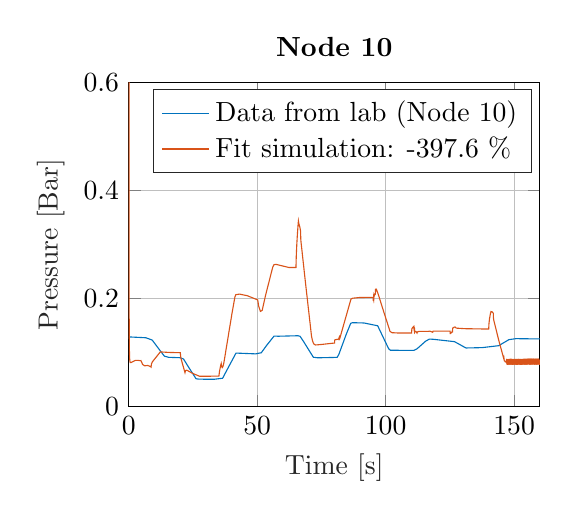
\begin{tikzpicture}

\begin{axis}[%
width=2.0556in,
height=1.62135in,
at={(0.766in,0.486in)},
scale only axis,
xmin=0,
xmax=160,
xlabel style={font=\color{white!15!black}},
xlabel={Time [s]},
ymin=0,
ymax=0.6,
ylabel style={font=\color{white!15!black}},
ylabel={Pressure [Bar]},
axis background/.style={fill=white},
title style={font=\bfseries},
title={Node 10},
xmajorgrids,
ymajorgrids,
legend style={legend cell align=left, align=left, draw=white!15!black}
]
\addplot [color=mycolor1]
  table[row sep=crcr]{%
0.0500000000000114	0.129247487781043\\
6.69999999999999	0.127654535679369\\
9.15000000000001	0.123324594330398\\
12	0.105223577712621\\
13.9	0.0935256891495726\\
15.6	0.0914368426197427\\
20.05	0.0907278005865066\\
21.35	0.0882431085044004\\
22.95	0.0759344868035043\\
26.2	0.0518505474095718\\
27.4	0.0510257966764414\\
33.3	0.0508674584555138\\
36.55	0.0527535972629494\\
37.65	0.0627550048875776\\
41.75	0.0993059042033337\\
49.4	0.0978652003909986\\
51.6	0.0999201173020481\\
53.6	0.113062189638327\\
56.55	0.130669051808411\\
58.35	0.130504623655924\\
65.9	0.13140680351907\\
66.7	0.130314965786908\\
67.9	0.121802111436949\\
71.85	0.0916430303030324\\
73.55	0.0905886021505466\\
81.1	0.0913689833822104\\
81.75	0.0965454252199436\\
84.75	0.135220840664715\\
86.4	0.1543380058651\\
87.1	0.155563822091892\\
91.6	0.154992238514183\\
96.9	0.149808836754659\\
101.15	0.107477722385141\\
101.8	0.104587614858275\\
110.95	0.104193509286404\\
112.2	0.107182795698918\\
115.6	0.121521104594336\\
117.05	0.12521508308896\\
118.65	0.124785307917904\\
126.8	0.120445796676449\\
131.25	0.108748778103632\\
137.55	0.109400400782022\\
144	0.113024780058652\\
147.95	0.124133685239485\\
150.7	0.126004164222877\\
160	0.125475210166172\\
};
\addlegendentry{Data from lab (Node 10)}

\addplot [color=mycolor2]
  table[row sep=crcr]{%
0.0500000000000114	6.25508391238557\\
0.0999999999999943	0.527827712429939\\
0.150000000000006	0.225306397698262\\
0.199999999999989	0.144598185290704\\
0.25	0.113053169762708\\
0.300000000000011	0.0984595621127937\\
0.400000000000006	0.0864269265481425\\
0.550000000000011	0.0818627858579362\\
0.900000000000006	0.0818632895341409\\
2.65000000000001	0.0858975226077803\\
3.19999999999999	0.0857482283952038\\
3.65000000000001	0.0858842940624527\\
4.19999999999999	0.0854063924610102\\
4.75	0.085480576517881\\
5.19999999999999	0.0807640402943548\\
5.34999999999999	0.0784092301410908\\
6.19999999999999	0.075732352086618\\
7.44999999999999	0.0764350252007659\\
8.65000000000001	0.0737652271603793\\
8.69999999999999	0.0735132056768464\\
8.84999999999999	0.0791254223369435\\
9.19999999999999	0.0830472032755551\\
12.3	0.101476498013227\\
15.55	0.10053775735696\\
20.1	0.0999912911644287\\
20.2	0.0933468561705979\\
20.4	0.088291022604011\\
21.9	0.0631468328124924\\
22.1	0.0669244564625728\\
22.6	0.0676975768119235\\
24.7	0.0621169863557043\\
27.55	0.0564531592286244\\
35.1	0.0565940863274932\\
35.35	0.0658496216431956\\
35.8	0.0764627181108324\\
36	0.0798406467007737\\
36.15	0.0746797468667353\\
36.4	0.072439167612032\\
36.7	0.0745451522797111\\
37.05	0.0817907359519836\\
40.2	0.172906844730505\\
41.35	0.203663000994794\\
41.7	0.207342191754066\\
43.1	0.208445987200292\\
46.15	0.205465029606955\\
50.2	0.197736868868759\\
50.6	0.185638397187944\\
51.25	0.176510754464516\\
51.95	0.178308796307846\\
53.25	0.206054511627144\\
56.05	0.258319852971312\\
56.55	0.262972463921301\\
57.3	0.263481094406757\\
62.45	0.257574172461034\\
65.1	0.257756041464035\\
65.15	0.26884294653297\\
65.25	0.283322146652182\\
65.4	0.299016390964283\\
65.65	0.319267904767514\\
65.95	0.338901533738749\\
66.05	0.343741272631775\\
66.15	0.340863366344195\\
66.3	0.33739848503069\\
66.5	0.334322131803702\\
66.7	0.330314612257155\\
66.9	0.324562257351005\\
66.95	0.311003136952792\\
67.05	0.305235595370675\\
68.8	0.229153160589306\\
71.15	0.130381879341428\\
71.55	0.121666167613824\\
72	0.116256519147271\\
72.7	0.114308440063212\\
74.95	0.115213556625662\\
80.1	0.117916045483923\\
80.15	0.122197519776449\\
80.3	0.123990233438633\\
81.65	0.125026410312302\\
81.9	0.128166097604861\\
81.95	0.124761962687472\\
82.1	0.125664970765939\\
86.5	0.199267841090347\\
87.15	0.200865283275334\\
89.9	0.20216147644399\\
95.1	0.202410224154278\\
95.2	0.195906413978065\\
95.25	0.199955738489081\\
95.3	0.198807689279249\\
95.35	0.202791141219762\\
95.4	0.201231006147026\\
95.45	0.204982550041564\\
95.5	0.203121077136814\\
95.55	0.206693305765526\\
95.6	0.204622357997692\\
95.65	0.208025602774939\\
95.7	0.205776427408921\\
95.75	0.20904480999846\\
95.8	0.206673880396323\\
95.85	0.209809245198016\\
95.9	0.207300452251616\\
95.95	0.210285592329257\\
96	0.20763427639605\\
96.05	0.217080607010473\\
96.25	0.217896809754819\\
96.5	0.216233120028562\\
97.25	0.206085986594303\\
98.85	0.181750593345555\\
101.7	0.139433864850162\\
102.45	0.137048818006576\\
105	0.136441594610972\\
110.1	0.136521497731877\\
110.15	0.14163946734152\\
110.25	0.1450009117859\\
110.65	0.147318186494147\\
111	0.148916195788757\\
111.05	0.143313728513419\\
111.2	0.138937795211945\\
111.3	0.140784109690088\\
111.35	0.138129939901802\\
111.5	0.139526186773395\\
111.75	0.139307291533441\\
111.95	0.138228974863893\\
112.2	0.136365509671236\\
112.35	0.138488733958297\\
113	0.13941871066919\\
116.5	0.139455571373475\\
116.85	0.139696042643919\\
117.2	0.139927470926096\\
118.3	0.13788375546406\\
118.45	0.14003685077364\\
125.1	0.140052834356084\\
125.15	0.135400017644457\\
125.3	0.135772616250961\\
125.8	0.138468668838897\\
126	0.138362816315208\\
126.05	0.14345435753583\\
126.15	0.145960127945216\\
126.95	0.147699854787703\\
127.5	0.145454287793257\\
130.9	0.14444769776668\\
140.1	0.143741121797007\\
140.2	0.153283761892538\\
140.4	0.162360105498493\\
140.8	0.173045350586619\\
140.9	0.173822134666324\\
140.95	0.176280455327856\\
141.2	0.17595147550449\\
141.45	0.175564091817506\\
141.9	0.172920963001275\\
141.95	0.164443440333173\\
142.1	0.159469046517614\\
144.05	0.122366040426328\\
146	0.0884182478242792\\
146.05	0.0897171232657286\\
146.15	0.0860916433510113\\
146.55	0.083039159149024\\
146.9	0.0823953675891289\\
146.95	0.0840041288771545\\
147.05	0.0822658383881674\\
147.1	0.083887680927262\\
147.2	0.0821840523462072\\
147.25	0.0838054240814756\\
147.35	0.0821599765366727\\
147.4	0.0837929519414331\\
147.5	0.0821283083689934\\
147.55	0.0837470214518987\\
147.65	0.0820931646439931\\
147.7	0.0837229841912404\\
147.8	0.0821012063948672\\
147.85	0.0837571315015566\\
147.95	0.0821787048084559\\
148	0.083859483154697\\
148.1	0.0822595161294259\\
148.15	0.0839417193636791\\
148.25	0.0823485488296001\\
148.3	0.0840316502130918\\
148.4	0.082390446776742\\
148.45	0.0840735091589124\\
148.55	0.0824006777878026\\
148.6	0.084054482987284\\
148.7	0.0823772323423952\\
148.75	0.0840299442859305\\
148.85	0.0823661954266868\\
148.9	0.0840386355902467\\
149	0.0823862615084465\\
149.05	0.0840429677810448\\
149.15	0.0823652940189561\\
149.2	0.0840155718403253\\
149.3	0.082337588225073\\
149.35	0.0839708251447462\\
149.45	0.0822688587380185\\
149.5	0.0838980126673619\\
149.6	0.0822177201287673\\
149.65	0.0838443324634852\\
149.75	0.0821917284435187\\
149.8	0.083847835550614\\
149.9	0.0822027530333003\\
149.95	0.0838472021798964\\
150.05	0.0822068468956161\\
150.1	0.0838571882413248\\
150.2	0.0822127060941682\\
150.25	0.0838586591704313\\
150.35	0.0821931858589835\\
150.4	0.0838333922180823\\
150.5	0.082180397285299\\
150.55	0.0838333218841001\\
150.65	0.0822220175063251\\
150.7	0.0838703797522555\\
150.8	0.0822225892367783\\
150.85	0.0838799412520075\\
150.95	0.0822399146956343\\
151	0.0838944774384629\\
151.1	0.0822573042671308\\
151.15	0.0839177409824003\\
151.25	0.0822643231474842\\
151.3	0.0839213242250594\\
151.4	0.0822951252842472\\
151.45	0.083959229209654\\
151.55	0.082307751975577\\
151.6	0.0839713819733277\\
151.7	0.0823127427352404\\
151.75	0.0839562974293813\\
151.85	0.0822692216442249\\
151.9	0.0839032878363071\\
152	0.0822316565672736\\
152.05	0.0838657839103973\\
152.15	0.0822058355198578\\
152.2	0.0838463641080409\\
152.3	0.0821962570958021\\
152.35	0.0838451295840912\\
152.45	0.0822079311493553\\
152.5	0.0838497016540884\\
152.6	0.0822172756475936\\
152.65	0.0838696989910659\\
152.75	0.0822428636688528\\
152.8	0.0838986591664366\\
152.9	0.0822527607182337\\
152.95	0.0838943176695466\\
153.05	0.0822379089973708\\
153.1	0.0839092346495534\\
153.2	0.0822877674674203\\
153.25	0.0839425661842199\\
153.35	0.0823154365278072\\
153.4	0.0839942899192181\\
153.5	0.0823668632503427\\
153.55	0.0840527745019131\\
153.65	0.0824360175512879\\
153.7	0.0841317932902825\\
153.8	0.0825123254976745\\
153.85	0.0842023389922986\\
153.95	0.0825257887660769\\
154	0.0842043855112138\\
154.1	0.0825264669503838\\
154.15	0.0842056304358039\\
154.25	0.0825397473844305\\
154.3	0.0842300294595475\\
154.4	0.0825739759714565\\
154.45	0.0842620965775041\\
154.55	0.0825891715511773\\
154.6	0.084283185823864\\
154.7	0.0826198933411888\\
154.75	0.0843023467041633\\
154.85	0.0826135516079205\\
154.9	0.0843143512259417\\
155	0.082657599809437\\
155.05	0.0843606482171708\\
155.15	0.0826662484483336\\
155.2	0.0843526615123551\\
155.3	0.0826675307237679\\
155.35	0.0843605877171854\\
155.45	0.0826725570815938\\
155.5	0.0843670907525507\\
155.6	0.0826736321057524\\
155.65	0.0843597582502582\\
155.75	0.0826499761172101\\
155.8	0.0843339945625701\\
155.9	0.0826453341717013\\
155.95	0.0843410620148859\\
156.05	0.0826514032600301\\
156.1	0.0843387215803943\\
156.2	0.0826573865700766\\
156.25	0.0843617576502993\\
156.35	0.0826700024130105\\
156.4	0.0843524690982349\\
156.5	0.0826626601320299\\
156.55	0.0843552476247282\\
156.65	0.0826773653236899\\
156.7	0.0843712172865594\\
156.8	0.082685626361922\\
156.85	0.0843832597623191\\
156.95	0.0826825573658994\\
157	0.0843764826926474\\
157.1	0.0826959940460483\\
157.15	0.0843914291868657\\
157.25	0.0826923396366794\\
157.3	0.0843768932614353\\
157.4	0.0826707361908348\\
157.45	0.0843551749371443\\
157.55	0.0826576733559534\\
157.6	0.0843397903741163\\
157.7	0.0826367084765138\\
157.75	0.0843300092793697\\
157.85	0.082630393199338\\
157.9	0.0843061321044729\\
158	0.0826352181728112\\
158.05	0.0843285012419983\\
158.15	0.0826393456371193\\
158.2	0.084331493637535\\
158.3	0.0826448412013576\\
158.35	0.0843329472144774\\
158.45	0.082648885981996\\
158.5	0.0843364896811636\\
158.6	0.0826434543327537\\
158.65	0.0843277579148491\\
158.75	0.0826339441381094\\
158.8	0.0843270534078897\\
158.9	0.0826421348454573\\
158.95	0.0843274386687938\\
159.05	0.0826454431023365\\
159.1	0.0843515860265427\\
159.2	0.082676402763866\\
159.25	0.0843633599578766\\
159.35	0.0826498121352017\\
159.4	0.0843360485107496\\
159.5	0.0826410917680107\\
159.55	0.0843275117115354\\
159.65	0.0826206480024041\\
159.7	0.0842897760736321\\
159.8	0.0825903977724636\\
159.85	0.084274824785183\\
159.95	0.0825905001343017\\
160	0.0842732918809759\\
};
\addlegendentry{Fit simulation: -397.6 \%}

\end{axis}
\end{tikzpicture}%
\caption{Step response of one pump PI system.}
\label{fig:Tikz_PI_PUMP_GAIN}
\end{figure}

\begin{figure}[H]
\centering
% This file was created by matlab2tikz.
%
%The latest updates can be retrieved from
%  http://www.mathworks.com/matlabcentral/fileexchange/22022-matlab2tikz-matlab2tikz
%where you can also make suggestions and rate matlab2tikz.
%
\definecolor{mycolor1}{rgb}{0.00000,0.44700,0.74100}%
\definecolor{mycolor2}{rgb}{0.85000,0.32500,0.09800}%
%
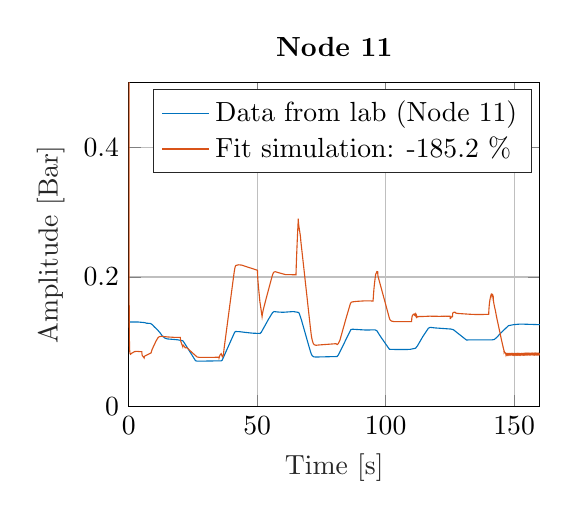
\begin{tikzpicture}

\begin{axis}[%
width=2.0556in,
height=1.62135in,
at={(0.766in,0.486in)},
scale only axis,
xmin=0,
xmax=160,
xlabel style={font=\color{white!15!black}},
xlabel={Time [s]},
ymin=0,
ymax=0.5,
ylabel style={font=\color{white!15!black}},
ylabel={Amplitude [Bar]},
axis background/.style={fill=white},
title style={font=\bfseries},
title={Node 11},
xmajorgrids,
ymajorgrids,
legend style={legend cell align=left, align=left, draw=white!15!black}
]
\addplot [color=mycolor1]
  table[row sep=crcr]{%
0.0500000000000114	0.130694281524939\\
3.69999999999999	0.130651652003905\\
6.19999999999999	0.129741642228737\\
7.05000000000001	0.128711573802548\\
8.34999999999999	0.128618484848488\\
9.09999999999999	0.126835874877798\\
10	0.123143636363636\\
11.35	0.117936744868047\\
12.25	0.113769491691102\\
13	0.10960571847508\\
14	0.105916959921785\\
15.05	0.104589354838708\\
19	0.103262619745834\\
21.1	0.101674887585546\\
21.75	0.0978756402737133\\
26	0.0709816324535666\\
26.75	0.0702499706744959\\
36.05	0.0708328641251228\\
36.4	0.0720186608015752\\
36.8	0.0753716031280476\\
37.7	0.0836208504398712\\
41.25	0.115023147605086\\
41.6	0.116038426197463\\
43.15	0.115747849462366\\
45.35	0.114654271749743\\
47.45	0.11378167155425\\
48.35	0.113434545454538\\
51.1	0.113014340175965\\
51.6	0.114988347996103\\
52.35	0.120243958944286\\
54.45	0.135279130009792\\
56	0.145293587487799\\
56.6	0.146802150537638\\
57.45	0.146352365591412\\
58.5	0.14594521016619\\
60.1	0.145665073313779\\
64.05	0.146789100684259\\
66.15	0.145436265884655\\
66.5	0.142530498533716\\
67.2	0.134222961876844\\
69.35	0.104163929618778\\
70.4	0.0894837145650058\\
71.05	0.0813319061583684\\
71.45	0.0785679472140828\\
72	0.0770237145650015\\
72.8	0.0766670185728344\\
81.1	0.0774613196481084\\
81.6	0.0799025122189789\\
82.65	0.0883153176930591\\
86.45	0.118985953079175\\
87.15	0.119535786901281\\
92.35	0.118275171065505\\
95.1	0.118541388074277\\
95.9	0.118535298142717\\
96.6	0.117141573802542\\
97.25	0.112934301075285\\
98.4	0.105976119257093\\
101.45	0.0886676637341282\\
102.1	0.0884875757575685\\
103.1	0.0883892668621797\\
105.3	0.0881978690127028\\
107.45	0.0883100977517017\\
109.4	0.0883979667644326\\
111.65	0.0902806256109443\\
112.4	0.0940842228739029\\
114.45	0.1081284750733\\
116.6	0.120942561094807\\
117.35	0.122468523949181\\
119.25	0.12153676441838\\
125.4	0.119798523949157\\
126.35	0.118824134897352\\
131.45	0.102863294232662\\
132.35	0.103089491691122\\
138.55	0.103152130987297\\
141.5	0.103189540566973\\
142.3	0.103776783968726\\
143.35	0.107388113392005\\
144.75	0.113558954056685\\
147.8	0.125048914956011\\
149.95	0.1266984164223\\
152.45	0.127498807429134\\
159.15	0.126689716520048\\
160	0.126654046920834\\
};
\addlegendentry{Data from lab (Node 11)}

\addplot [color=mycolor2]
  table[row sep=crcr]{%
0.0500000000000114	2.00785248408209\\
0.0999999999999943	0.495954452939998\\
0.150000000000006	0.214822120013139\\
0.199999999999989	0.139892764121015\\
0.25	0.110624109735994\\
0.300000000000011	0.0968201191140565\\
0.349999999999994	0.089240649874796\\
0.400000000000006	0.0857984666619416\\
0.449999999999989	0.0835589653930242\\
0.550000000000011	0.081613391808304\\
0.699999999999989	0.0808105199786837\\
1.05000000000001	0.0822181549039271\\
2.40000000000001	0.0852589920745572\\
2.84999999999999	0.0852824383850361\\
3.19999999999999	0.0854674512690963\\
3.65000000000001	0.085227686097852\\
4	0.0851989783129454\\
4.34999999999999	0.0849219552197269\\
4.80000000000001	0.0849531081254042\\
5.09999999999999	0.0848985592749614\\
5.15000000000001	0.0818656255914902\\
5.25	0.0792590091787986\\
6	0.0752076836893139\\
6.09999999999999	0.0774368444951676\\
6.34999999999999	0.0784657035187024\\
8.69999999999999	0.0830443683090323\\
9.09999999999999	0.0883737186031794\\
10.6	0.10100666963524\\
11.35	0.106240358555681\\
11.9	0.108100021973314\\
12.7	0.108624857489389\\
15.3	0.107596274445598\\
18.05	0.106924576822308\\
20.1	0.106916696130043\\
20.15	0.103738303295813\\
20.25	0.101147753296146\\
20.5	0.0982381166617188\\
21	0.0929039508237111\\
21.05	0.094598240930253\\
21.2	0.0950400760627303\\
21.55	0.0933922150539388\\
22	0.0908373487058043\\
22.3	0.0915426700041451\\
22.85	0.0904453332024673\\
24.55	0.0839875357556537\\
26.65	0.0766632873681203\\
27.8	0.0760494148437658\\
35.1	0.076303425806401\\
35.15	0.0751981660429806\\
35.35	0.077753076121553\\
35.65	0.0805668097838463\\
36	0.0818564902548928\\
36.45	0.0770588185064298\\
36.65	0.0780859581606705\\
36.9	0.0810628828230051\\
37	0.0856512467164805\\
37.25	0.0936725446374282\\
41	0.206235546631973\\
41.3	0.213595391139876\\
41.5	0.216663574249566\\
41.7	0.217863760228511\\
42.75	0.218896835578448\\
43.9	0.218466659127301\\
49.05	0.211822861043146\\
50.1	0.210492249806521\\
50.15	0.204443240178932\\
50.25	0.196904143285394\\
50.45	0.186734398310932\\
51.05	0.162031413145229\\
51.4	0.152815184447377\\
51.9	0.139065143099486\\
52.05	0.143490992555087\\
52.35	0.149202585231336\\
53.35	0.164783340210704\\
55.85	0.201857805295475\\
56.2	0.205817797670591\\
56.55	0.207768064526761\\
57.05	0.208254159096924\\
58.2	0.20683785173739\\
61	0.203814499130573\\
64.85	0.20352569066219\\
65.1	0.203546869064439\\
65.2	0.216505323575092\\
65.35	0.233088089602433\\
65.55	0.252348180291307\\
65.8	0.274242879091787\\
66	0.289946264467261\\
66.05	0.285314882487086\\
66.15	0.280800108464859\\
66.3	0.276487073207818\\
66.75	0.264936661974673\\
66.9	0.260109303009102\\
66.95	0.256865933847763\\
67.1	0.251317104061258\\
67.65	0.23183116503526\\
70.65	0.123787524883653\\
71.05	0.110597466904323\\
71.25	0.105787148074796\\
71.55	0.10081509009558\\
71.85	0.0974386981781947\\
72.2	0.0956253600754735\\
72.85	0.0947865458151966\\
74.45	0.0953965018816518\\
80.65	0.0972324937155236\\
81.15	0.0959379135056224\\
81.6	0.097543168382316\\
82.2	0.102614908997538\\
84.55	0.135844321602633\\
86.25	0.158793927092148\\
86.55	0.160893224529246\\
87	0.161694308960932\\
88.6	0.162486260221129\\
92.05	0.163338337501045\\
95.1	0.163083593939774\\
95.3	0.174864465627849\\
95.45	0.182149406640775\\
95.7	0.191747320860401\\
96.1	0.204059551876384\\
96.6	0.208497521669983\\
96.9	0.208390058457951\\
96.95	0.203594255422871\\
97.05	0.200749833362408\\
99.05	0.17171783656886\\
101.5	0.135761793645742\\
101.8	0.133518822899077\\
102.3	0.132057196053893\\
103.3	0.131285814442492\\
109.1	0.131316207076594\\
110.1	0.131336463405205\\
110.15	0.135419357058822\\
110.25	0.138699315564082\\
110.45	0.14083370482328\\
110.85	0.142814491498484\\
111.1	0.142926725097368\\
111.15	0.142212257151755\\
111.25	0.142553701719606\\
111.3	0.141878338166009\\
111.4	0.142342164572057\\
111.45	0.141628303648332\\
111.5	0.142015948752999\\
111.55	0.141456112943644\\
111.6	0.142237085785609\\
111.65	0.141449102840795\\
111.8	0.141662496065948\\
111.85	0.140928014210346\\
111.9	0.141287757054243\\
111.95	0.137635178807102\\
112.05	0.137442312735374\\
112.5	0.13935269639785\\
112.65	0.138756631886622\\
113.3	0.139397573476941\\
113.45	0.139107623982369\\
114.15	0.139134938219769\\
117.5	0.139737987253881\\
117.75	0.139559996469984\\
118.4	0.13960357847057\\
118.65	0.139563669302674\\
119.1	0.139634548526629\\
119.35	0.139494182550976\\
120.1	0.139562084402144\\
120.35	0.139359871749065\\
120.7	0.139295704625482\\
121.85	0.139545720065314\\
122.1	0.139434064211258\\
123.15	0.139659676145925\\
123.55	0.139581315031961\\
123.7	0.139653630916996\\
123.85	0.139489356601928\\
124.1	0.139503012599874\\
124.4	0.139593115931461\\
124.6	0.13943068600625\\
125.1	0.139593109242128\\
125.15	0.136068215062295\\
125.25	0.136199967781408\\
125.55	0.138477899574156\\
125.9	0.139052554288725\\
126	0.138890936099557\\
126.05	0.14283070072716\\
126.15	0.144789037052249\\
126.55	0.145661545621692\\
127	0.145850108881604\\
127.3	0.144421136992321\\
128.05	0.143873830821292\\
132.85	0.142604646193149\\
135.35	0.142201099821335\\
140.1	0.142427021597172\\
140.15	0.147512657037055\\
140.25	0.153781800518857\\
140.4	0.15992452050827\\
140.6	0.165446826546372\\
140.85	0.170343025421772\\
141	0.17204614439413\\
141.1	0.173578565853063\\
141.35	0.173595115835724\\
141.4	0.171687535426202\\
141.45	0.173487815146586\\
141.6	0.172982874192144\\
141.9	0.169534031447739\\
141.95	0.163664337550927\\
142.05	0.160540639562271\\
142.25	0.156495514471857\\
142.5	0.15159738926809\\
142.7	0.148512407989983\\
142.9	0.144117443025948\\
143.2	0.137761116915044\\
144.35	0.116640519328399\\
144.65	0.111257193448211\\
144.9	0.106079934800817\\
145.65	0.0931337369363519\\
145.7	0.0916901560873669\\
145.8	0.0907051451764289\\
146	0.0872852871761438\\
146.05	0.0854227703960078\\
146.1	0.0861682912130277\\
146.5	0.0824671436496942\\
146.75	0.081570225823242\\
146.8	0.0805675385979612\\
146.85	0.0816024694625241\\
147.1	0.0802201851909388\\
147.15	0.0813570984040268\\
147.4	0.0801391909618019\\
147.45	0.0812892223949859\\
147.7	0.0800823668236319\\
147.75	0.08124061006734\\
148	0.0801995946976319\\
148.05	0.0813885100350831\\
148.3	0.0803425390934649\\
148.35	0.0815279774160729\\
148.6	0.0803632609393787\\
148.65	0.081531852590615\\
148.9	0.0803521670203224\\
148.95	0.081534819019339\\
149.2	0.0803303516507867\\
149.25	0.0814964140994334\\
149.5	0.0802298615365373\\
149.55	0.0813795329224547\\
149.8	0.080188737091504\\
149.85	0.0813547553835861\\
150.1	0.0801950865443644\\
150.15	0.0813593834229209\\
150.4	0.080175310201156\\
150.45	0.0813326056395454\\
150.7	0.0802038358965547\\
150.75	0.081366991541671\\
151	0.0802284042288477\\
151.05	0.0814004437438598\\
151.3	0.080253772564248\\
151.35	0.0814322030000199\\
151.6	0.0802925336009537\\
151.65	0.0814649620240289\\
151.9	0.0802354380577697\\
151.95	0.081390731127243\\
152.2	0.080186236957843\\
152.25	0.0813464040962799\\
152.5	0.0801894331940503\\
152.55	0.0813586189009072\\
152.8	0.0802320463354818\\
152.85	0.0814026897717781\\
153.1	0.0802454759246132\\
153.15	0.0814309412143643\\
153.4	0.0803139720020738\\
153.45	0.0815011928910963\\
153.7	0.0804323440281962\\
153.75	0.0816401066469439\\
154	0.0804909902042823\\
154.05	0.0816752757070276\\
154.3	0.0805140056257869\\
154.35	0.0817124188596381\\
154.6	0.0805589149647972\\
154.65	0.0817603557377424\\
154.9	0.0805868052923699\\
154.95	0.0817926755691758\\
155.2	0.0806169997302391\\
155.25	0.0818111300487203\\
155.5	0.0806270060579948\\
155.55	0.0818214220942082\\
155.8	0.0806009105674548\\
155.85	0.0817911847398136\\
156.1	0.0806049732195504\\
156.15	0.0817983344981883\\
156.4	0.0806152848072088\\
156.45	0.0818077944267657\\
156.7	0.0806314530076122\\
156.75	0.0818283667529727\\
157	0.0806389479105292\\
157.05	0.0818395700776477\\
157.3	0.080635978179231\\
157.35	0.0818237925463166\\
157.6	0.0806026824860453\\
157.65	0.0817865618811595\\
157.9	0.0805784158754079\\
157.95	0.0817721967035254\\
158.2	0.0805989337164306\\
158.25	0.0817926474936712\\
158.5	0.0806014097032346\\
158.55	0.0817920580415432\\
158.8	0.0805950016283532\\
158.85	0.0817890766887501\\
159.1	0.0806156692213449\\
159.15	0.0818183250543711\\
159.4	0.0806018856726496\\
159.45	0.0817899643030273\\
159.7	0.0805625651047706\\
159.75	0.0817422094887377\\
160	0.080549161511442\\
};
\addlegendentry{Fit simulation: -185.2 \%}

\end{axis}
\end{tikzpicture}%
\caption{Step response of one pump PI system.}
\label{fig:Tikz_PI_PUMP_GAIN}
\end{figure}

\begin{figure}[H]
\centering
% This file was created by matlab2tikz.
%
%The latest updates can be retrieved from
%  http://www.mathworks.com/matlabcentral/fileexchange/22022-matlab2tikz-matlab2tikz
%where you can also make suggestions and rate matlab2tikz.
%
\definecolor{mycolor1}{rgb}{0.00000,0.44700,0.74100}%
\definecolor{mycolor2}{rgb}{0.85000,0.32500,0.09800}%
%
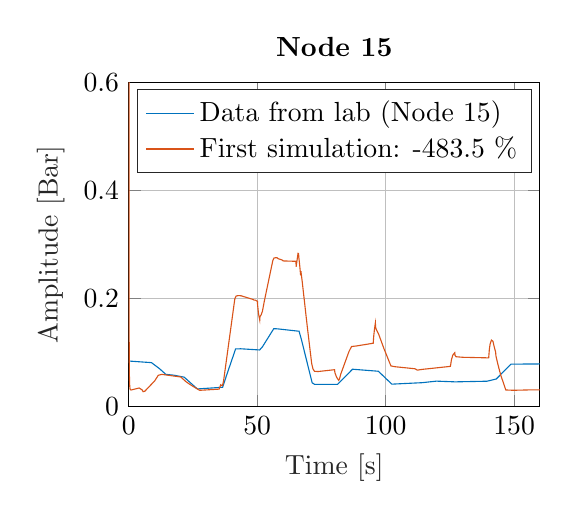
\begin{tikzpicture}

\begin{axis}[%
width=2.0556in,
height=1.62135in,
at={(0.766in,0.486in)},
scale only axis,
xmin=0,
xmax=160,
xlabel style={font=\color{white!15!black}},
xlabel={Time [s]},
ymin=0,
ymax=0.6,
ylabel style={font=\color{white!15!black}},
ylabel={Amplitude [Bar]},
axis background/.style={fill=white},
title style={font=\bfseries},
title={Node 15},
xmajorgrids,
ymajorgrids,
legend style={legend cell align=left, align=left, draw=white!15!black}
]
\addplot [color=mycolor1]
  table[row sep=crcr]{%
0.0500000000000114	0.0845804496578637\\
8.84999999999999	0.0816346627565849\\
11.95	0.0706084066471249\\
14.45	0.0599231867057597\\
17.5	0.0584589931573873\\
21.6	0.054695415444769\\
26.7	0.0329552297165208\\
36.55	0.0360610948191606\\
38	0.0570348191593268\\
41.6	0.106960078201382\\
43.55	0.107266314760523\\
50.95	0.105078289345073\\
52.05	0.110984652981415\\
56.45	0.144457526881723\\
57.9	0.144153030303016\\
66.3	0.139736959921805\\
67.2	0.124550410557191\\
71.4	0.0442581427174957\\
72.35	0.0414767839687329\\
81.25	0.041502883675463\\
82.6	0.0476215249266829\\
87.1	0.0694365298142827\\
97.15	0.0657007917888563\\
102.4	0.0418195601173181\\
114.2	0.0445356695992132\\
119.75	0.0473901075268941\\
127.05	0.0460729423265036\\
139.45	0.0472448191593458\\
143.05	0.0513711827956911\\
148.75	0.0788533040078221\\
160	0.0792230498533684\\
};
\addlegendentry{Data from lab (Node 15)}

\addplot [color=mycolor2]
  table[row sep=crcr]{%
0.0500000000000114	9.65583948912268\\
0.0999999999999943	0.497739745062006\\
0.150000000000006	0.184910944604326\\
0.199999999999989	0.100894856102343\\
0.25	0.0675119874345\\
0.300000000000011	0.0514005048865442\\
0.400000000000006	0.0378149451047989\\
0.550000000000011	0.0320158005750955\\
0.900000000000006	0.0309547850295075\\
4.05000000000001	0.0347081168541195\\
5.19999999999999	0.03131369765768\\
5.59999999999999	0.0279126597350228\\
6.25	0.0286625960735023\\
10.1	0.0478055629008054\\
11.5	0.058166076660882\\
12.85	0.05992449253921\\
20.25	0.0550638130074503\\
22.3	0.0463594168655845\\
23.95	0.0409047684521795\\
27.6	0.0304011742361183\\
35.2	0.0325981451582322\\
35.8	0.0406308455723376\\
36.15	0.0394962664888681\\
36.5	0.039275679861106\\
36.9	0.0474681490297257\\
37.35	0.0626687703682478\\
41.3	0.199861244146263\\
41.85	0.204988717217162\\
42.6	0.205656638605063\\
42.75	0.205678942620324\\
43.8	0.20535019597213\\
43.9	0.205063124053396\\
48.45	0.198433238458904\\
48.8	0.197269671815775\\
49.15	0.197387898772149\\
49.45	0.196969647185171\\
49.8	0.195839751827464\\
50.1	0.195414831410091\\
50.15	0.188573282989211\\
50.55	0.171215491381361\\
51	0.160297695441926\\
51.1	0.167062320403744\\
51.55	0.169979939941442\\
52.05	0.176844257413478\\
52.75	0.19479048041336\\
56.1	0.270942515744309\\
56.6	0.275498777446188\\
57.7	0.275786704326492\\
58.2	0.273960718716921\\
59.8	0.271306079137105\\
60.1	0.269820759522446\\
65.1	0.269118694005982\\
65.15	0.258851863286338\\
65.9	0.283829563681763\\
66.1	0.28322243802549\\
66.25	0.274701059929271\\
66.6	0.259140844037319\\
66.9	0.243212988592859\\
66.95	0.249920766714098\\
67.05	0.249915050810188\\
67.55	0.230441869609649\\
69.45	0.150068597566985\\
71.2	0.080299700155706\\
71.7	0.0701767986901984\\
72.3	0.0655052323882614\\
73.75	0.065204322876923\\
80.1	0.0685557177792759\\
80.25	0.0629159354867568\\
80.9	0.0546978906295408\\
81.7	0.048948265954607\\
82	0.0510488175005719\\
82.55	0.0607008013298582\\
85.7	0.101935059827525\\
86.7	0.111400935427241\\
88.65	0.112510290171997\\
95.15	0.117516444292789\\
95.35	0.130364842457141\\
95.65	0.143816899160157\\
96	0.154994425756655\\
96.1	0.147287889526979\\
96.35	0.143120060619935\\
97.3	0.133974056277168\\
99.35	0.107364414405254\\
102.05	0.0755245683119483\\
103.7	0.0740518597806101\\
111.4	0.0702982464933655\\
112.35	0.0677805886062117\\
114.15	0.0691097282988835\\
125.2	0.0747240202889827\\
125.6	0.0869039396214077\\
126.15	0.0958307330879791\\
126.9	0.0999827572929632\\
127	0.0951177455772552\\
127.4	0.0925976309382008\\
129.95	0.0915247565368986\\
140.1	0.0904543256477268\\
140.35	0.10615325174021\\
140.65	0.115931595904556\\
141.15	0.123377491709306\\
141.75	0.121316985669637\\
142.15	0.11277863909001\\
142.8	0.100918120047737\\
142.9	0.0944519204483072\\
143.6	0.0799804818790335\\
143.95	0.0738470948553243\\
144.05	0.0712208267260053\\
144.25	0.0684041213786486\\
144.35	0.0658326534488367\\
144.55	0.0631399719402737\\
144.65	0.060563784654903\\
146.75	0.0310799494015725\\
149.6	0.0304512253810856\\
157.2	0.0313209718199801\\
160	0.0312800983863042\\
};
\addlegendentry{First simulation: -483.5 \%}

\end{axis}
\end{tikzpicture}%
\caption{Step response of one pump PI system.}
\label{fig:Tikz_PI_PUMP_GAIN}
\end{figure}

\begin{figure}[H]
\centering
% This file was created by matlab2tikz.
%
%The latest updates can be retrieved from
%  http://www.mathworks.com/matlabcentral/fileexchange/22022-matlab2tikz-matlab2tikz
%where you can also make suggestions and rate matlab2tikz.
%
\definecolor{mycolor1}{rgb}{0.00000,0.44700,0.74100}%
\definecolor{mycolor2}{rgb}{0.85000,0.32500,0.09800}%
%
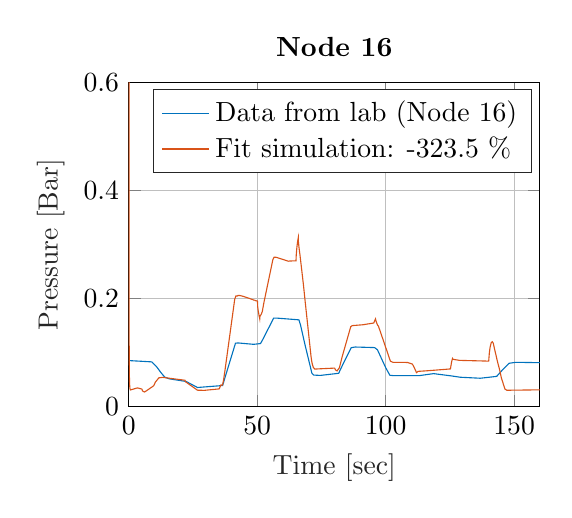
\begin{tikzpicture}

\begin{axis}[%
width=2.0556in,
height=1.62135in,
at={(0.766in,0.486in)},
scale only axis,
xmin=0,
xmax=160,
xlabel style={font=\color{white!15!black}},
xlabel={Time [sec]},
ymin=0,
ymax=0.6,
ylabel style={font=\color{white!15!black}},
ylabel={Pressure [Bar]},
axis background/.style={fill=white},
title style={font=\bfseries},
title={Node 16},
xmajorgrids,
ymajorgrids,
legend style={legend cell align=left, align=left, draw=white!15!black}
]
\addplot [color=mycolor1]
  table[row sep=crcr]{%
0.0500000000000114	0.0854469599217964\\
9	0.0830370869990134\\
10.85	0.0740700977517008\\
12.5	0.0634353372433907\\
14	0.0549346627566081\\
15.75	0.0516765493646005\\
22.35	0.0467776344086133\\
26.75	0.035629579667642\\
36.55	0.0392696187683157\\
37.55	0.0552174095796545\\
41.55	0.117548729227764\\
42.55	0.118078553274671\\
48.6	0.11549729227761\\
51.3	0.116937126099714\\
52.4	0.126468739002945\\
56.4	0.163987067448687\\
57.5	0.164062756598241\\
60.95	0.162792570869982\\
66.25	0.16080986314762\\
66.9	0.150622277614872\\
68.6	0.114903088954065\\
71.3	0.0618884946236449\\
72	0.0585912316715564\\
74.6	0.0579822385141711\\
81.7	0.0618867546432114\\
83.55	0.0803383773215955\\
86.6	0.109338631476049\\
88.15	0.11052268817204\\
95.7	0.109487399804493\\
96.8	0.105386265884647\\
100.05	0.0719316617790753\\
101.65	0.0582371456500539\\
103	0.0576046627566029\\
113.1	0.0576046627566029\\
118.65	0.0612942913001007\\
125.6	0.0570435190615797\\
129.05	0.0546066764418356\\
136.8	0.0527562072336423\\
143.2	0.0561735288367515\\
145.6	0.0688962658846606\\
148.05	0.0804288563049909\\
150.6	0.0822210361681357\\
160	0.08157202346041\\
};
\addlegendentry{Data from lab (Node 16)}

\addplot [color=mycolor2]
  table[row sep=crcr]{%
0.0500000000000114	7.81748507041465\\
0.0999999999999943	0.465512167911328\\
0.150000000000006	0.173770260157823\\
0.199999999999989	0.0955721356373829\\
0.25	0.0645843143310287\\
0.300000000000011	0.0496835521292951\\
0.349999999999994	0.0417245195478415\\
0.449999999999989	0.0344778646394559\\
0.650000000000006	0.0310002202077158\\
1.25	0.0319119134991013\\
3.40000000000001	0.0349006951418289\\
5.15000000000001	0.0326740938036494\\
5.34999999999999	0.0294165771533983\\
6.09999999999999	0.0271978998252109\\
6.84999999999999	0.0293221199800371\\
9.75	0.0389614788549295\\
10.4	0.0457648055505615\\
11.75	0.0535423492885627\\
13.3	0.0543203295787293\\
21.9	0.0490283622173138\\
22.05	0.0464255770514796\\
26.75	0.0306389341515967\\
29.4	0.030331260571586\\
35.25	0.0330500089906138\\
35.8	0.0401053281937891\\
36.15	0.0402962331764058\\
36.5	0.0403315446254169\\
36.85	0.0475666434650464\\
37.45	0.0667624636546407\\
41.25	0.198761717535461\\
41.7	0.204890675883178\\
42.3	0.204982155107274\\
42.5	0.205840200224344\\
43.35	0.205793077516432\\
44.4	0.204429285497184\\
44.55	0.204288296106029\\
47.2	0.20005598663812\\
47.65	0.199089745962624\\
48.1	0.198649226337636\\
48.55	0.1975432879604\\
49	0.197181478857914\\
49.45	0.196236322493718\\
49.9	0.19589740052777\\
50.1	0.195616968647386\\
50.2	0.185019992324982\\
50.4	0.177669742856125\\
50.7	0.169536132597756\\
51	0.162467159617734\\
51.1	0.167961298719149\\
51.55	0.170779840308569\\
52	0.176436655462823\\
52.6	0.192414876626856\\
56.1	0.272185659261112\\
56.6	0.276797475367005\\
57.45	0.276502030362565\\
62.1	0.269321622212061\\
62.75	0.269719366293458\\
65.1	0.269960377618389\\
65.2	0.280556138050997\\
65.45	0.295066485233036\\
65.75	0.306359062171452\\
66	0.312918448390292\\
66.05	0.304936753688196\\
66.3	0.293672257826842\\
66.7	0.279045972314805\\
68	0.225565158637949\\
68.65	0.195741508493995\\
71	0.0912209107730746\\
71.35	0.0808832201269922\\
71.85	0.0725564327337338\\
72.45	0.0696686458908573\\
74.1	0.0701523371992039\\
80.15	0.0715287667857751\\
80.5	0.068004733381855\\
81.1	0.0663771199500047\\
82	0.0721845637498859\\
83.1	0.0930893991442474\\
86.4	0.147990372379951\\
87	0.150148125050407\\
91.1	0.151700845405713\\
95.35	0.154926460835867\\
96.05	0.162631684645021\\
96.3	0.157776136348303\\
96.65	0.153387060800384\\
96.95	0.150331070370555\\
97.15	0.149605927818925\\
98.25	0.134483879221648\\
101.85	0.0842559727217065\\
102.85	0.0822239600503281\\
108.55	0.0819430542063344\\
110.4	0.0789906153822244\\
111.15	0.0721538482435733\\
112	0.0631748115218329\\
112.65	0.065489998480416\\
116.3	0.0666174458243063\\
125.2	0.0699624094023932\\
125.65	0.082783249631035\\
126	0.0893952408953851\\
126.2	0.0878773069876786\\
128.7	0.0858256327078379\\
140.1	0.0844237223077187\\
140.35	0.0996088814561915\\
140.65	0.110319284099376\\
141.1	0.118854788573913\\
141.5	0.120295388863155\\
141.9	0.117348853531666\\
142.35	0.107149456255598\\
142.9	0.0962827094722627\\
143.45	0.0847355462387611\\
144.35	0.0683420372826617\\
145.05	0.0529834227285448\\
146.45	0.0324518585455564\\
147.2	0.0305368799956796\\
160	0.0312906253486176\\
};
\addlegendentry{Fit simulation: -323.5 \%}

\end{axis}
\end{tikzpicture}%
\caption{Step response of one pump PI system.}
\label{fig:Tikz_PI_PUMP_GAIN}
\end{figure}